% -----------------------------------------------------------------------------
%                                     HEADER                                    
% -----------------------------------------------------------------------------
\documentclass[a4paper, 10pt]{article}
\usepackage{jheppub}
\usepackage[T1]{fontenc}
\usepackage{colortbl,xcolor,float}
\definecolor{orange}{rgb}{1,0.5,0}
% -----------------------------------------------------------------------------
%                                   COVER PAGE                                  
% -----------------------------------------------------------------------------
\title{{\includegraphics[scale=.4]{logo.eps}}\ The LaTeX report}

\author{Generated by elijahsheridan on 21 March 2020, 16:38:57}

\abstract{
  This report has been generated automatically
  by {\sc MadAnalysis} 5.\\$~$\\ 
  Please cite:\\ 
  \begin{quote}
    \textbf{E.~Conte, B.~Fuks and G.~Serret},\\ 
    \textit{MadAnalysis 5, A User-Friendly
    Framework for Collider Phenomenology},\\ 
    Comput. Phys. Commun. {\bf 184} (2013) 222-256,\\
    arXiv:1206.1599 [hep-ph].\\ 
  \end{quote}
  To contact us:\\ 
  \begin{quote}
    \textbf{http://madanalysis.irmp.ucl.ac.be}\\
    \textbf{ma5team@iphc.cnrs.fr}\\
  \end{quote}
}

% -----------------------------------------------------------------------------
%                                 BEGIN DOCUMENT                                
% -----------------------------------------------------------------------------
\begin{document}
\maketitle
\flushbottom

% -----------------------------------------------------------------------------
%                                 SECTION Setup                                 
% -----------------------------------------------------------------------------
\newpage
\section{ Setup}

\subsection{ Command history}

\texttt{ma5>\# set directory where running "./\-bin/\-ma5"; set lumi; define the signal significance\\
}
\texttt{ }\texttt{ }\texttt{ma5>set main.currentdir = /\-Users/\-elijahsheridan/\-MG5\_aMC\_v2\_6\_5/\-axion\_data \# need to change this directory path --> exit and type "pwd" to get the path\\
}
\texttt{ }\texttt{ }\texttt{ma5>set main.lumi = 40.0\\
}
\texttt{ }\texttt{ }\texttt{ma5>set main.SBratio = 'S/\-sqrt(S+B)'\\
}
\texttt{ }\texttt{ }\texttt{ma5>\# import samples --> change the path to the LHE file\\
}
\texttt{ }\texttt{ }\texttt{ma5>import /\-Users/\-elijahsheridan/\-MG5\_aMC\_v2\_6\_5/\-axion\_data/\-axion\_signal/\-axion\_signal\_gurrola\_cuts\_1MeV.lhe.gz as signal\\
}
\texttt{ }\texttt{ }\texttt{ma5>import /\-Users/\-elijahsheridan/\-MG5\_aMC\_v2\_6\_5/\-axion\_data/\-vbf\_diphoton\_background\_data/\-merged\_lhe/\-vbf\_diphoton\_background\_ht\_0\_100\_merged.lhe.gz as bg\_vbf\_0\_100\\
}
\texttt{ }\texttt{ }\texttt{ma5>import /\-Users/\-elijahsheridan/\-MG5\_aMC\_v2\_6\_5/\-axion\_data/\-vbf\_diphoton\_background\_data/\-merged\_lhe/\-vbf\_diphoton\_background\_ht\_100\_200\_merged.lhe.gz as bg\_vbf\_100\_200\\
}
\texttt{ }\texttt{ }\texttt{ma5>import /\-Users/\-elijahsheridan/\-MG5\_aMC\_v2\_6\_5/\-axion\_data/\-vbf\_diphoton\_background\_data/\-merged\_lhe/\-vbf\_diphoton\_background\_ht\_200\_400\_merged.lhe.gz as bg\_vbf\_200\_400\\
}
\texttt{ }\texttt{ }\texttt{ma5>import /\-Users/\-elijahsheridan/\-MG5\_aMC\_v2\_6\_5/\-axion\_data/\-vbf\_diphoton\_background\_data/\-merged\_lhe/\-vbf\_diphoton\_background\_ht\_400\_600\_merged.lhe.gz as bg\_vbf\_400\_600\\
}
\texttt{ }\texttt{ }\texttt{ma5>import /\-Users/\-elijahsheridan/\-MG5\_aMC\_v2\_6\_5/\-axion\_data/\-vbf\_diphoton\_background\_data/\-merged\_lhe/\-vbf\_diphoton\_background\_ht\_600\_800\_merged.lhe.gz as bg\_vbf\_600\_800\\
}
\texttt{ }\texttt{ }\texttt{ma5>import /\-Users/\-elijahsheridan/\-MG5\_aMC\_v2\_6\_5/\-axion\_data/\-vbf\_diphoton\_background\_data/\-merged\_lhe/\-vbf\_diphoton\_background\_ht\_800\_1200\_merged.lhe.gz as bg\_vbf\_800\_1200\\
}
\texttt{ }\texttt{ }\texttt{ma5>import /\-Users/\-elijahsheridan/\-MG5\_aMC\_v2\_6\_5/\-axion\_data/\-vbf\_diphoton\_background\_data/\-merged\_lhe/\-vbf\_diphoton\_background\_ht\_1200\_1600\_merged.lhe.gz as bg\_vbf\_1200\_1600\\
}
\texttt{ }\texttt{ }\texttt{ma5>import /\-Users/\-elijahsheridan/\-MG5\_aMC\_v2\_6\_5/\-axion\_data/\-vbf\_diphoton\_background\_data/\-merged\_lhe/\-vbf\_diphoton\_background\_ht\_1600\_inf\_merged.lhe.gz as bg\_vbf\_1600\_inf\\
}
\texttt{ }\texttt{ }\texttt{ma5>import /\-Users/\-elijahsheridan/\-MG5\_aMC\_v2\_6\_5/\-axion\_data/\-diphoton\_double\_isr\_background\_data/\-merged\_lhe/\-diphoton\_double\_isr\_background\_ht\_0\_100\_merged.lhe.gz as bg\_dip\_0\_100\\
}
\texttt{ }\texttt{ }\texttt{ma5>import /\-Users/\-elijahsheridan/\-MG5\_aMC\_v2\_6\_5/\-axion\_data/\-diphoton\_double\_isr\_background\_data/\-merged\_lhe/\-diphoton\_double\_isr\_background\_ht\_100\_200\_merged.lhe.gz as bg\_dip\_100\_200\\
}
\texttt{ }\texttt{ }\texttt{ma5>import /\-Users/\-elijahsheridan/\-MG5\_aMC\_v2\_6\_5/\-axion\_data/\-diphoton\_double\_isr\_background\_data/\-merged\_lhe/\-diphoton\_double\_isr\_background\_ht\_200\_400\_merged.lhe.gz as bg\_dip\_200\_400\\
}
\texttt{ }\texttt{ }\texttt{ma5>import /\-Users/\-elijahsheridan/\-MG5\_aMC\_v2\_6\_5/\-axion\_data/\-diphoton\_double\_isr\_background\_data/\-merged\_lhe/\-diphoton\_double\_isr\_background\_ht\_400\_600\_merged.lhe.gz as bg\_dip\_400\_600\\
}
\texttt{ }\texttt{ }\texttt{ma5>import /\-Users/\-elijahsheridan/\-MG5\_aMC\_v2\_6\_5/\-axion\_data/\-diphoton\_double\_isr\_background\_data/\-merged\_lhe/\-diphoton\_double\_isr\_background\_ht\_600\_800\_merged.lhe.gz as bg\_dip\_600\_800\\
}
\texttt{ }\texttt{ }\texttt{ma5>import /\-Users/\-elijahsheridan/\-MG5\_aMC\_v2\_6\_5/\-axion\_data/\-diphoton\_double\_isr\_background\_data/\-merged\_lhe/\-diphoton\_double\_isr\_background\_ht\_800\_1200\_merged.lhe.gz as bg\_dip\_800\_1200\\
}
\texttt{ }\texttt{ }\texttt{ma5>import /\-Users/\-elijahsheridan/\-MG5\_aMC\_v2\_6\_5/\-axion\_data/\-diphoton\_double\_isr\_background\_data/\-merged\_lhe/\-diphoton\_double\_isr\_background\_ht\_1200\_1600\_merged.lhe.gz as bg\_dip\_1200\_1600\\
}
\texttt{ }\texttt{ }\texttt{ma5>import /\-Users/\-elijahsheridan/\-MG5\_aMC\_v2\_6\_5/\-axion\_data/\-diphoton\_double\_isr\_background\_data/\-merged\_lhe/\-diphoton\_double\_isr\_background\_ht\_1600\_inf\_merged.lhe.gz as bg\_dip\_1600\_inf\\
}
\texttt{ }\texttt{ }\texttt{ma5>\# define bg and signal samples\\
}
\texttt{ }\texttt{ }\texttt{ma5>set signal.type = signal\\
}
\texttt{ }\texttt{ }\texttt{ma5>set bg\_vbf\_0\_100.type = background\\
}
\texttt{ }\texttt{ }\texttt{ma5>set bg\_vbf\_100\_200.type = background\\
}
\texttt{ }\texttt{ }\texttt{ma5>set bg\_vbf\_200\_400.type  = background\\
}
\texttt{ }\texttt{ }\texttt{ma5>set bg\_vbf\_400\_600.type  = background\\
}
\texttt{ }\texttt{ }\texttt{ma5>set bg\_vbf\_600\_800.type  = background\\
}
\texttt{ }\texttt{ }\texttt{ma5>set bg\_vbf\_800\_1200.type  = background\\
}
\texttt{ }\texttt{ }\texttt{ma5>set bg\_vbf\_1200\_1600.type  = background\\
}
\texttt{ }\texttt{ }\texttt{ma5>set bg\_vbf\_1600\_inf.type = background\\
}
\texttt{ }\texttt{ }\texttt{ma5>set bg\_dip\_0\_100.type = background\\
}
\texttt{ }\texttt{ }\texttt{ma5>set bg\_dip\_100\_200.type = background\\
}
\texttt{ }\texttt{ }\texttt{ma5>set bg\_dip\_200\_400.type = background\\
}
\texttt{ }\texttt{ }\texttt{ma5>set bg\_dip\_400\_600.type = background\\
}
\texttt{ }\texttt{ }\texttt{ma5>set bg\_dip\_600\_800.type = background\\
}
\texttt{ }\texttt{ }\texttt{ma5>set bg\_dip\_800\_1200.type = background\\
}
\texttt{ }\texttt{ }\texttt{ma5>set bg\_dip\_1200\_1600.type = background\\
}
\texttt{ }\texttt{ }\texttt{ma5>set bg\_dip\_1600\_inf.type = background\\
}
\texttt{ }\texttt{ }\texttt{ma5>\# define weights for the samples\\
}
\texttt{ }\texttt{ }\texttt{ma5>\#set sample\_1.weight = 1\\
}
\texttt{ }\texttt{ }\texttt{ma5>\#set sample\_2.weight = 1\\
}
\texttt{ }\texttt{ }\texttt{ma5>\# line styles and colors\\
}
\texttt{ }\texttt{ }\texttt{ma5>set signal.linecolor = red\\
}
\texttt{ }\texttt{ }\texttt{ma5>set signal.linestyle = dashed\\
}
\texttt{ }\texttt{ }\texttt{ma5>set signal.linewidth = 3\\
}
\texttt{ }\texttt{ }\texttt{ma5>set bg\_vbf\_0\_100.linecolor = blue-4\\
}
\texttt{ }\texttt{ }\texttt{ma5>set bg\_vbf\_0\_100.linestyle = dash-dotted\\
}
\texttt{ }\texttt{ }\texttt{ma5>set bg\_vbf\_0\_100.linewidth = 4\\
}
\texttt{ }\texttt{ }\texttt{ma5>set bg\_vbf\_100\_200.linecolor = blue-3\\
}
\texttt{ }\texttt{ }\texttt{ma5>set bg\_vbf\_100\_200.linestyle = dash-dotted\\
}
\texttt{ }\texttt{ }\texttt{ma5>set bg\_vbf\_100\_200.linewidth = 4\\
}
\texttt{ }\texttt{ }\texttt{ma5>set bg\_vbf\_200\_400.linecolor = blue-2\\
}
\texttt{ }\texttt{ }\texttt{ma5>set bg\_vbf\_200\_400.linestyle = dash-dotted\\
}
\texttt{ }\texttt{ }\texttt{ma5>set bg\_vbf\_200\_400.linewidth = 4\\
}
\texttt{ }\texttt{ }\texttt{ma5>set bg\_vbf\_400\_600.linecolor = blue-1\\
}
\texttt{ }\texttt{ }\texttt{ma5>set bg\_vbf\_400\_600.linestyle = dash-dotted\\
}
\texttt{ }\texttt{ }\texttt{ma5>set bg\_vbf\_400\_600.linewidth = 4\\
}
\texttt{ }\texttt{ }\texttt{ma5>set bg\_vbf\_600\_800.linecolor = blue\\
}
\texttt{ }\texttt{ }\texttt{ma5>set bg\_vbf\_600\_800.linestyle = dash-dotted\\
}
\texttt{ }\texttt{ }\texttt{ma5>set bg\_vbf\_600\_800.linewidth = 4\\
}
\texttt{ }\texttt{ }\texttt{ma5>set bg\_vbf\_800\_1200.linecolor = blue+1\\
}
\texttt{ }\texttt{ }\texttt{ma5>set bg\_vbf\_800\_1200.linestyle = dash-dotted\\
}
\texttt{ }\texttt{ }\texttt{ma5>set bg\_vbf\_800\_1200.linewidth = 4\\
}
\texttt{ }\texttt{ }\texttt{ma5>set bg\_vbf\_1200\_1600.linecolor = blue+2\\
}
\texttt{ }\texttt{ }\texttt{ma5>set bg\_vbf\_1200\_1600.linestyle = dash-dotted\\
}
\texttt{ }\texttt{ }\texttt{ma5>set bg\_vbf\_1200\_1600.linewidth = 4\\
}
\texttt{ }\texttt{ }\texttt{ma5>set bg\_vbf\_1600\_inf.linecolor = blue+3\\
}
\texttt{ }\texttt{ }\texttt{ma5>set bg\_vbf\_1600\_inf.linestyle = dash-dotted\\
}
\texttt{ }\texttt{ }\texttt{ma5>set bg\_vbf\_1600\_inf.linewidth = 4\\
}
\texttt{ }\texttt{ }\texttt{ma5>set bg\_dip\_0\_100.linecolor = green-4\\
}
\texttt{ }\texttt{ }\texttt{ma5>set bg\_dip\_0\_100.linestyle = dash-dotted\\
}
\texttt{ }\texttt{ }\texttt{ma5>set bg\_dip\_0\_100.linewidth = 4\\
}
\texttt{ }\texttt{ }\texttt{ma5>set bg\_dip\_100\_200.linecolor = green-3\\
}
\texttt{ }\texttt{ }\texttt{ma5>set bg\_dip\_100\_200.linestyle = dash-dotted\\
}
\texttt{ }\texttt{ }\texttt{ma5>set bg\_dip\_100\_200.linewidth = 4\\
}
\texttt{ }\texttt{ }\texttt{ma5>set bg\_dip\_200\_400.linecolor = green-2\\
}
\texttt{ }\texttt{ }\texttt{ma5>set bg\_dip\_200\_400.linestyle = dash-dotted\\
}
\texttt{ }\texttt{ }\texttt{ma5>set bg\_dip\_200\_400.linewidth = 4\\
}
\texttt{ }\texttt{ }\texttt{ma5>set bg\_dip\_400\_600.linecolor = green-1\\
}
\texttt{ }\texttt{ }\texttt{ma5>set bg\_dip\_400\_600.linestyle = dash-dotted\\
}
\texttt{ }\texttt{ }\texttt{ma5>set bg\_dip\_400\_600.linewidth = 4\\
}
\texttt{ }\texttt{ }\texttt{ma5>set bg\_dip\_600\_800.linecolor = green\\
}
\texttt{ }\texttt{ }\texttt{ma5>set bg\_dip\_600\_800.linestyle = dash-dotted\\
}
\texttt{ }\texttt{ }\texttt{ma5>set bg\_dip\_600\_800.linewidth = 4\\
}
\texttt{ }\texttt{ }\texttt{ma5>set bg\_dip\_800\_1200.linecolor = green+1\\
}
\texttt{ }\texttt{ }\texttt{ma5>set bg\_dip\_800\_1200.linestyle = dash-dotted\\
}
\texttt{ }\texttt{ }\texttt{ma5>set bg\_dip\_800\_1200.linewidth = 4\\
}
\texttt{ }\texttt{ }\texttt{ma5>set bg\_dip\_1200\_1600.linecolor = green+2\\
}
\texttt{ }\texttt{ }\texttt{ma5>set bg\_dip\_1200\_1600.linestyle = dash-dotted\\
}
\texttt{ }\texttt{ }\texttt{ma5>set bg\_dip\_1200\_1600.linewidth = 4\\
}
\texttt{ }\texttt{ }\texttt{ma5>set bg\_dip\_1600\_inf.linecolor = green+3\\
}
\texttt{ }\texttt{ }\texttt{ma5>set bg\_dip\_1600\_inf.linestyle = dash-dotted\\
}
\texttt{ }\texttt{ }\texttt{ma5>set bg\_dip\_1600\_inf.linewidth = 4\\
}
\texttt{ }\texttt{ }\texttt{ma5>\# a jet can be from a light quark or b quark\\
}
\texttt{ }\texttt{ }\texttt{ma5>define jets = j\\
}
\texttt{ }\texttt{ }\texttt{ma5>define e = e+ e-\\
}
\texttt{ }\texttt{ }\texttt{ma5>define mu = mu+ mu-\\
}
\texttt{ }\texttt{ }\texttt{ma5>define ta = ta+ ta-\\
}
\texttt{ }\texttt{ }\texttt{ma5>define lept = e mu ta\\
}
\texttt{ }\texttt{ }\texttt{ma5>\# reduce contribution from V+Zp ==> jj+Zp\\
}
\texttt{ }\texttt{ }\texttt{ma5>select sdETA(jets[1] jets[2]) > 2.6 and M(jets[1] jets[2]) > 1250\\
}
\texttt{ }\texttt{ }\texttt{ma5>\# define which plots to make\\
}
\texttt{ }\texttt{ }\texttt{ma5>plot PT(jets[1])\\
}
\texttt{ }\texttt{ }\texttt{ma5>plot ETA(jets[1])\\
}
\texttt{ }\texttt{ }\texttt{ma5>plot PHI(jets[1])\\
}
\texttt{ }\texttt{ }\texttt{ma5>plot PT(jets[2])\\
}
\texttt{ }\texttt{ }\texttt{ma5>plot ETA(jets[2])\\
}
\texttt{ }\texttt{ }\texttt{ma5>plot PHI(jets[2])\\
}
\texttt{ }\texttt{ }\texttt{ma5>plot DELTAR(jets[1], jets[2])\\
}
\texttt{ }\texttt{ }\texttt{ma5>plot M(jets[1] jets[2])\\
}
\texttt{ }\texttt{ }\texttt{ma5>plot MET\\
}
\texttt{ }\texttt{ }\texttt{ma5>plot sdETA(jets[1] jets[2])\\
}
\texttt{ }\texttt{ }\texttt{ma5>plot M(a[1] a[2])\\
}
\texttt{ }\texttt{ }\texttt{ma5>plot PT(a[1])\\
}
\texttt{ }\texttt{ }\texttt{ma5>plot PT(a[2])\\
}
\texttt{ }\texttt{ }\texttt{ma5>plot THT\\
}
\texttt{ }\texttt{ }\texttt{ma5>plot MET\\
}
\texttt{ }\texttt{ }\texttt{ma5>plot TET\\
}
\texttt{ }\texttt{ }\texttt{ma5>\#set the plot/\-graph parameters\\
}
\texttt{ }\texttt{ }\texttt{ma5>set selection[2].xmax = 1000\\
}
\texttt{ }\texttt{ }\texttt{ma5>set selection[2].xmin = 0\\
}
\texttt{ }\texttt{ }\texttt{ma5>set selection[2].nbins = 200\\
}
\texttt{ }\texttt{ }\texttt{ma5>set selection[2].logY = true\\
}
\texttt{ }\texttt{ }\texttt{ma5>set selection[2].logX = false\\
}
\texttt{ }\texttt{ }\texttt{ma5>set selection[2].rank = PTordering\\
}
\texttt{ }\texttt{ }\texttt{ma5>\#set selection[2].stacking\_method = normalize2one\\
}
\texttt{ }\texttt{ }\texttt{ma5>set selection[2].titleX = "p\_\{T\}[j\_\{1\}] (GeV)"\\
}
\texttt{ }\texttt{ }\texttt{ma5>set selection[3].xmax = 8\\
}
\texttt{ }\texttt{ }\texttt{ma5>set selection[3].xmin = -8\\
}
\texttt{ }\texttt{ }\texttt{ma5>set selection[3].nbins = 160\\
}
\texttt{ }\texttt{ }\texttt{ma5>set selection[3].logY = false\\
}
\texttt{ }\texttt{ }\texttt{ma5>set selection[3].logX = false\\
}
\texttt{ }\texttt{ }\texttt{ma5>set selection[3].rank = PTordering\\
}
\texttt{ }\texttt{ }\texttt{ma5>\#set selection[3].stacking\_method = normalize2one\\
}
\texttt{ }\texttt{ }\texttt{ma5>set selection[3].titleX = "\#eta[j\_\{1\}]"\\
}
\texttt{ }\texttt{ }\texttt{ma5>set selection[4].xmax = 3.2\\
}
\texttt{ }\texttt{ }\texttt{ma5>set selection[4].xmin = -3.2\\
}
\texttt{ }\texttt{ }\texttt{ma5>set selection[4].nbins = 64\\
}
\texttt{ }\texttt{ }\texttt{ma5>set selection[4].logY = false\\
}
\texttt{ }\texttt{ }\texttt{ma5>set selection[4].logX = false\\
}
\texttt{ }\texttt{ }\texttt{ma5>set selection[4].rank = PTordering\\
}
\texttt{ }\texttt{ }\texttt{ma5>\#set selection[4].stacking\_method = normalize2one\\
}
\texttt{ }\texttt{ }\texttt{ma5>set selection[4].titleX = "\#phi[j\_\{1\}]"\\
}
\texttt{ }\texttt{ }\texttt{ma5>set selection[5].xmax = 500\\
}
\texttt{ }\texttt{ }\texttt{ma5>set selection[5].xmin = 0\\
}
\texttt{ }\texttt{ }\texttt{ma5>set selection[5].nbins = 100\\
}
\texttt{ }\texttt{ }\texttt{ma5>set selection[5].logY = true\\
}
\texttt{ }\texttt{ }\texttt{ma5>set selection[5].logX = false\\
}
\texttt{ }\texttt{ }\texttt{ma5>set selection[5].rank = PTordering\\
}
\texttt{ }\texttt{ }\texttt{ma5>\#set selection[5].stacking\_method = normalize2one\\
}
\texttt{ }\texttt{ }\texttt{ma5>set selection[5].titleX = "p\_\{T\}[j\_\{2\}] (GeV)"\\
}
\texttt{ }\texttt{ }\texttt{ma5>set selection[6].xmax = 8\\
}
\texttt{ }\texttt{ }\texttt{ma5>set selection[6].xmin = -8\\
}
\texttt{ }\texttt{ }\texttt{ma5>set selection[6].nbins = 160\\
}
\texttt{ }\texttt{ }\texttt{ma5>set selection[6].logY = false\\
}
\texttt{ }\texttt{ }\texttt{ma5>set selection[6].logX = false\\
}
\texttt{ }\texttt{ }\texttt{ma5>set selection[6].rank = PTordering\\
}
\texttt{ }\texttt{ }\texttt{ma5>\#set selection[6].stacking\_method = normalize2one\\
}
\texttt{ }\texttt{ }\texttt{ma5>set selection[6].titleX = "\#eta[j\_\{2\}]"\\
}
\texttt{ }\texttt{ }\texttt{ma5>set selection[7].xmax = 3.2\\
}
\texttt{ }\texttt{ }\texttt{ma5>set selection[7].xmin = -3.2\\
}
\texttt{ }\texttt{ }\texttt{ma5>set selection[7].nbins = 64\\
}
\texttt{ }\texttt{ }\texttt{ma5>set selection[7].logY = false\\
}
\texttt{ }\texttt{ }\texttt{ma5>set selection[7].logX = false\\
}
\texttt{ }\texttt{ }\texttt{ma5>set selection[7].rank = PTordering\\
}
\texttt{ }\texttt{ }\texttt{ma5>\#set selection[7].stacking\_method = normalize2one\\
}
\texttt{ }\texttt{ }\texttt{ma5>set selection[7].titleX = "\#phi[j\_\{2\}]"\\
}
\texttt{ }\texttt{ }\texttt{ma5>set selection[8].xmax = 15\\
}
\texttt{ }\texttt{ }\texttt{ma5>set selection[8].xmin = 0\\
}
\texttt{ }\texttt{ }\texttt{ma5>set selection[8].nbins = 75\\
}
\texttt{ }\texttt{ }\texttt{ma5>set selection[8].logY = false\\
}
\texttt{ }\texttt{ }\texttt{ma5>set selection[8].logX = false\\
}
\texttt{ }\texttt{ }\texttt{ma5>set selection[8].rank = PTordering\\
}
\texttt{ }\texttt{ }\texttt{ma5>\#set selection[8].stacking\_method = normalize2one\\
}
\texttt{ }\texttt{ }\texttt{ma5>set selection[8].titleX = "\#DeltaR[j\_\{1\},j\_\{2\}]"\\
}
\texttt{ }\texttt{ }\texttt{ma5>set selection[9].xmax = 8000\\
}
\texttt{ }\texttt{ }\texttt{ma5>set selection[9].xmin = 0\\
}
\texttt{ }\texttt{ }\texttt{ma5>set selection[9].nbins = 160\\
}
\texttt{ }\texttt{ }\texttt{ma5>set selection[9].logY = false\\
}
\texttt{ }\texttt{ }\texttt{ma5>set selection[9].logX = false\\
}
\texttt{ }\texttt{ }\texttt{ma5>set selection[9].rank = PTordering\\
}
\texttt{ }\texttt{ }\texttt{ma5>\#set selection[9].stacking\_method = normalize2one\\
}
\texttt{ }\texttt{ }\texttt{ma5>set selection[9].titleX = "M[j\_\{1\},j\_\{2\}] (GeV)"\\
}
\texttt{ }\texttt{ }\texttt{ma5>set selection[10].xmax = 1000\\
}
\texttt{ }\texttt{ }\texttt{ma5>set selection[10].xmin = 0\\
}
\texttt{ }\texttt{ }\texttt{ma5>set selection[10].nbins = 100\\
}
\texttt{ }\texttt{ }\texttt{ma5>set selection[10].logY = true\\
}
\texttt{ }\texttt{ }\texttt{ma5>set selection[10].logX = false\\
}
\texttt{ }\texttt{ }\texttt{ma5>set selection[10].rank = PTordering\\
}
\texttt{ }\texttt{ }\texttt{ma5>\#set selection[10].stacking\_method = normalize2one\\
}
\texttt{ }\texttt{ }\texttt{ma5>set selection[10].titleX = "\#slash\{E\}\_\{T\} (GeV)"\\
}
\texttt{ }\texttt{ }\texttt{ma5>\#set selection[11].stacking\_method = normalize2one\\
}
\texttt{ }\texttt{ }\texttt{ma5>set selection[11].titleX = "\#Delta\#eta(j\_\{1\},j\_\{2\})"\\
}
\texttt{ }\texttt{ }\texttt{ma5>\#set selection[12].xmax = 2000\\
}
\texttt{ }\texttt{ }\texttt{ma5>\#set selection[12].xmin = 0\\
}
\texttt{ }\texttt{ }\texttt{ma5>set selection[12].nbins = 400\\
}
\texttt{ }\texttt{ }\texttt{ma5>set selection[12].logY = true\\
}
\texttt{ }\texttt{ }\texttt{ma5>set selection[12].logX = false\\
}
\texttt{ }\texttt{ }\texttt{ma5>set selection[12].rank = PTordering\\
}
\texttt{ }\texttt{ }\texttt{ma5>\#set selection[12].stacking\_method = normalize2one\\
}
\texttt{ }\texttt{ }\texttt{ma5>set selection[12].titleX = "M[a\_\{1\},a\_\{2\}] (GeV)"\\
}
\texttt{ }\texttt{ }\texttt{ma5>\#set selection[13].xmax = 4\\
}
\texttt{ }\texttt{ }\texttt{ma5>\#set selection[13].xmin = -4\\
}
\texttt{ }\texttt{ }\texttt{ma5>set selection[13].nbins = 80\\
}
\texttt{ }\texttt{ }\texttt{ma5>set selection[13].logY = false\\
}
\texttt{ }\texttt{ }\texttt{ma5>set selection[13].logX = false\\
}
\texttt{ }\texttt{ }\texttt{ma5>set selection[13].rank = PTordering\\
}
\texttt{ }\texttt{ }\texttt{ma5>\#set selection[13].stacking\_method = normalize2one\\
}
\texttt{ }\texttt{ }\texttt{ma5>set selection[13].titleX = "p\_\{T\}[a\_\{1\}]"\\
}
\texttt{ }\texttt{ }\texttt{ma5>\#set selection[14].xmax = 2000\\
}
\texttt{ }\texttt{ }\texttt{ma5>\#set selection[14].xmin = 0\\
}
\texttt{ }\texttt{ }\texttt{ma5>set selection[14].nbins = 400\\
}
\texttt{ }\texttt{ }\texttt{ma5>set selection[14].logY = true\\
}
\texttt{ }\texttt{ }\texttt{ma5>set selection[14].logX = false\\
}
\texttt{ }\texttt{ }\texttt{ma5>set selection[14].rank = PTordering\\
}
\texttt{ }\texttt{ }\texttt{ma5>\#set selection[14].stacking\_method = normalize2one\\
}
\texttt{ }\texttt{ }\texttt{ma5>set selection[14].titleX = "p\_\{T\}[a\_\{2\}] (GeV)"\\
}
\texttt{ }\texttt{ }\texttt{ma5>\#set selection[15].xmax = 4\\
}
\texttt{ }\texttt{ }\texttt{ma5>\#set selection[15].xmin = -4\\
}
\texttt{ }\texttt{ }\texttt{ma5>set selection[15].nbins = 80\\
}
\texttt{ }\texttt{ }\texttt{ma5>set selection[15].logY = false\\
}
\texttt{ }\texttt{ }\texttt{ma5>set selection[15].logX = false\\
}
\texttt{ }\texttt{ }\texttt{ma5>set selection[15].rank = PTordering\\
}
\texttt{ }\texttt{ }\texttt{ma5>\#set selection[15].stacking\_method = normalize2one\\
}
\texttt{ }\texttt{ }\texttt{ma5>set selection[15].titleX = "THT"\\
}
\texttt{ }\texttt{ }\texttt{ma5>\#set selection[16].xmax = 1000\\
}
\texttt{ }\texttt{ }\texttt{ma5>\#set selection[16].xmin = 0\\
}
\texttt{ }\texttt{ }\texttt{ma5>set selection[16].nbins = 200\\
}
\texttt{ }\texttt{ }\texttt{ma5>set selection[16].logY = true\\
}
\texttt{ }\texttt{ }\texttt{ma5>set selection[16].logX = false\\
}
\texttt{ }\texttt{ }\texttt{ma5>set selection[16].rank = PTordering\\
}
\texttt{ }\texttt{ }\texttt{ma5>\#set selection[16].stacking\_method = normalize2one\\
}
\texttt{ }\texttt{ }\texttt{ma5>set selection[16].titleX = "MET"\\
}
\texttt{ }\texttt{ }\texttt{ma5>\#set selection[17].xmax = 4\\
}
\texttt{ }\texttt{ }\texttt{ma5>\#set selection[17].xmin = -4\\
}
\texttt{ }\texttt{ }\texttt{ma5>set selection[17].nbins = 80\\
}
\texttt{ }\texttt{ }\texttt{ma5>set selection[17].logY = false\\
}
\texttt{ }\texttt{ }\texttt{ma5>set selection[17].logX = false\\
}
\texttt{ }\texttt{ }\texttt{ma5>set selection[17].rank = PTordering\\
}
\texttt{ }\texttt{ }\texttt{ma5>\#set selection[17].stacking\_method = normalize2one\\
}
\texttt{ }\texttt{ }\texttt{ma5>set selection[16].titleX = "TET"\\
}
\texttt{ }\texttt{ }\texttt{ma5>\# apply selections\\
}
\texttt{ }\texttt{ }\texttt{ma5>submit loose\_analysis\_sdeta\_2.6\_mmjj\_1250\\
}
\texttt{ }\texttt{ }\subsection{ Configuration}

\begin{itemize}
  \item MadAnalysis version 1.6.33 (2017/\-11/\-20).
   \item Histograms given for an integrated luminosity of \textcolor{blue}{40.0}\textcolor{blue}{ fb}$^{\textcolor{blue}{-1}}$\textcolor{blue}{.}
\textcolor{blue}{}
\end{itemize}
% -----------------------------------------------------------------------------
%                                SECTION Datasets                               
% -----------------------------------------------------------------------------
\newpage
\section{ Datasets}

\subsection{ signal}

\begin{itemize}
  \item Samples stored in the directory: \textcolor{blue}{/\-Users/\-elijahsheridan/\-MG5\_aMC\_v2\_6\_5/\-axion\_data/\-optimization/\-dEta\_mmjj\_cuts\_plots} .
   \item Sample consisting of: \textcolor{blue}{signal}  events.
   \item Generated events: \textcolor{blue}{1000000 }  events.
   \item Normalization to the luminosity: \textcolor{blue}{4094}\textcolor{blue}{ +/\-- }\textcolor{blue}{2 }  events.
   \item Ratio (event weight): \textcolor{blue}{0.0041 } .  
 
\end{itemize}
\begin{table}[H]
  \begin{center}
    \begin{tabular}{|m{55.0mm}|m{25.0mm}|m{30.0mm}|m{30.0mm}|}
      \hline
      {\cellcolor{yellow}         Path to the event file}& {\cellcolor{yellow}         Nr. of events}& {\cellcolor{yellow}         Cross section (pb)}& {\cellcolor{yellow}         Negative wgts (\%)}\\
      \hline
      {\cellcolor{white}          /\-Users/\-elijahsheridan/\-MG5\_aMC\_v2\_6\_5/\-axion\_data/\-axion\_signal/\-axion\_signal\_gurrola\_cuts\_1MeV.lhe.gz}& {\cellcolor{white}          1000000}& {\cellcolor{white}          0.102 @ 0.028\%}& {\cellcolor{white}          0.0}\\
\hline
    \end{tabular}
  \end{center}
\end{table}

\subsection{ bg\_vbf\_0\_100}

\begin{itemize}
  \item Samples stored in the directory: \textcolor{blue}{/\-Users/\-elijahsheridan/\-MG5\_aMC\_v2\_6\_5/\-axion\_data/\-optimization/\-dEta\_mmjj\_cuts\_plots} .
   \item Sample consisting of: \textcolor{blue}{background}  events.
   \item Generated events: \textcolor{blue}{1000000 }  events.
   \item Normalization to the luminosity: \textcolor{blue}{12150}\textcolor{blue}{ +/\-- }\textcolor{blue}{24 }  events.
   \item Ratio (event weight): \textcolor{blue}{0.012 } .  
 
\end{itemize}
\begin{table}[H]
  \begin{center}
    \begin{tabular}{|m{55.0mm}|m{25.0mm}|m{30.0mm}|m{30.0mm}|}
      \hline
      {\cellcolor{yellow}         Path to the event file}& {\cellcolor{yellow}         Nr. of events}& {\cellcolor{yellow}         Cross section (pb)}& {\cellcolor{yellow}         Negative wgts (\%)}\\
      \hline
      {\cellcolor{white}          /\-Users/\-elijahsheridan/\-MG5\_aMC\_v2\_6\_5/\-axion\_data/\-vbf\_diphoton\_background\_data/\-merged\_lhe/\-vbf\_diphoton\_background\_ht\_0\_100\_merged.lhe.gz}& {\cellcolor{white}          1000000}& {\cellcolor{white}          0.304 @ 0.19\%}& {\cellcolor{white}          0.0}\\
\hline
    \end{tabular}
  \end{center}
\end{table}

\subsection{ bg\_vbf\_100\_200}

\begin{itemize}
  \item Samples stored in the directory: \textcolor{blue}{/\-Users/\-elijahsheridan/\-MG5\_aMC\_v2\_6\_5/\-axion\_data/\-optimization/\-dEta\_mmjj\_cuts\_plots} .
   \item Sample consisting of: \textcolor{blue}{background}  events.
   \item Generated events: \textcolor{blue}{965662 }  events.
   \item Normalization to the luminosity: \textcolor{blue}{9695}\textcolor{blue}{ +/\-- }\textcolor{blue}{17 }  events.
   \item Ratio (event weight): \textcolor{blue}{0.01 } .  
 
\end{itemize}
\begin{table}[H]
  \begin{center}
    \begin{tabular}{|m{55.0mm}|m{25.0mm}|m{30.0mm}|m{30.0mm}|}
      \hline
      {\cellcolor{yellow}         Path to the event file}& {\cellcolor{yellow}         Nr. of events}& {\cellcolor{yellow}         Cross section (pb)}& {\cellcolor{yellow}         Negative wgts (\%)}\\
      \hline
      {\cellcolor{white}          /\-Users/\-elijahsheridan/\-MG5\_aMC\_v2\_6\_5/\-axion\_data/\-vbf\_diphoton\_background\_data/\-merged\_lhe/\-vbf\_diphoton\_background\_ht\_100\_200\_merged.lhe.gz}& {\cellcolor{white}          965662}& {\cellcolor{white}          0.242 @ 0.17\%}& {\cellcolor{white}          0.0}\\
\hline
    \end{tabular}
  \end{center}
\end{table}

\subsection{ bg\_vbf\_200\_400}

\begin{itemize}
  \item Samples stored in the directory: \textcolor{blue}{/\-Users/\-elijahsheridan/\-MG5\_aMC\_v2\_6\_5/\-axion\_data/\-optimization/\-dEta\_mmjj\_cuts\_plots} .
   \item Sample consisting of: \textcolor{blue}{background}  events.
   \item Generated events: \textcolor{blue}{984165 }  events.
   \item Normalization to the luminosity: \textcolor{blue}{5413}\textcolor{blue}{ +/\-- }\textcolor{blue}{11 }  events.
   \item Ratio (event weight): \textcolor{blue}{0.0055 } .  
 
\end{itemize}
\begin{table}[H]
  \begin{center}
    \begin{tabular}{|m{55.0mm}|m{25.0mm}|m{30.0mm}|m{30.0mm}|}
      \hline
      {\cellcolor{yellow}         Path to the event file}& {\cellcolor{yellow}         Nr. of events}& {\cellcolor{yellow}         Cross section (pb)}& {\cellcolor{yellow}         Negative wgts (\%)}\\
      \hline
      {\cellcolor{white}          /\-Users/\-elijahsheridan/\-MG5\_aMC\_v2\_6\_5/\-axion\_data/\-vbf\_diphoton\_background\_data/\-merged\_lhe/\-vbf\_diphoton\_background\_ht\_200\_400\_merged.lhe.gz}& {\cellcolor{white}          984165}& {\cellcolor{white}          0.135 @ 0.2\%}& {\cellcolor{white}          0.0}\\
\hline
    \end{tabular}
  \end{center}
\end{table}

\subsection{ bg\_vbf\_400\_600}

\begin{itemize}
  \item Samples stored in the directory: \textcolor{blue}{/\-Users/\-elijahsheridan/\-MG5\_aMC\_v2\_6\_5/\-axion\_data/\-optimization/\-dEta\_mmjj\_cuts\_plots} .
   \item Sample consisting of: \textcolor{blue}{background}  events.
   \item Generated events: \textcolor{blue}{1000000 }  events.
   \item Normalization to the luminosity: \textcolor{blue}{986}\textcolor{blue}{ +/\-- }\textcolor{blue}{2 }  events.
   \item Ratio (event weight): \textcolor{blue}{0.00099 } .  
 
\end{itemize}
\begin{table}[H]
  \begin{center}
    \begin{tabular}{|m{55.0mm}|m{25.0mm}|m{30.0mm}|m{30.0mm}|}
      \hline
      {\cellcolor{yellow}         Path to the event file}& {\cellcolor{yellow}         Nr. of events}& {\cellcolor{yellow}         Cross section (pb)}& {\cellcolor{yellow}         Negative wgts (\%)}\\
      \hline
      {\cellcolor{white}          /\-Users/\-elijahsheridan/\-MG5\_aMC\_v2\_6\_5/\-axion\_data/\-vbf\_diphoton\_background\_data/\-merged\_lhe/\-vbf\_diphoton\_background\_ht\_400\_600\_merged.lhe.gz}& {\cellcolor{white}          1000000}& {\cellcolor{white}          0.0247 @ 0.14\%}& {\cellcolor{white}          0.0}\\
\hline
    \end{tabular}
  \end{center}
\end{table}

\subsection{ bg\_vbf\_600\_800}

\begin{itemize}
  \item Samples stored in the directory: \textcolor{blue}{/\-Users/\-elijahsheridan/\-MG5\_aMC\_v2\_6\_5/\-axion\_data/\-optimization/\-dEta\_mmjj\_cuts\_plots} .
   \item Sample consisting of: \textcolor{blue}{background}  events.
   \item Generated events: \textcolor{blue}{1000000 }  events.
   \item Normalization to the luminosity: \textcolor{blue}{252}\textcolor{blue}{ +/\-- }\textcolor{blue}{1 }  events.
   \item Ratio (event weight): \textcolor{blue}{0.00025 } .  
 
\end{itemize}
\begin{table}[H]
  \begin{center}
    \begin{tabular}{|m{55.0mm}|m{25.0mm}|m{30.0mm}|m{30.0mm}|}
      \hline
      {\cellcolor{yellow}         Path to the event file}& {\cellcolor{yellow}         Nr. of events}& {\cellcolor{yellow}         Cross section (pb)}& {\cellcolor{yellow}         Negative wgts (\%)}\\
      \hline
      {\cellcolor{white}          /\-Users/\-elijahsheridan/\-MG5\_aMC\_v2\_6\_5/\-axion\_data/\-vbf\_diphoton\_background\_data/\-merged\_lhe/\-vbf\_diphoton\_background\_ht\_600\_800\_merged.lhe.gz}& {\cellcolor{white}          1000000}& {\cellcolor{white}          0.0063 @ 0.13\%}& {\cellcolor{white}          0.0}\\
\hline
    \end{tabular}
  \end{center}
\end{table}

\subsection{ bg\_vbf\_800\_1200}

\begin{itemize}
  \item Samples stored in the directory: \textcolor{blue}{/\-Users/\-elijahsheridan/\-MG5\_aMC\_v2\_6\_5/\-axion\_data/\-optimization/\-dEta\_mmjj\_cuts\_plots} .
   \item Sample consisting of: \textcolor{blue}{background}  events.
   \item Generated events: \textcolor{blue}{400839 }  events.
   \item Normalization to the luminosity: \textcolor{blue}{114}\textcolor{blue}{ +/\-- }\textcolor{blue}{1 }  events.
   \item Ratio (event weight): \textcolor{blue}{0.00028 } .  
 
\end{itemize}
\begin{table}[H]
  \begin{center}
    \begin{tabular}{|m{55.0mm}|m{25.0mm}|m{30.0mm}|m{30.0mm}|}
      \hline
      {\cellcolor{yellow}         Path to the event file}& {\cellcolor{yellow}         Nr. of events}& {\cellcolor{yellow}         Cross section (pb)}& {\cellcolor{yellow}         Negative wgts (\%)}\\
      \hline
      {\cellcolor{white}          /\-Users/\-elijahsheridan/\-MG5\_aMC\_v2\_6\_5/\-axion\_data/\-vbf\_diphoton\_background\_data/\-merged\_lhe/\-vbf\_diphoton\_background\_ht\_800\_1200\_merged.lhe.gz}& {\cellcolor{white}          400839}& {\cellcolor{white}          0.00287 @ 0.16\%}& {\cellcolor{white}          0.0}\\
\hline
    \end{tabular}
  \end{center}
\end{table}

\subsection{ bg\_vbf\_1200\_1600}

\begin{itemize}
  \item Samples stored in the directory: \textcolor{blue}{/\-Users/\-elijahsheridan/\-MG5\_aMC\_v2\_6\_5/\-axion\_data/\-optimization/\-dEta\_mmjj\_cuts\_plots} .
   \item Sample consisting of: \textcolor{blue}{background}  events.
   \item Generated events: \textcolor{blue}{953803 }  events.
   \item Normalization to the luminosity: \textcolor{blue}{20}\textcolor{blue}{ +/\-- }\textcolor{blue}{1 }  events.
   \item Ratio (event weight): \textcolor{blue}{2.1e-05 } .  
 
\end{itemize}
\begin{table}[H]
  \begin{center}
    \begin{tabular}{|m{55.0mm}|m{25.0mm}|m{30.0mm}|m{30.0mm}|}
      \hline
      {\cellcolor{yellow}         Path to the event file}& {\cellcolor{yellow}         Nr. of events}& {\cellcolor{yellow}         Cross section (pb)}& {\cellcolor{yellow}         Negative wgts (\%)}\\
      \hline
      {\cellcolor{white}          /\-Users/\-elijahsheridan/\-MG5\_aMC\_v2\_6\_5/\-axion\_data/\-vbf\_diphoton\_background\_data/\-merged\_lhe/\-vbf\_diphoton\_background\_ht\_1200\_1600\_merged.lhe.gz}& {\cellcolor{white}          953803}& {\cellcolor{white}          0.000515 @ 0.16\%}& {\cellcolor{white}          0.0}\\
\hline
    \end{tabular}
  \end{center}
\end{table}

\subsection{ bg\_vbf\_1600\_inf}

\begin{itemize}
  \item Samples stored in the directory: \textcolor{blue}{/\-Users/\-elijahsheridan/\-MG5\_aMC\_v2\_6\_5/\-axion\_data/\-optimization/\-dEta\_mmjj\_cuts\_plots} .
   \item Sample consisting of: \textcolor{blue}{background}  events.
   \item Generated events: \textcolor{blue}{270148 }  events.
   \item Normalization to the luminosity: \textcolor{blue}{7}\textcolor{blue}{ +/\-- }\textcolor{blue}{1 }  events.
   \item Ratio (event weight): \textcolor{blue}{2.6e-05 } .  
 
\end{itemize}
\begin{table}[H]
  \begin{center}
    \begin{tabular}{|m{55.0mm}|m{25.0mm}|m{30.0mm}|m{30.0mm}|}
      \hline
      {\cellcolor{yellow}         Path to the event file}& {\cellcolor{yellow}         Nr. of events}& {\cellcolor{yellow}         Cross section (pb)}& {\cellcolor{yellow}         Negative wgts (\%)}\\
      \hline
      {\cellcolor{white}          /\-Users/\-elijahsheridan/\-MG5\_aMC\_v2\_6\_5/\-axion\_data/\-vbf\_diphoton\_background\_data/\-merged\_lhe/\-vbf\_diphoton\_background\_ht\_1600\_inf\_merged.lhe.gz}& {\cellcolor{white}          270148}& {\cellcolor{white}          0.000191 @ 0.11\%}& {\cellcolor{white}          0.0}\\
\hline
    \end{tabular}
  \end{center}
\end{table}

\subsection{ bg\_dip\_0\_100}

\begin{itemize}
  \item Samples stored in the directory: \textcolor{blue}{/\-Users/\-elijahsheridan/\-MG5\_aMC\_v2\_6\_5/\-axion\_data/\-optimization/\-dEta\_mmjj\_cuts\_plots} .
   \item Sample consisting of: \textcolor{blue}{background}  events.
   \item Generated events: \textcolor{blue}{1040000 }  events.
   \item Normalization to the luminosity: \textcolor{blue}{2710847}\textcolor{blue}{ +/\-- }\textcolor{blue}{4614 }  events.
   \item\textcolor{red}{Ratio (event weight): }\textcolor{red}{2.6 }\textcolor{red}{ - warning: please generate more events (weight larger than 1)!}
\textcolor{red}{}
\end{itemize}
\begin{table}[H]
  \begin{center}
    \begin{tabular}{|m{55.0mm}|m{25.0mm}|m{30.0mm}|m{30.0mm}|}
      \hline
      {\cellcolor{yellow}         Path to the event file}& {\cellcolor{yellow}         Nr. of events}& {\cellcolor{yellow}         Cross section (pb)}& {\cellcolor{yellow}         Negative wgts (\%)}\\
      \hline
      {\cellcolor{white}          /\-Users/\-elijahsheridan/\-MG5\_aMC\_v2\_6\_5/\-axion\_data/\-diphoton\_double\_isr\_background\_data/\-merged\_lhe/\-diphoton\_double\_isr\_background\_ht\_0\_100\_merged.lhe.gz}& {\cellcolor{white}          1040000}& {\cellcolor{white}          67.8 @ 0.17\%}& {\cellcolor{white}          0.0}\\
\hline
    \end{tabular}
  \end{center}
\end{table}

\subsection{ bg\_dip\_100\_200}

\begin{itemize}
  \item Samples stored in the directory: \textcolor{blue}{/\-Users/\-elijahsheridan/\-MG5\_aMC\_v2\_6\_5/\-axion\_data/\-optimization/\-dEta\_mmjj\_cuts\_plots} .
   \item Sample consisting of: \textcolor{blue}{background}  events.
   \item Generated events: \textcolor{blue}{1040000 }  events.
   \item Normalization to the luminosity: \textcolor{blue}{1095362}\textcolor{blue}{ +/\-- }\textcolor{blue}{1528 }  events.
   \item\textcolor{red}{Ratio (event weight): }\textcolor{red}{1.1 }\textcolor{red}{ - warning: please generate more events (weight larger than 1)!}
\textcolor{red}{}
\end{itemize}
\begin{table}[H]
  \begin{center}
    \begin{tabular}{|m{55.0mm}|m{25.0mm}|m{30.0mm}|m{30.0mm}|}
      \hline
      {\cellcolor{yellow}         Path to the event file}& {\cellcolor{yellow}         Nr. of events}& {\cellcolor{yellow}         Cross section (pb)}& {\cellcolor{yellow}         Negative wgts (\%)}\\
      \hline
      {\cellcolor{white}          /\-Users/\-elijahsheridan/\-MG5\_aMC\_v2\_6\_5/\-axion\_data/\-diphoton\_double\_isr\_background\_data/\-merged\_lhe/\-diphoton\_double\_isr\_background\_ht\_100\_200\_merged.lhe.gz}& {\cellcolor{white}          1040000}& {\cellcolor{white}          27.4 @ 0.14\%}& {\cellcolor{white}          0.0}\\
\hline
    \end{tabular}
  \end{center}
\end{table}

\subsection{ bg\_dip\_200\_400}

\begin{itemize}
  \item Samples stored in the directory: \textcolor{blue}{/\-Users/\-elijahsheridan/\-MG5\_aMC\_v2\_6\_5/\-axion\_data/\-optimization/\-dEta\_mmjj\_cuts\_plots} .
   \item Sample consisting of: \textcolor{blue}{background}  events.
   \item Generated events: \textcolor{blue}{1040000 }  events.
   \item Normalization to the luminosity: \textcolor{blue}{239548}\textcolor{blue}{ +/\-- }\textcolor{blue}{414 }  events.
   \item Ratio (event weight): \textcolor{blue}{0.23 } .  
 
\end{itemize}
\begin{table}[H]
  \begin{center}
    \begin{tabular}{|m{55.0mm}|m{25.0mm}|m{30.0mm}|m{30.0mm}|}
      \hline
      {\cellcolor{yellow}         Path to the event file}& {\cellcolor{yellow}         Nr. of events}& {\cellcolor{yellow}         Cross section (pb)}& {\cellcolor{yellow}         Negative wgts (\%)}\\
      \hline
      {\cellcolor{white}          /\-Users/\-elijahsheridan/\-MG5\_aMC\_v2\_6\_5/\-axion\_data/\-diphoton\_double\_isr\_background\_data/\-merged\_lhe/\-diphoton\_double\_isr\_background\_ht\_200\_400\_merged.lhe.gz}& {\cellcolor{white}          1040000}& {\cellcolor{white}          5.99 @ 0.17\%}& {\cellcolor{white}          0.0}\\
\hline
    \end{tabular}
  \end{center}
\end{table}

\subsection{ bg\_dip\_400\_600}

\begin{itemize}
  \item Samples stored in the directory: \textcolor{blue}{/\-Users/\-elijahsheridan/\-MG5\_aMC\_v2\_6\_5/\-axion\_data/\-optimization/\-dEta\_mmjj\_cuts\_plots} .
   \item Sample consisting of: \textcolor{blue}{background}  events.
   \item Generated events: \textcolor{blue}{1040000 }  events.
   \item Normalization to the luminosity: \textcolor{blue}{28798}\textcolor{blue}{ +/\-- }\textcolor{blue}{53 }  events.
   \item Ratio (event weight): \textcolor{blue}{0.028 } .  
 
\end{itemize}
\begin{table}[H]
  \begin{center}
    \begin{tabular}{|m{55.0mm}|m{25.0mm}|m{30.0mm}|m{30.0mm}|}
      \hline
      {\cellcolor{yellow}         Path to the event file}& {\cellcolor{yellow}         Nr. of events}& {\cellcolor{yellow}         Cross section (pb)}& {\cellcolor{yellow}         Negative wgts (\%)}\\
      \hline
      {\cellcolor{white}          /\-Users/\-elijahsheridan/\-MG5\_aMC\_v2\_6\_5/\-axion\_data/\-diphoton\_double\_isr\_background\_data/\-merged\_lhe/\-diphoton\_double\_isr\_background\_ht\_400\_600\_merged.lhe.gz}& {\cellcolor{white}          1040000}& {\cellcolor{white}          0.72 @ 0.18\%}& {\cellcolor{white}          0.0}\\
\hline
    \end{tabular}
  \end{center}
\end{table}

\subsection{ bg\_dip\_600\_800}

\begin{itemize}
  \item Samples stored in the directory: \textcolor{blue}{/\-Users/\-elijahsheridan/\-MG5\_aMC\_v2\_6\_5/\-axion\_data/\-optimization/\-dEta\_mmjj\_cuts\_plots} .
   \item Sample consisting of: \textcolor{blue}{background}  events.
   \item Generated events: \textcolor{blue}{662009 }  events.
   \item Normalization to the luminosity: \textcolor{blue}{6674}\textcolor{blue}{ +/\-- }\textcolor{blue}{28 }  events.
   \item Ratio (event weight): \textcolor{blue}{0.01 } .  
 
\end{itemize}
\begin{table}[H]
  \begin{center}
    \begin{tabular}{|m{55.0mm}|m{25.0mm}|m{30.0mm}|m{30.0mm}|}
      \hline
      {\cellcolor{yellow}         Path to the event file}& {\cellcolor{yellow}         Nr. of events}& {\cellcolor{yellow}         Cross section (pb)}& {\cellcolor{yellow}         Negative wgts (\%)}\\
      \hline
      {\cellcolor{white}          /\-Users/\-elijahsheridan/\-MG5\_aMC\_v2\_6\_5/\-axion\_data/\-diphoton\_double\_isr\_background\_data/\-merged\_lhe/\-diphoton\_double\_isr\_background\_ht\_600\_800\_merged.lhe.gz}& {\cellcolor{white}          662009}& {\cellcolor{white}          0.167 @ 0.41\%}& {\cellcolor{white}          0.0}\\
\hline
    \end{tabular}
  \end{center}
\end{table}

\subsection{ bg\_dip\_800\_1200}

\begin{itemize}
  \item Samples stored in the directory: \textcolor{blue}{/\-Users/\-elijahsheridan/\-MG5\_aMC\_v2\_6\_5/\-axion\_data/\-optimization/\-dEta\_mmjj\_cuts\_plots} .
   \item Sample consisting of: \textcolor{blue}{background}  events.
   \item Generated events: \textcolor{blue}{1040000 }  events.
   \item Normalization to the luminosity: \textcolor{blue}{2942}\textcolor{blue}{ +/\-- }\textcolor{blue}{6 }  events.
   \item Ratio (event weight): \textcolor{blue}{0.0028 } .  
 
\end{itemize}
\begin{table}[H]
  \begin{center}
    \begin{tabular}{|m{55.0mm}|m{25.0mm}|m{30.0mm}|m{30.0mm}|}
      \hline
      {\cellcolor{yellow}         Path to the event file}& {\cellcolor{yellow}         Nr. of events}& {\cellcolor{yellow}         Cross section (pb)}& {\cellcolor{yellow}         Negative wgts (\%)}\\
      \hline
      {\cellcolor{white}          /\-Users/\-elijahsheridan/\-MG5\_aMC\_v2\_6\_5/\-axion\_data/\-diphoton\_double\_isr\_background\_data/\-merged\_lhe/\-diphoton\_double\_isr\_background\_ht\_800\_1200\_merged.lhe.gz}& {\cellcolor{white}          1040000}& {\cellcolor{white}          0.0736 @ 0.17\%}& {\cellcolor{white}          0.0}\\
\hline
    \end{tabular}
  \end{center}
\end{table}

\subsection{ bg\_dip\_1200\_1600}

\begin{itemize}
  \item Samples stored in the directory: \textcolor{blue}{/\-Users/\-elijahsheridan/\-MG5\_aMC\_v2\_6\_5/\-axion\_data/\-optimization/\-dEta\_mmjj\_cuts\_plots} .
   \item Sample consisting of: \textcolor{blue}{background}  events.
   \item Generated events: \textcolor{blue}{337115 }  events.
   \item Normalization to the luminosity: \textcolor{blue}{513}\textcolor{blue}{ +/\-- }\textcolor{blue}{3 }  events.
   \item Ratio (event weight): \textcolor{blue}{0.0015 } .  
 
\end{itemize}
\begin{table}[H]
  \begin{center}
    \begin{tabular}{|m{55.0mm}|m{25.0mm}|m{30.0mm}|m{30.0mm}|}
      \hline
      {\cellcolor{yellow}         Path to the event file}& {\cellcolor{yellow}         Nr. of events}& {\cellcolor{yellow}         Cross section (pb)}& {\cellcolor{yellow}         Negative wgts (\%)}\\
      \hline
      {\cellcolor{white}          /\-Users/\-elijahsheridan/\-MG5\_aMC\_v2\_6\_5/\-axion\_data/\-diphoton\_double\_isr\_background\_data/\-merged\_lhe/\-diphoton\_double\_isr\_background\_ht\_1200\_1600\_merged.lhe.gz}& {\cellcolor{white}          337115}& {\cellcolor{white}          0.0128 @ 0.51\%}& {\cellcolor{white}          0.0}\\
\hline
    \end{tabular}
  \end{center}
\end{table}

\subsection{ bg\_dip\_1600\_inf}

\begin{itemize}
  \item Samples stored in the directory: \textcolor{blue}{/\-Users/\-elijahsheridan/\-MG5\_aMC\_v2\_6\_5/\-axion\_data/\-optimization/\-dEta\_mmjj\_cuts\_plots} .
   \item Sample consisting of: \textcolor{blue}{background}  events.
   \item Generated events: \textcolor{blue}{1040000 }  events.
   \item Normalization to the luminosity: \textcolor{blue}{187}\textcolor{blue}{ +/\-- }\textcolor{blue}{1 }  events.
   \item Ratio (event weight): \textcolor{blue}{0.00018 } .  
 
\end{itemize}
\begin{table}[H]
  \begin{center}
    \begin{tabular}{|m{55.0mm}|m{25.0mm}|m{30.0mm}|m{30.0mm}|}
      \hline
      {\cellcolor{yellow}         Path to the event file}& {\cellcolor{yellow}         Nr. of events}& {\cellcolor{yellow}         Cross section (pb)}& {\cellcolor{yellow}         Negative wgts (\%)}\\
      \hline
      {\cellcolor{white}          /\-Users/\-elijahsheridan/\-MG5\_aMC\_v2\_6\_5/\-axion\_data/\-diphoton\_double\_isr\_background\_data/\-merged\_lhe/\-diphoton\_double\_isr\_background\_ht\_1600\_inf\_merged.lhe.gz}& {\cellcolor{white}          1040000}& {\cellcolor{white}          0.00469 @ 0.15\%}& {\cellcolor{white}          0.0}\\
\hline
    \end{tabular}
  \end{center}
\end{table}

% -----------------------------------------------------------------------------
%                            SECTION Histos and cuts                            
% -----------------------------------------------------------------------------
\newpage
\section{ Histos and cuts}

\subsection{Cut 1}

\textbf{* Cut: select sdETA ( jets[1] jets[2] ) > 2.6 and M ( jets[1] jets[2] ) > 1250.0}\\
   \begin{table}[H]
  \begin{center}
    \begin{tabular}{|m{20.0mm}|m{27.0mm}|m{27.0mm}|m{33.0mm}|m{32.0mm}|}
      \hline
      {\cellcolor{yellow}         Dataset}& {\cellcolor{yellow}         Events kept:
          K}& {\cellcolor{yellow}         Rejected events:
          R}& {\cellcolor{yellow}         Efficiency:
          K /\- (K + R)}& {\cellcolor{yellow}         Cumul. efficiency:
          K /\- Initial}\\
      \hline
      {\cellcolor{white}         signal}& {\cellcolor{white}         853.4 +/\-- 26.0}& {\cellcolor{white}         3240.7 +/\-- 26.0}& {\cellcolor{white}         0.20845 +/\-- 0.00635}& {\cellcolor{white}         0.20845 +/\-- 0.00635}\\
      \hline
      {\cellcolor{white}         bg\_vbf\_0\_100}& {\cellcolor{white}         102.9 +/\-- 10.1}& {\cellcolor{white}         12047.5 +/\-- 25.0}& {\cellcolor{white}         0.008467 +/\-- 0.000831}& {\cellcolor{white}         0.008467 +/\-- 0.000831}\\
      \hline
      {\cellcolor{white}         bg\_vbf\_100\_200}& {\cellcolor{white}         477.8 +/\-- 21.3}& {\cellcolor{white}         9217.5 +/\-- 26.5}& {\cellcolor{white}         0.0493 +/\-- 0.0022}& {\cellcolor{white}         0.0493 +/\-- 0.0022}\\
      \hline
      {\cellcolor{white}         bg\_vbf\_200\_400}& {\cellcolor{white}         573.7 +/\-- 22.7}& {\cellcolor{white}         4839.6 +/\-- 24.7}& {\cellcolor{white}         0.10598 +/\-- 0.00418}& {\cellcolor{white}         0.10598 +/\-- 0.00418}\\
      \hline
      {\cellcolor{white}         bg\_vbf\_400\_600}& {\cellcolor{white}         174.5 +/\-- 12.0}& {\cellcolor{white}         812.4 +/\-- 12.0}& {\cellcolor{white}         0.1768 +/\-- 0.0121}& {\cellcolor{white}         0.1768 +/\-- 0.0121}\\
      \hline
      {\cellcolor{white}         bg\_vbf\_600\_800}& {\cellcolor{white}         55.66 +/\-- 6.59}& {\cellcolor{white}         196.41 +/\-- 6.59}& {\cellcolor{white}         0.2208 +/\-- 0.0261}& {\cellcolor{white}         0.2208 +/\-- 0.0261}\\
      \hline
      {\cellcolor{white}         bg\_vbf\_800\_1200}& {\cellcolor{white}         20.15 +/\-- 4.08}& {\cellcolor{white}         94.61 +/\-- 4.08}& {\cellcolor{white}         0.1756 +/\-- 0.0355}& {\cellcolor{white}         0.1756 +/\-- 0.0355}\\
      \hline
      {\cellcolor{white}         bg\_vbf\_1200\_1600}& {\cellcolor{white}         2.24 +/\-- 1.41}& {\cellcolor{white}         18.35 +/\-- 1.41}& {\cellcolor{white}         0.1088 +/\-- 0.0686}& {\cellcolor{white}         0.1088 +/\-- 0.0686}\\
      \hline
      {\cellcolor{white}         bg\_vbf\_1600\_inf}& {\cellcolor{white}         0.395 +/\-- 0.612}& {\cellcolor{white}         7.264 +/\-- 0.612}& {\cellcolor{white}         0.0516 +/\-- 0.0799}& {\cellcolor{white}         0.0516 +/\-- 0.0799}\\
      \hline
      {\cellcolor{white}         bg\_dip\_0\_100}& {\cellcolor{white}         117.3 +/\-- 10.8}& {\cellcolor{white}         2710729 +/\-- 4613}& {\cellcolor{white}         4.33e-05 +/\-- 3.99e-06}& {\cellcolor{white}         4.33e-05 +/\-- 3.99e-06}\\
      \hline
      {\cellcolor{white}         bg\_dip\_100\_200}& {\cellcolor{white}         496.1 +/\-- 22.3}& {\cellcolor{white}         1094866 +/\-- 1526}& {\cellcolor{white}         4.53e-04 +/\-- 2.03e-05}& {\cellcolor{white}         4.53e-04 +/\-- 2.03e-05}\\
      \hline
      {\cellcolor{white}         bg\_dip\_200\_400}& {\cellcolor{white}         814.2 +/\-- 28.5}& {\cellcolor{white}         238734 +/\-- 413}& {\cellcolor{white}         0.003399 +/\-- 0.000119}& {\cellcolor{white}         0.003399 +/\-- 0.000119}\\
      \hline
      {\cellcolor{white}         bg\_dip\_400\_600}& {\cellcolor{white}         531.5 +/\-- 22.9}& {\cellcolor{white}         28267.2 +/\-- 56.1}& {\cellcolor{white}         0.018455 +/\-- 0.000793}& {\cellcolor{white}         0.018455 +/\-- 0.000793}\\
      \hline
      {\cellcolor{white}         bg\_dip\_600\_800}& {\cellcolor{white}         263.8 +/\-- 16.0}& {\cellcolor{white}         6410.5 +/\-- 30.9}& {\cellcolor{white}         0.03953 +/\-- 0.00239}& {\cellcolor{white}         0.03953 +/\-- 0.00239}\\
      \hline
      {\cellcolor{white}         bg\_dip\_800\_1200}& {\cellcolor{white}         96.62 +/\-- 9.67}& {\cellcolor{white}         2845.7 +/\-- 10.8}& {\cellcolor{white}         0.03284 +/\-- 0.00329}& {\cellcolor{white}         0.03284 +/\-- 0.00329}\\
      \hline
      {\cellcolor{white}         bg\_dip\_1200\_1600}& {\cellcolor{white}         10.79 +/\-- 3.25}& {\cellcolor{white}         502.72 +/\-- 4.15}& {\cellcolor{white}         0.02101 +/\-- 0.00633}& {\cellcolor{white}         0.02101 +/\-- 0.00633}\\
      \hline
      {\cellcolor{white}         bg\_dip\_1600\_inf}& {\cellcolor{white}         2.03 +/\-- 1.42}& {\cellcolor{white}         185.76 +/\-- 1.44}& {\cellcolor{white}         0.01080 +/\-- 0.00754}& {\cellcolor{white}         0.01080 +/\-- 0.00754}\\
\hline
    \end{tabular}
  \end{center}
\end{table}

   \newpage
\subsection{ Histogram 1}

\textbf{* Plot: PT ( jets[1] ) }\\
   \begin{table}[H]
  \begin{center}
    \begin{tabular}{|m{23.0mm}|m{23.0mm}|m{18.0mm}|m{19.0mm}|m{19.0mm}|m{19.0mm}|m{19.0mm}|}
      \hline
      {\cellcolor{yellow}         Dataset}& {\cellcolor{yellow}         Integral}& {\cellcolor{yellow}         Entries per event}& {\cellcolor{yellow}         Mean}& {\cellcolor{yellow}         RMS}& {\cellcolor{yellow}         \% underflow}& {\cellcolor{yellow}         \% overflow}\\
      \hline
      {\cellcolor{white}         signal}& {\cellcolor{white}         853}& {\cellcolor{white}         1.0}& {\cellcolor{white}         546.753}& {\cellcolor{white}         330.3}& {\cellcolor{orange}         0.0}& {\cellcolor{orange}         9.285}\\
      \hline
      {\cellcolor{white}         bg\_vbf\_0\_100}& {\cellcolor{white}         102}& {\cellcolor{white}         1.0}& {\cellcolor{white}         47.9902}& {\cellcolor{white}         10.41}& {\cellcolor{green}         0.0}& {\cellcolor{green}         0.0}\\
      \hline
      {\cellcolor{white}         bg\_vbf\_100\_200}& {\cellcolor{white}         477}& {\cellcolor{white}         1.0}& {\cellcolor{white}         89.1639}& {\cellcolor{white}         20.3}& {\cellcolor{green}         0.0}& {\cellcolor{green}         0.0}\\
      \hline
      {\cellcolor{white}         bg\_vbf\_200\_400}& {\cellcolor{white}         573}& {\cellcolor{white}         1.0}& {\cellcolor{white}         164.708}& {\cellcolor{white}         39.2}& {\cellcolor{green}         0.0}& {\cellcolor{green}         0.0}\\
      \hline
      {\cellcolor{white}         bg\_vbf\_400\_600}& {\cellcolor{white}         174}& {\cellcolor{white}         1.0}& {\cellcolor{white}         277.982}& {\cellcolor{white}         50.49}& {\cellcolor{green}         0.0}& {\cellcolor{green}         0.0}\\
      \hline
      {\cellcolor{white}         bg\_vbf\_600\_800}& {\cellcolor{white}         55.7}& {\cellcolor{white}         1.0}& {\cellcolor{white}         387.324}& {\cellcolor{white}         64.69}& {\cellcolor{green}         0.0}& {\cellcolor{green}         0.0}\\
      \hline
      {\cellcolor{white}         bg\_vbf\_800\_1200}& {\cellcolor{white}         20.2}& {\cellcolor{white}         1.0}& {\cellcolor{white}         526.407}& {\cellcolor{white}         99.77}& {\cellcolor{green}         0.0}& {\cellcolor{green}         0.247}\\
      \hline
      {\cellcolor{white}         bg\_vbf\_1200\_1600}& {\cellcolor{white}         2.25}& {\cellcolor{white}         1.0}& {\cellcolor{white}         745.066}& {\cellcolor{white}         129.2}& {\cellcolor{orange}         0.0}& {\cellcolor{orange}         5.612}\\
      \hline
      {\cellcolor{white}         bg\_vbf\_1600\_inf}& {\cellcolor{white}         0.403}& {\cellcolor{white}         1.0}& {\cellcolor{white}         993.632}& {\cellcolor{white}         186.2}& {\cellcolor{red}         0.0}& {\cellcolor{red}         33.44}\\
      \hline
      {\cellcolor{white}         bg\_dip\_0\_100}& {\cellcolor{white}         117}& {\cellcolor{white}         1.0}& {\cellcolor{white}         49.7115}& {\cellcolor{white}         9.454}& {\cellcolor{green}         0.0}& {\cellcolor{green}         0.0}\\
      \hline
      {\cellcolor{white}         bg\_dip\_100\_200}& {\cellcolor{white}         496}& {\cellcolor{white}         1.0}& {\cellcolor{white}         91.8635}& {\cellcolor{white}         23.0}& {\cellcolor{green}         0.0}& {\cellcolor{green}         0.0}\\
      \hline
      {\cellcolor{white}         bg\_dip\_200\_400}& {\cellcolor{white}         814}& {\cellcolor{white}         1.0}& {\cellcolor{white}         172.144}& {\cellcolor{white}         42.31}& {\cellcolor{green}         0.0}& {\cellcolor{green}         0.0}\\
      \hline
      {\cellcolor{white}         bg\_dip\_400\_600}& {\cellcolor{white}         531}& {\cellcolor{white}         1.0}& {\cellcolor{white}         278.285}& {\cellcolor{white}         49.18}& {\cellcolor{green}         0.0}& {\cellcolor{green}         0.0}\\
      \hline
      {\cellcolor{white}         bg\_dip\_600\_800}& {\cellcolor{white}         263}& {\cellcolor{white}         1.0}& {\cellcolor{white}         377.328}& {\cellcolor{white}         56.29}& {\cellcolor{green}         0.0}& {\cellcolor{green}         0.0}\\
      \hline
      {\cellcolor{white}         bg\_dip\_800\_1200}& {\cellcolor{white}         96.6}& {\cellcolor{white}         1.0}& {\cellcolor{white}         514.057}& {\cellcolor{white}         91.51}& {\cellcolor{green}         0.0}& {\cellcolor{green}         0.2489}\\
      \hline
      {\cellcolor{white}         bg\_dip\_1200\_1600}& {\cellcolor{white}         10.8}& {\cellcolor{white}         1.0}& {\cellcolor{white}         726.305}& {\cellcolor{white}         113.8}& {\cellcolor{green}         0.0}& {\cellcolor{green}         3.273}\\
      \hline
      {\cellcolor{white}         bg\_dip\_1600\_inf}& {\cellcolor{white}         2.03}& {\cellcolor{white}         1.0}& {\cellcolor{white}         971.998}& {\cellcolor{white}         157.6}& {\cellcolor{red}         0.0}& {\cellcolor{red}         29.65}\\
\hline
    \end{tabular}
  \end{center}
\end{table}

\begin{figure}[H]
  \begin{center}
    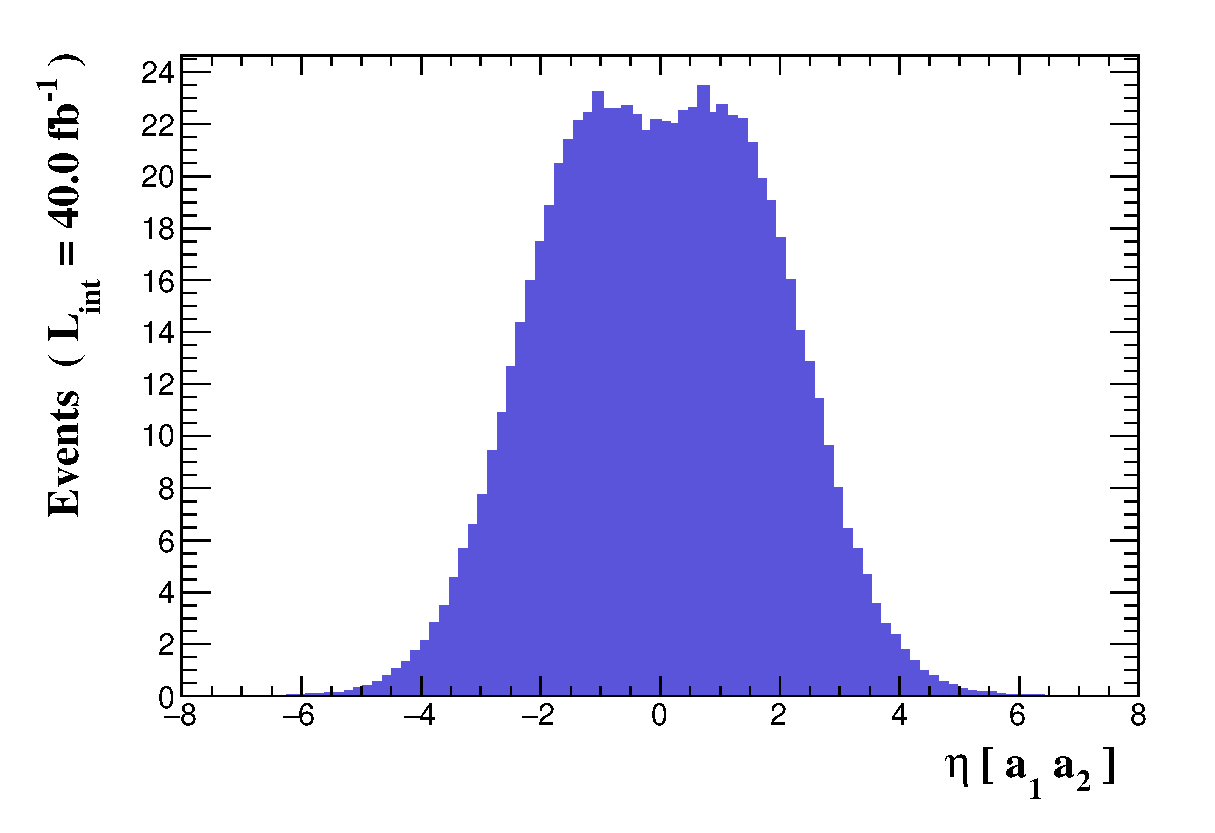
\includegraphics[scale=0.45]{selection_0.eps}\\
\caption{   }
  \end{center}
\end{figure}
      \newpage
\subsection{ Histogram 2}

\textbf{* Plot: ETA ( jets[1] ) }\\
   \begin{table}[H]
  \begin{center}
    \begin{tabular}{|m{23.0mm}|m{23.0mm}|m{18.0mm}|m{19.0mm}|m{19.0mm}|m{19.0mm}|m{19.0mm}|}
      \hline
      {\cellcolor{yellow}         Dataset}& {\cellcolor{yellow}         Integral}& {\cellcolor{yellow}         Entries per event}& {\cellcolor{yellow}         Mean}& {\cellcolor{yellow}         RMS}& {\cellcolor{yellow}         \% underflow}& {\cellcolor{yellow}         \% overflow}\\
      \hline
      {\cellcolor{white}         signal}& {\cellcolor{white}         853}& {\cellcolor{white}         1.0}& {\cellcolor{white}         1.51865}& {\cellcolor{white}         0.8256}& {\cellcolor{green}         0.0}& {\cellcolor{green}         0.0}\\
      \hline
      {\cellcolor{white}         bg\_vbf\_0\_100}& {\cellcolor{white}         102}& {\cellcolor{white}         1.0}& {\cellcolor{white}         3.69767}& {\cellcolor{white}         0.6913}& {\cellcolor{green}         0.0}& {\cellcolor{green}         0.0}\\
      \hline
      {\cellcolor{white}         bg\_vbf\_100\_200}& {\cellcolor{white}         477}& {\cellcolor{white}         1.0}& {\cellcolor{white}         3.05831}& {\cellcolor{white}         0.7484}& {\cellcolor{green}         0.0}& {\cellcolor{green}         0.0}\\
      \hline
      {\cellcolor{white}         bg\_vbf\_200\_400}& {\cellcolor{white}         573}& {\cellcolor{white}         1.0}& {\cellcolor{white}         2.48868}& {\cellcolor{white}         0.7253}& {\cellcolor{green}         0.0}& {\cellcolor{green}         0.0}\\
      \hline
      {\cellcolor{white}         bg\_vbf\_400\_600}& {\cellcolor{white}         174}& {\cellcolor{white}         1.0}& {\cellcolor{white}         1.9668}& {\cellcolor{white}         0.7042}& {\cellcolor{green}         0.0}& {\cellcolor{green}         0.0}\\
      \hline
      {\cellcolor{white}         bg\_vbf\_600\_800}& {\cellcolor{white}         55.7}& {\cellcolor{white}         1.0}& {\cellcolor{white}         1.67633}& {\cellcolor{white}         0.6784}& {\cellcolor{green}         0.0}& {\cellcolor{green}         0.0}\\
      \hline
      {\cellcolor{white}         bg\_vbf\_800\_1200}& {\cellcolor{white}         20.2}& {\cellcolor{white}         1.0}& {\cellcolor{white}         1.56562}& {\cellcolor{white}         0.5919}& {\cellcolor{green}         0.0}& {\cellcolor{green}         0.0}\\
      \hline
      {\cellcolor{white}         bg\_vbf\_1200\_1600}& {\cellcolor{white}         2.25}& {\cellcolor{white}         1.0}& {\cellcolor{white}         1.47431}& {\cellcolor{white}         0.4874}& {\cellcolor{green}         0.0}& {\cellcolor{green}         0.0}\\
      \hline
      {\cellcolor{white}         bg\_vbf\_1600\_inf}& {\cellcolor{white}         0.403}& {\cellcolor{white}         1.0}& {\cellcolor{white}         1.42179}& {\cellcolor{white}         0.4013}& {\cellcolor{green}         0.0}& {\cellcolor{green}         0.0}\\
      \hline
      {\cellcolor{white}         bg\_dip\_0\_100}& {\cellcolor{white}         117}& {\cellcolor{white}         1.0}& {\cellcolor{white}         3.61672}& {\cellcolor{white}         0.8533}& {\cellcolor{green}         0.0}& {\cellcolor{green}         0.0}\\
      \hline
      {\cellcolor{white}         bg\_dip\_100\_200}& {\cellcolor{white}         496}& {\cellcolor{white}         1.0}& {\cellcolor{white}         3.05543}& {\cellcolor{white}         0.9267}& {\cellcolor{green}         0.0}& {\cellcolor{green}         0.0}\\
      \hline
      {\cellcolor{white}         bg\_dip\_200\_400}& {\cellcolor{white}         814}& {\cellcolor{white}         1.0}& {\cellcolor{white}         2.39716}& {\cellcolor{white}         0.8274}& {\cellcolor{green}         0.0}& {\cellcolor{green}         0.0}\\
      \hline
      {\cellcolor{white}         bg\_dip\_400\_600}& {\cellcolor{white}         531}& {\cellcolor{white}         1.0}& {\cellcolor{white}         1.88454}& {\cellcolor{white}         0.7296}& {\cellcolor{green}         0.0}& {\cellcolor{green}         0.0}\\
      \hline
      {\cellcolor{white}         bg\_dip\_600\_800}& {\cellcolor{white}         263}& {\cellcolor{white}         1.0}& {\cellcolor{white}         1.58738}& {\cellcolor{white}         0.6804}& {\cellcolor{green}         0.0}& {\cellcolor{green}         0.0}\\
      \hline
      {\cellcolor{white}         bg\_dip\_800\_1200}& {\cellcolor{white}         96.6}& {\cellcolor{white}         1.0}& {\cellcolor{white}         1.51534}& {\cellcolor{white}         0.5903}& {\cellcolor{green}         0.0}& {\cellcolor{green}         0.0}\\
      \hline
      {\cellcolor{white}         bg\_dip\_1200\_1600}& {\cellcolor{white}         10.8}& {\cellcolor{white}         1.0}& {\cellcolor{white}         1.46872}& {\cellcolor{white}         0.4816}& {\cellcolor{green}         0.0}& {\cellcolor{green}         0.0}\\
      \hline
      {\cellcolor{white}         bg\_dip\_1600\_inf}& {\cellcolor{white}         2.03}& {\cellcolor{white}         1.0}& {\cellcolor{white}         1.4296}& {\cellcolor{white}         0.3873}& {\cellcolor{green}         0.0}& {\cellcolor{green}         0.0}\\
\hline
    \end{tabular}
  \end{center}
\end{table}

\begin{figure}[H]
  \begin{center}
    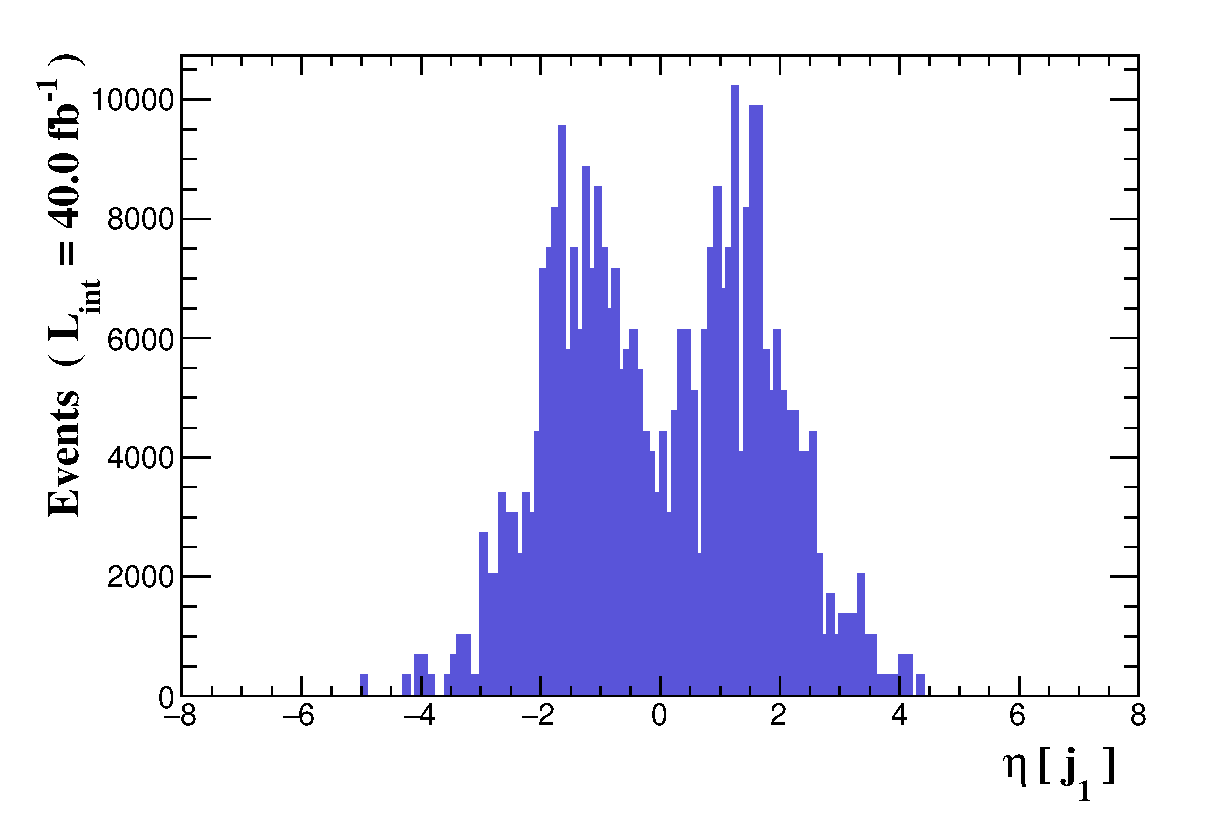
\includegraphics[scale=0.45]{selection_1.eps}\\
\caption{   }
  \end{center}
\end{figure}
      \newpage
\subsection{ Histogram 3}

\textbf{* Plot: PHI ( jets[1] ) }\\
   \begin{table}[H]
  \begin{center}
    \begin{tabular}{|m{23.0mm}|m{23.0mm}|m{18.0mm}|m{19.0mm}|m{19.0mm}|m{19.0mm}|m{19.0mm}|}
      \hline
      {\cellcolor{yellow}         Dataset}& {\cellcolor{yellow}         Integral}& {\cellcolor{yellow}         Entries per event}& {\cellcolor{yellow}         Mean}& {\cellcolor{yellow}         RMS}& {\cellcolor{yellow}         \% underflow}& {\cellcolor{yellow}         \% overflow}\\
      \hline
      {\cellcolor{white}         signal}& {\cellcolor{white}         853}& {\cellcolor{white}         1.0}& {\cellcolor{white}         0.00262009}& {\cellcolor{white}         1.814}& {\cellcolor{green}         0.0}& {\cellcolor{green}         0.0}\\
      \hline
      {\cellcolor{white}         bg\_vbf\_0\_100}& {\cellcolor{white}         102}& {\cellcolor{white}         1.0}& {\cellcolor{white}         -0.00381425}& {\cellcolor{white}         1.809}& {\cellcolor{green}         0.0}& {\cellcolor{green}         0.0}\\
      \hline
      {\cellcolor{white}         bg\_vbf\_100\_200}& {\cellcolor{white}         477}& {\cellcolor{white}         1.0}& {\cellcolor{white}         -0.00399372}& {\cellcolor{white}         1.815}& {\cellcolor{green}         0.0}& {\cellcolor{green}         0.0}\\
      \hline
      {\cellcolor{white}         bg\_vbf\_200\_400}& {\cellcolor{white}         573}& {\cellcolor{white}         1.0}& {\cellcolor{white}         -0.000180864}& {\cellcolor{white}         1.812}& {\cellcolor{green}         0.0}& {\cellcolor{green}         0.0}\\
      \hline
      {\cellcolor{white}         bg\_vbf\_400\_600}& {\cellcolor{white}         174}& {\cellcolor{white}         1.0}& {\cellcolor{white}         -0.0007668}& {\cellcolor{white}         1.812}& {\cellcolor{green}         0.0}& {\cellcolor{green}         0.0}\\
      \hline
      {\cellcolor{white}         bg\_vbf\_600\_800}& {\cellcolor{white}         55.7}& {\cellcolor{white}         1.0}& {\cellcolor{white}         0.000310622}& {\cellcolor{white}         1.814}& {\cellcolor{green}         0.0}& {\cellcolor{green}         0.0}\\
      \hline
      {\cellcolor{white}         bg\_vbf\_800\_1200}& {\cellcolor{white}         20.2}& {\cellcolor{white}         1.0}& {\cellcolor{white}         -0.00826697}& {\cellcolor{white}         1.815}& {\cellcolor{green}         0.0}& {\cellcolor{green}         0.0}\\
      \hline
      {\cellcolor{white}         bg\_vbf\_1200\_1600}& {\cellcolor{white}         2.25}& {\cellcolor{white}         1.0}& {\cellcolor{white}         0.000685286}& {\cellcolor{white}         1.809}& {\cellcolor{green}         0.0}& {\cellcolor{green}         0.0}\\
      \hline
      {\cellcolor{white}         bg\_vbf\_1600\_inf}& {\cellcolor{white}         0.403}& {\cellcolor{white}         1.0}& {\cellcolor{white}         -0.00505461}& {\cellcolor{white}         1.814}& {\cellcolor{green}         0.0}& {\cellcolor{green}         0.0}\\
      \hline
      {\cellcolor{white}         bg\_dip\_0\_100}& {\cellcolor{white}         117}& {\cellcolor{white}         1.0}& {\cellcolor{white}         0.131552}& {\cellcolor{white}         1.932}& {\cellcolor{green}         0.0}& {\cellcolor{green}         0.0}\\
      \hline
      {\cellcolor{white}         bg\_dip\_100\_200}& {\cellcolor{white}         496}& {\cellcolor{white}         1.0}& {\cellcolor{white}         -0.0494161}& {\cellcolor{white}         1.808}& {\cellcolor{green}         0.0}& {\cellcolor{green}         0.0}\\
      \hline
      {\cellcolor{white}         bg\_dip\_200\_400}& {\cellcolor{white}         814}& {\cellcolor{white}         1.0}& {\cellcolor{white}         -0.0325304}& {\cellcolor{white}         1.8}& {\cellcolor{green}         0.0}& {\cellcolor{green}         0.0}\\
      \hline
      {\cellcolor{white}         bg\_dip\_400\_600}& {\cellcolor{white}         531}& {\cellcolor{white}         1.0}& {\cellcolor{white}         -0.0180546}& {\cellcolor{white}         1.805}& {\cellcolor{green}         0.0}& {\cellcolor{green}         0.0}\\
      \hline
      {\cellcolor{white}         bg\_dip\_600\_800}& {\cellcolor{white}         263}& {\cellcolor{white}         1.0}& {\cellcolor{white}         -0.00294976}& {\cellcolor{white}         1.824}& {\cellcolor{green}         0.0}& {\cellcolor{green}         0.0}\\
      \hline
      {\cellcolor{white}         bg\_dip\_800\_1200}& {\cellcolor{white}         96.6}& {\cellcolor{white}         1.0}& {\cellcolor{white}         0.00642014}& {\cellcolor{white}         1.813}& {\cellcolor{green}         0.0}& {\cellcolor{green}         0.0}\\
      \hline
      {\cellcolor{white}         bg\_dip\_1200\_1600}& {\cellcolor{white}         10.8}& {\cellcolor{white}         1.0}& {\cellcolor{white}         0.00301387}& {\cellcolor{white}         1.825}& {\cellcolor{green}         0.0}& {\cellcolor{green}         0.0}\\
      \hline
      {\cellcolor{white}         bg\_dip\_1600\_inf}& {\cellcolor{white}         2.03}& {\cellcolor{white}         1.0}& {\cellcolor{white}         -0.0114902}& {\cellcolor{white}         1.816}& {\cellcolor{green}         0.0}& {\cellcolor{green}         0.0}\\
\hline
    \end{tabular}
  \end{center}
\end{table}

\begin{figure}[H]
  \begin{center}
    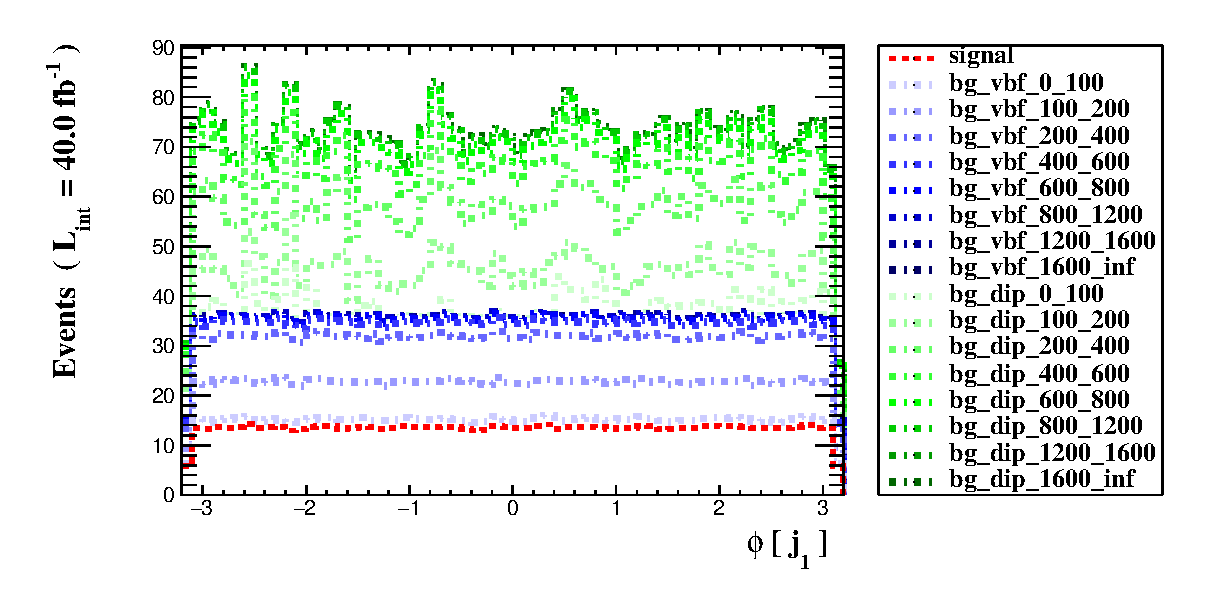
\includegraphics[scale=0.45]{selection_2.eps}\\
\caption{   }
  \end{center}
\end{figure}
      \newpage
\subsection{ Histogram 4}

\textbf{* Plot: PT ( jets[2] ) }\\
   \begin{table}[H]
  \begin{center}
    \begin{tabular}{|m{23.0mm}|m{23.0mm}|m{18.0mm}|m{19.0mm}|m{19.0mm}|m{19.0mm}|m{19.0mm}|}
      \hline
      {\cellcolor{yellow}         Dataset}& {\cellcolor{yellow}         Integral}& {\cellcolor{yellow}         Entries per event}& {\cellcolor{yellow}         Mean}& {\cellcolor{yellow}         RMS}& {\cellcolor{yellow}         \% underflow}& {\cellcolor{yellow}         \% overflow}\\
      \hline
      {\cellcolor{white}         signal}& {\cellcolor{white}         853}& {\cellcolor{white}         1.0}& {\cellcolor{white}         205.725}& {\cellcolor{white}         143.1}& {\cellcolor{green}         0.0}& {\cellcolor{green}         4.097}\\
      \hline
      {\cellcolor{white}         bg\_vbf\_0\_100}& {\cellcolor{white}         102}& {\cellcolor{white}         1.0}& {\cellcolor{white}         32.1093}& {\cellcolor{white}         7.26}& {\cellcolor{green}         0.0}& {\cellcolor{green}         0.0}\\
      \hline
      {\cellcolor{white}         bg\_vbf\_100\_200}& {\cellcolor{white}         477}& {\cellcolor{white}         1.0}& {\cellcolor{white}         59.3482}& {\cellcolor{white}         16.86}& {\cellcolor{green}         0.0}& {\cellcolor{green}         0.0}\\
      \hline
      {\cellcolor{white}         bg\_vbf\_200\_400}& {\cellcolor{white}         573}& {\cellcolor{white}         1.0}& {\cellcolor{white}         115.402}& {\cellcolor{white}         33.11}& {\cellcolor{green}         0.0}& {\cellcolor{green}         0.0}\\
      \hline
      {\cellcolor{white}         bg\_vbf\_400\_600}& {\cellcolor{white}         174}& {\cellcolor{white}         1.0}& {\cellcolor{white}         203.446}& {\cellcolor{white}         46.93}& {\cellcolor{green}         0.0}& {\cellcolor{green}         0.0}\\
      \hline
      {\cellcolor{white}         bg\_vbf\_600\_800}& {\cellcolor{white}         55.7}& {\cellcolor{white}         1.0}& {\cellcolor{white}         291.584}& {\cellcolor{white}         61.32}& {\cellcolor{green}         0.0}& {\cellcolor{green}         0.0}\\
      \hline
      {\cellcolor{white}         bg\_vbf\_800\_1200}& {\cellcolor{white}         20.2}& {\cellcolor{white}         1.0}& {\cellcolor{white}         401.508}& {\cellcolor{white}         94.51}& {\cellcolor{orange}         0.0}& {\cellcolor{orange}         11.67}\\
      \hline
      {\cellcolor{white}         bg\_vbf\_1200\_1600}& {\cellcolor{white}         2.25}& {\cellcolor{white}         1.0}& {\cellcolor{white}         591.301}& {\cellcolor{white}         126.8}& {\cellcolor{red}         0.0}& {\cellcolor{red}         86.39}\\
      \hline
      {\cellcolor{white}         bg\_vbf\_1600\_inf}& {\cellcolor{white}         0.403}& {\cellcolor{white}         1.0}& {\cellcolor{white}         825.305}& {\cellcolor{white}         181.1}& {\cellcolor{red}         0.0}& {\cellcolor{red}         95.2}\\
      \hline
      {\cellcolor{white}         bg\_dip\_0\_100}& {\cellcolor{white}         117}& {\cellcolor{white}         1.0}& {\cellcolor{white}         32.1082}& {\cellcolor{white}         6.852}& {\cellcolor{green}         0.0}& {\cellcolor{green}         0.0}\\
      \hline
      {\cellcolor{white}         bg\_dip\_100\_200}& {\cellcolor{white}         496}& {\cellcolor{white}         1.0}& {\cellcolor{white}         58.8617}& {\cellcolor{white}         17.59}& {\cellcolor{green}         0.0}& {\cellcolor{green}         0.0}\\
      \hline
      {\cellcolor{white}         bg\_dip\_200\_400}& {\cellcolor{white}         814}& {\cellcolor{white}         1.0}& {\cellcolor{white}         119.32}& {\cellcolor{white}         37.13}& {\cellcolor{green}         0.0}& {\cellcolor{green}         0.0}\\
      \hline
      {\cellcolor{white}         bg\_dip\_400\_600}& {\cellcolor{white}         531}& {\cellcolor{white}         1.0}& {\cellcolor{white}         214.002}& {\cellcolor{white}         47.08}& {\cellcolor{green}         0.0}& {\cellcolor{green}         0.0}\\
      \hline
      {\cellcolor{white}         bg\_dip\_600\_800}& {\cellcolor{white}         263}& {\cellcolor{white}         1.0}& {\cellcolor{white}         302.138}& {\cellcolor{white}         53.94}& {\cellcolor{green}         0.0}& {\cellcolor{green}         0.0}\\
      \hline
      {\cellcolor{white}         bg\_dip\_800\_1200}& {\cellcolor{white}         96.6}& {\cellcolor{white}         1.0}& {\cellcolor{white}         414.316}& {\cellcolor{white}         87.72}& {\cellcolor{orange}         0.0}& {\cellcolor{orange}         13.24}\\
      \hline
      {\cellcolor{white}         bg\_dip\_1200\_1600}& {\cellcolor{white}         10.8}& {\cellcolor{white}         1.0}& {\cellcolor{white}         610.588}& {\cellcolor{white}         111.8}& {\cellcolor{red}         0.0}& {\cellcolor{red}         91.98}\\
      \hline
      {\cellcolor{white}         bg\_dip\_1600\_inf}& {\cellcolor{white}         2.03}& {\cellcolor{white}         1.0}& {\cellcolor{white}         856.028}& {\cellcolor{white}         157.0}& {\cellcolor{red}         0.0}& {\cellcolor{red}         98.0}\\
\hline
    \end{tabular}
  \end{center}
\end{table}

\begin{figure}[H]
  \begin{center}
    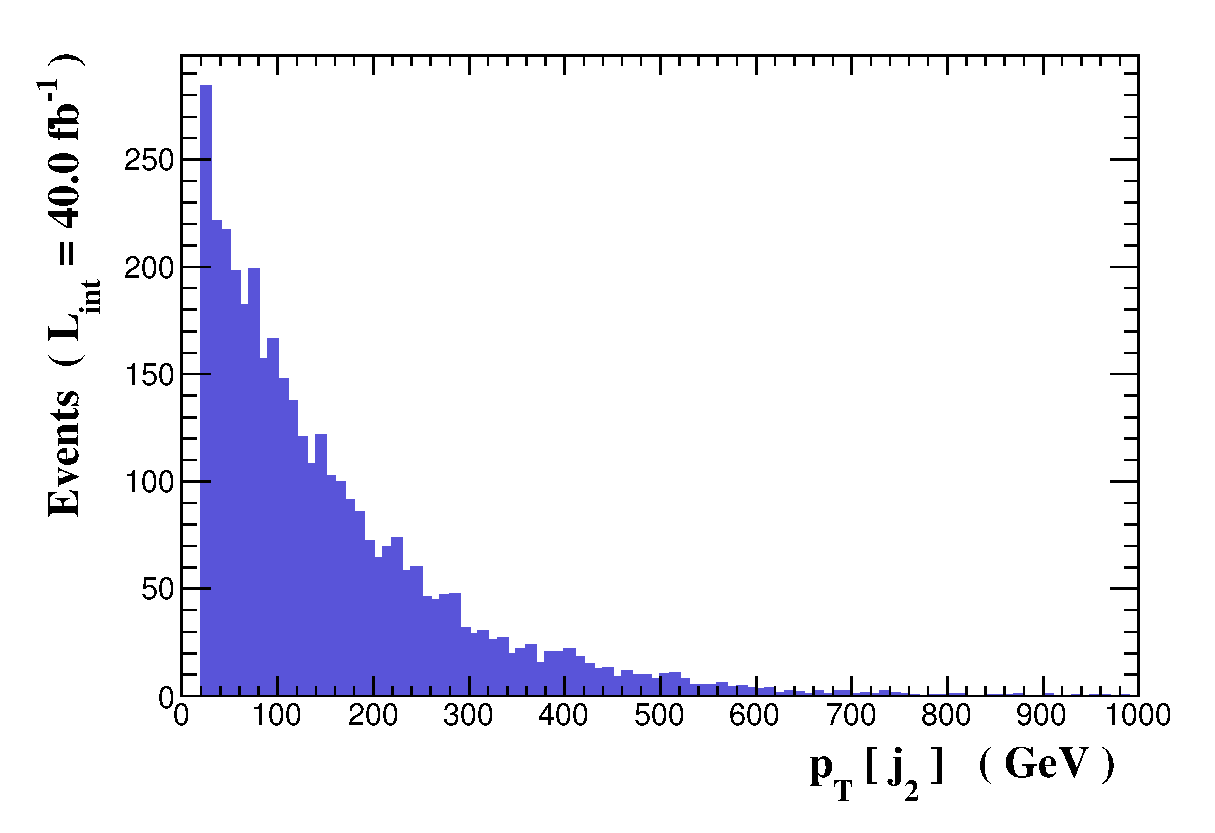
\includegraphics[scale=0.45]{selection_3.eps}\\
\caption{   }
  \end{center}
\end{figure}
      \newpage
\subsection{ Histogram 5}

\textbf{* Plot: ETA ( jets[2] ) }\\
   \begin{table}[H]
  \begin{center}
    \begin{tabular}{|m{23.0mm}|m{23.0mm}|m{18.0mm}|m{19.0mm}|m{19.0mm}|m{19.0mm}|m{19.0mm}|}
      \hline
      {\cellcolor{yellow}         Dataset}& {\cellcolor{yellow}         Integral}& {\cellcolor{yellow}         Entries per event}& {\cellcolor{yellow}         Mean}& {\cellcolor{yellow}         RMS}& {\cellcolor{yellow}         \% underflow}& {\cellcolor{yellow}         \% overflow}\\
      \hline
      {\cellcolor{white}         signal}& {\cellcolor{white}         853}& {\cellcolor{white}         1.0}& {\cellcolor{white}         -2.41853}& {\cellcolor{white}         0.9021}& {\cellcolor{green}         0.0}& {\cellcolor{green}         0.0}\\
      \hline
      {\cellcolor{white}         bg\_vbf\_0\_100}& {\cellcolor{white}         102}& {\cellcolor{white}         1.0}& {\cellcolor{white}         -3.87669}& {\cellcolor{white}         0.6852}& {\cellcolor{green}         0.0}& {\cellcolor{green}         0.0}\\
      \hline
      {\cellcolor{white}         bg\_vbf\_100\_200}& {\cellcolor{white}         477}& {\cellcolor{white}         1.0}& {\cellcolor{white}         -3.34195}& {\cellcolor{white}         0.7753}& {\cellcolor{green}         0.0}& {\cellcolor{green}         0.0}\\
      \hline
      {\cellcolor{white}         bg\_vbf\_200\_400}& {\cellcolor{white}         573}& {\cellcolor{white}         1.0}& {\cellcolor{white}         -2.76309}& {\cellcolor{white}         0.7681}& {\cellcolor{green}         0.0}& {\cellcolor{green}         0.0}\\
      \hline
      {\cellcolor{white}         bg\_vbf\_400\_600}& {\cellcolor{white}         174}& {\cellcolor{white}         1.0}& {\cellcolor{white}         -2.21601}& {\cellcolor{white}         0.7459}& {\cellcolor{green}         0.0}& {\cellcolor{green}         0.0}\\
      \hline
      {\cellcolor{white}         bg\_vbf\_600\_800}& {\cellcolor{white}         55.7}& {\cellcolor{white}         1.0}& {\cellcolor{white}         -1.90089}& {\cellcolor{white}         0.7218}& {\cellcolor{green}         0.0}& {\cellcolor{green}         0.0}\\
      \hline
      {\cellcolor{white}         bg\_vbf\_800\_1200}& {\cellcolor{white}         20.2}& {\cellcolor{white}         1.0}& {\cellcolor{white}         -1.79372}& {\cellcolor{white}         0.6283}& {\cellcolor{green}         0.0}& {\cellcolor{green}         0.0}\\
      \hline
      {\cellcolor{white}         bg\_vbf\_1200\_1600}& {\cellcolor{white}         2.25}& {\cellcolor{white}         1.0}& {\cellcolor{white}         -1.67073}& {\cellcolor{white}         0.5231}& {\cellcolor{green}         0.0}& {\cellcolor{green}         0.0}\\
      \hline
      {\cellcolor{white}         bg\_vbf\_1600\_inf}& {\cellcolor{white}         0.403}& {\cellcolor{white}         1.0}& {\cellcolor{white}         -1.58018}& {\cellcolor{white}         0.4338}& {\cellcolor{green}         0.0}& {\cellcolor{green}         0.0}\\
      \hline
      {\cellcolor{white}         bg\_dip\_0\_100}& {\cellcolor{white}         117}& {\cellcolor{white}         1.0}& {\cellcolor{white}         -3.69603}& {\cellcolor{white}         0.8703}& {\cellcolor{green}         0.0}& {\cellcolor{green}         0.0}\\
      \hline
      {\cellcolor{white}         bg\_dip\_100\_200}& {\cellcolor{white}         496}& {\cellcolor{white}         1.0}& {\cellcolor{white}         -3.05582}& {\cellcolor{white}         0.9476}& {\cellcolor{green}         0.0}& {\cellcolor{green}         0.0}\\
      \hline
      {\cellcolor{white}         bg\_dip\_200\_400}& {\cellcolor{white}         814}& {\cellcolor{white}         1.0}& {\cellcolor{white}         -2.42149}& {\cellcolor{white}         0.9066}& {\cellcolor{green}         0.0}& {\cellcolor{green}         0.0}\\
      \hline
      {\cellcolor{white}         bg\_dip\_400\_600}& {\cellcolor{white}         531}& {\cellcolor{white}         1.0}& {\cellcolor{white}         -1.84889}& {\cellcolor{white}         0.7917}& {\cellcolor{green}         0.0}& {\cellcolor{green}         0.0}\\
      \hline
      {\cellcolor{white}         bg\_dip\_600\_800}& {\cellcolor{white}         263}& {\cellcolor{white}         1.0}& {\cellcolor{white}         -1.58425}& {\cellcolor{white}         0.7171}& {\cellcolor{green}         0.0}& {\cellcolor{green}         0.0}\\
      \hline
      {\cellcolor{white}         bg\_dip\_800\_1200}& {\cellcolor{white}         96.6}& {\cellcolor{white}         1.0}& {\cellcolor{white}         -1.56186}& {\cellcolor{white}         0.6304}& {\cellcolor{green}         0.0}& {\cellcolor{green}         0.0}\\
      \hline
      {\cellcolor{white}         bg\_dip\_1200\_1600}& {\cellcolor{white}         10.8}& {\cellcolor{white}         1.0}& {\cellcolor{white}         -1.51945}& {\cellcolor{white}         0.5189}& {\cellcolor{green}         0.0}& {\cellcolor{green}         0.0}\\
      \hline
      {\cellcolor{white}         bg\_dip\_1600\_inf}& {\cellcolor{white}         2.03}& {\cellcolor{white}         1.0}& {\cellcolor{white}         -1.47137}& {\cellcolor{white}         0.4096}& {\cellcolor{green}         0.0}& {\cellcolor{green}         0.0}\\
\hline
    \end{tabular}
  \end{center}
\end{table}

\begin{figure}[H]
  \begin{center}
    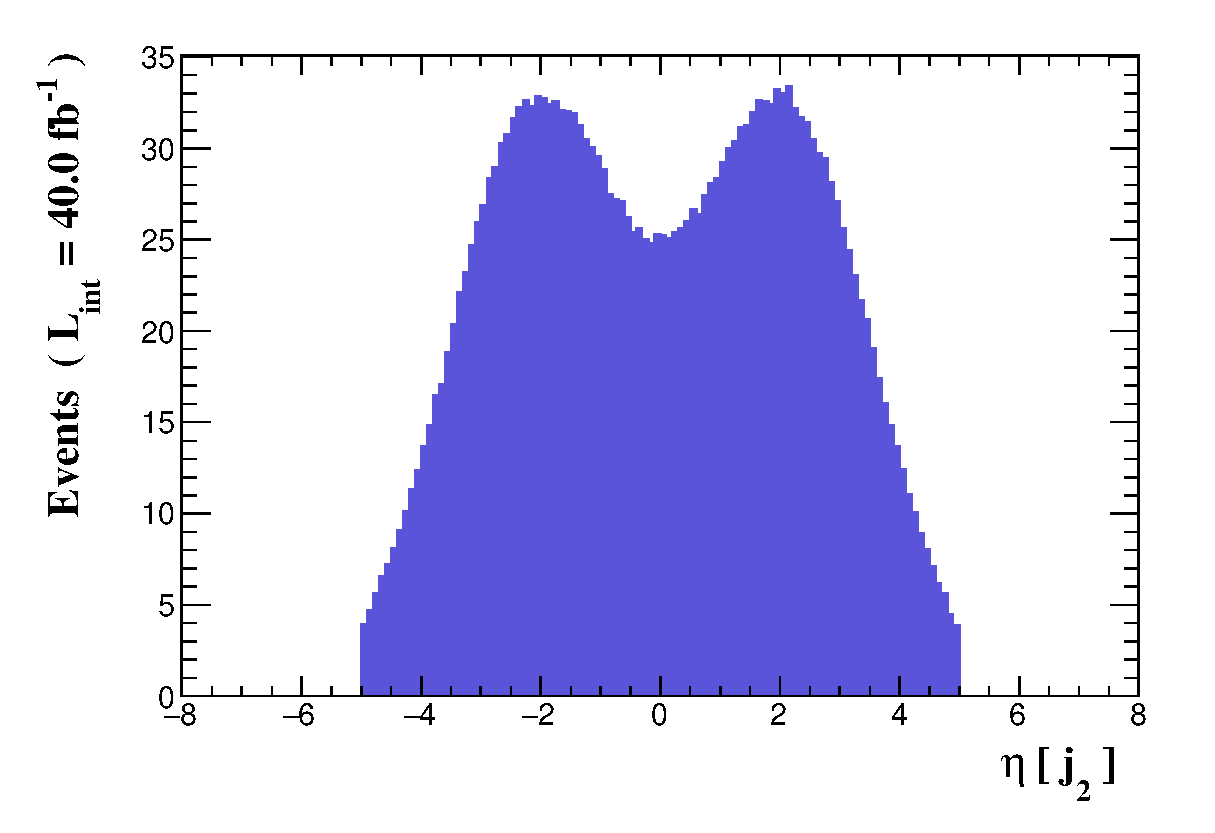
\includegraphics[scale=0.45]{selection_4.eps}\\
\caption{   }
  \end{center}
\end{figure}
      \newpage
\subsection{ Histogram 6}

\textbf{* Plot: PHI ( jets[2] ) }\\
   \begin{table}[H]
  \begin{center}
    \begin{tabular}{|m{23.0mm}|m{23.0mm}|m{18.0mm}|m{19.0mm}|m{19.0mm}|m{19.0mm}|m{19.0mm}|}
      \hline
      {\cellcolor{yellow}         Dataset}& {\cellcolor{yellow}         Integral}& {\cellcolor{yellow}         Entries per event}& {\cellcolor{yellow}         Mean}& {\cellcolor{yellow}         RMS}& {\cellcolor{yellow}         \% underflow}& {\cellcolor{yellow}         \% overflow}\\
      \hline
      {\cellcolor{white}         signal}& {\cellcolor{white}         853}& {\cellcolor{white}         1.0}& {\cellcolor{white}         -0.00548129}& {\cellcolor{white}         1.812}& {\cellcolor{green}         0.0}& {\cellcolor{green}         0.0}\\
      \hline
      {\cellcolor{white}         bg\_vbf\_0\_100}& {\cellcolor{white}         102}& {\cellcolor{white}         1.0}& {\cellcolor{white}         -0.0109881}& {\cellcolor{white}         1.822}& {\cellcolor{green}         0.0}& {\cellcolor{green}         0.0}\\
      \hline
      {\cellcolor{white}         bg\_vbf\_100\_200}& {\cellcolor{white}         477}& {\cellcolor{white}         1.0}& {\cellcolor{white}         0.00648616}& {\cellcolor{white}         1.818}& {\cellcolor{green}         0.0}& {\cellcolor{green}         0.0}\\
      \hline
      {\cellcolor{white}         bg\_vbf\_200\_400}& {\cellcolor{white}         573}& {\cellcolor{white}         1.0}& {\cellcolor{white}         -0.000152277}& {\cellcolor{white}         1.815}& {\cellcolor{green}         0.0}& {\cellcolor{green}         0.0}\\
      \hline
      {\cellcolor{white}         bg\_vbf\_400\_600}& {\cellcolor{white}         174}& {\cellcolor{white}         1.0}& {\cellcolor{white}         -0.000896361}& {\cellcolor{white}         1.816}& {\cellcolor{green}         0.0}& {\cellcolor{green}         0.0}\\
      \hline
      {\cellcolor{white}         bg\_vbf\_600\_800}& {\cellcolor{white}         55.7}& {\cellcolor{white}         1.0}& {\cellcolor{white}         0.00247374}& {\cellcolor{white}         1.814}& {\cellcolor{green}         0.0}& {\cellcolor{green}         0.0}\\
      \hline
      {\cellcolor{white}         bg\_vbf\_800\_1200}& {\cellcolor{white}         20.2}& {\cellcolor{white}         1.0}& {\cellcolor{white}         -0.000887017}& {\cellcolor{white}         1.81}& {\cellcolor{green}         0.0}& {\cellcolor{green}         0.0}\\
      \hline
      {\cellcolor{white}         bg\_vbf\_1200\_1600}& {\cellcolor{white}         2.25}& {\cellcolor{white}         1.0}& {\cellcolor{white}         -0.0022585}& {\cellcolor{white}         1.82}& {\cellcolor{green}         0.0}& {\cellcolor{green}         0.0}\\
      \hline
      {\cellcolor{white}         bg\_vbf\_1600\_inf}& {\cellcolor{white}         0.403}& {\cellcolor{white}         1.0}& {\cellcolor{white}         0.0107912}& {\cellcolor{white}         1.808}& {\cellcolor{green}         0.0}& {\cellcolor{green}         0.0}\\
      \hline
      {\cellcolor{white}         bg\_dip\_0\_100}& {\cellcolor{white}         117}& {\cellcolor{white}         1.0}& {\cellcolor{white}         -0.382442}& {\cellcolor{white}         1.517}& {\cellcolor{green}         0.0}& {\cellcolor{green}         0.0}\\
      \hline
      {\cellcolor{white}         bg\_dip\_100\_200}& {\cellcolor{white}         496}& {\cellcolor{white}         1.0}& {\cellcolor{white}         0.0518113}& {\cellcolor{white}         1.834}& {\cellcolor{green}         0.0}& {\cellcolor{green}         0.0}\\
      \hline
      {\cellcolor{white}         bg\_dip\_200\_400}& {\cellcolor{white}         814}& {\cellcolor{white}         1.0}& {\cellcolor{white}         -0.013668}& {\cellcolor{white}         1.825}& {\cellcolor{green}         0.0}& {\cellcolor{green}         0.0}\\
      \hline
      {\cellcolor{white}         bg\_dip\_400\_600}& {\cellcolor{white}         531}& {\cellcolor{white}         1.0}& {\cellcolor{white}         -0.0091491}& {\cellcolor{white}         1.822}& {\cellcolor{green}         0.0}& {\cellcolor{green}         0.0}\\
      \hline
      {\cellcolor{white}         bg\_dip\_600\_800}& {\cellcolor{white}         263}& {\cellcolor{white}         1.0}& {\cellcolor{white}         -0.0115319}& {\cellcolor{white}         1.804}& {\cellcolor{green}         0.0}& {\cellcolor{green}         0.0}\\
      \hline
      {\cellcolor{white}         bg\_dip\_800\_1200}& {\cellcolor{white}         96.6}& {\cellcolor{white}         1.0}& {\cellcolor{white}         -0.00818692}& {\cellcolor{white}         1.814}& {\cellcolor{green}         0.0}& {\cellcolor{green}         0.0}\\
      \hline
      {\cellcolor{white}         bg\_dip\_1200\_1600}& {\cellcolor{white}         10.8}& {\cellcolor{white}         1.0}& {\cellcolor{white}         0.0189346}& {\cellcolor{white}         1.8}& {\cellcolor{green}         0.0}& {\cellcolor{green}         0.0}\\
      \hline
      {\cellcolor{white}         bg\_dip\_1600\_inf}& {\cellcolor{white}         2.03}& {\cellcolor{white}         1.0}& {\cellcolor{white}         -0.000887935}& {\cellcolor{white}         1.813}& {\cellcolor{green}         0.0}& {\cellcolor{green}         0.0}\\
\hline
    \end{tabular}
  \end{center}
\end{table}

\begin{figure}[H]
  \begin{center}
    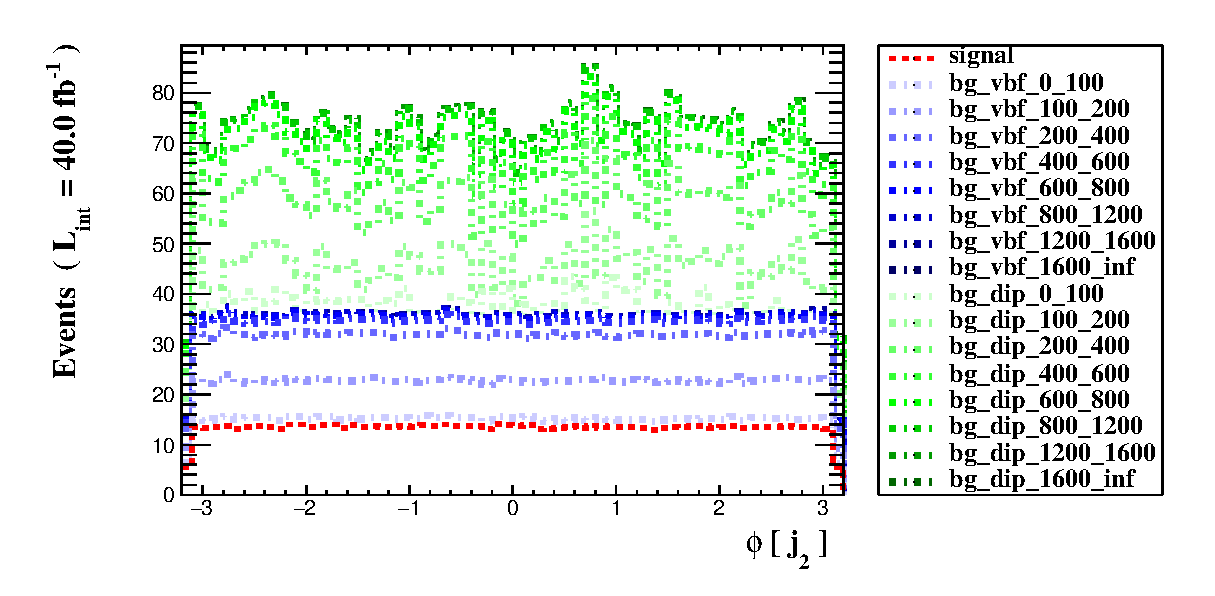
\includegraphics[scale=0.45]{selection_5.eps}\\
\caption{   }
  \end{center}
\end{figure}
      \newpage
\subsection{ Histogram 7}

\textbf{* Plot: DELTAR ( jets[1] , jets[2] ) }\\
   \begin{table}[H]
  \begin{center}
    \begin{tabular}{|m{23.0mm}|m{23.0mm}|m{18.0mm}|m{19.0mm}|m{19.0mm}|m{19.0mm}|m{19.0mm}|}
      \hline
      {\cellcolor{yellow}         Dataset}& {\cellcolor{yellow}         Integral}& {\cellcolor{yellow}         Entries per event}& {\cellcolor{yellow}         Mean}& {\cellcolor{yellow}         RMS}& {\cellcolor{yellow}         \% underflow}& {\cellcolor{yellow}         \% overflow}\\
      \hline
      {\cellcolor{white}         signal}& {\cellcolor{white}         853}& {\cellcolor{white}         1.0}& {\cellcolor{white}         4.42115}& {\cellcolor{white}         1.166}& {\cellcolor{green}         0.0}& {\cellcolor{green}         0.0}\\
      \hline
      {\cellcolor{white}         bg\_vbf\_0\_100}& {\cellcolor{white}         102}& {\cellcolor{white}         1.0}& {\cellcolor{white}         7.95218}& {\cellcolor{white}         0.591}& {\cellcolor{green}         0.0}& {\cellcolor{green}         0.0}\\
      \hline
      {\cellcolor{white}         bg\_vbf\_100\_200}& {\cellcolor{white}         477}& {\cellcolor{white}         1.0}& {\cellcolor{white}         6.93039}& {\cellcolor{white}         0.6173}& {\cellcolor{green}         0.0}& {\cellcolor{green}         0.0}\\
      \hline
      {\cellcolor{white}         bg\_vbf\_200\_400}& {\cellcolor{white}         573}& {\cellcolor{white}         1.0}& {\cellcolor{white}         5.94197}& {\cellcolor{white}         0.6418}& {\cellcolor{green}         0.0}& {\cellcolor{green}         0.0}\\
      \hline
      {\cellcolor{white}         bg\_vbf\_400\_600}& {\cellcolor{white}         174}& {\cellcolor{white}         1.0}& {\cellcolor{white}         5.06636}& {\cellcolor{white}         0.595}& {\cellcolor{green}         0.0}& {\cellcolor{green}         0.0}\\
      \hline
      {\cellcolor{white}         bg\_vbf\_600\_800}& {\cellcolor{white}         55.7}& {\cellcolor{white}         1.0}& {\cellcolor{white}         4.61037}& {\cellcolor{white}         0.5519}& {\cellcolor{green}         0.0}& {\cellcolor{green}         0.0}\\
      \hline
      {\cellcolor{white}         bg\_vbf\_800\_1200}& {\cellcolor{white}         20.2}& {\cellcolor{white}         1.0}& {\cellcolor{white}         4.45532}& {\cellcolor{white}         0.4696}& {\cellcolor{green}         0.0}& {\cellcolor{green}         0.0}\\
      \hline
      {\cellcolor{white}         bg\_vbf\_1200\_1600}& {\cellcolor{white}         2.25}& {\cellcolor{white}         1.0}& {\cellcolor{white}         4.32176}& {\cellcolor{white}         0.3646}& {\cellcolor{green}         0.0}& {\cellcolor{green}         0.0}\\
      \hline
      {\cellcolor{white}         bg\_vbf\_1600\_inf}& {\cellcolor{white}         0.403}& {\cellcolor{white}         1.0}& {\cellcolor{white}         4.24682}& {\cellcolor{white}         0.289}& {\cellcolor{green}         0.0}& {\cellcolor{green}         0.0}\\
      \hline
      {\cellcolor{white}         bg\_dip\_0\_100}& {\cellcolor{white}         117}& {\cellcolor{white}         1.0}& {\cellcolor{white}         7.74752}& {\cellcolor{white}         0.3267}& {\cellcolor{green}         0.0}& {\cellcolor{green}         0.0}\\
      \hline
      {\cellcolor{white}         bg\_dip\_100\_200}& {\cellcolor{white}         496}& {\cellcolor{white}         1.0}& {\cellcolor{white}         6.66929}& {\cellcolor{white}         0.4759}& {\cellcolor{green}         0.0}& {\cellcolor{green}         0.0}\\
      \hline
      {\cellcolor{white}         bg\_dip\_200\_400}& {\cellcolor{white}         814}& {\cellcolor{white}         1.0}& {\cellcolor{white}         5.59206}& {\cellcolor{white}         0.4871}& {\cellcolor{green}         0.0}& {\cellcolor{green}         0.0}\\
      \hline
      {\cellcolor{white}         bg\_dip\_400\_600}& {\cellcolor{white}         531}& {\cellcolor{white}         1.0}& {\cellcolor{white}         4.75718}& {\cellcolor{white}         0.4185}& {\cellcolor{green}         0.0}& {\cellcolor{green}         0.0}\\
      \hline
      {\cellcolor{white}         bg\_dip\_600\_800}& {\cellcolor{white}         263}& {\cellcolor{white}         1.0}& {\cellcolor{white}         4.35595}& {\cellcolor{white}         0.3723}& {\cellcolor{green}         0.0}& {\cellcolor{green}         0.0}\\
      \hline
      {\cellcolor{white}         bg\_dip\_800\_1200}& {\cellcolor{white}         96.6}& {\cellcolor{white}         1.0}& {\cellcolor{white}         4.29607}& {\cellcolor{white}         0.3328}& {\cellcolor{green}         0.0}& {\cellcolor{green}         0.0}\\
      \hline
      {\cellcolor{white}         bg\_dip\_1200\_1600}& {\cellcolor{white}         10.8}& {\cellcolor{white}         1.0}& {\cellcolor{white}         4.2533}& {\cellcolor{white}         0.2769}& {\cellcolor{green}         0.0}& {\cellcolor{green}         0.0}\\
      \hline
      {\cellcolor{white}         bg\_dip\_1600\_inf}& {\cellcolor{white}         2.03}& {\cellcolor{white}         1.0}& {\cellcolor{white}         4.21455}& {\cellcolor{white}         0.215}& {\cellcolor{green}         0.0}& {\cellcolor{green}         0.0}\\
\hline
    \end{tabular}
  \end{center}
\end{table}

\begin{figure}[H]
  \begin{center}
    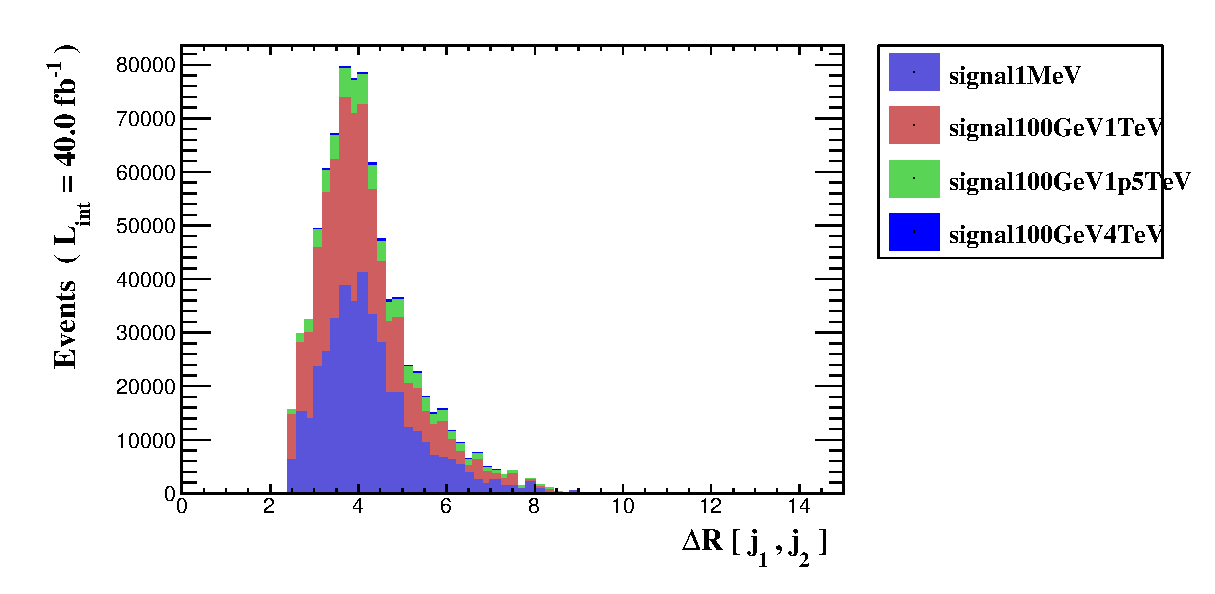
\includegraphics[scale=0.45]{selection_6.eps}\\
\caption{   }
  \end{center}
\end{figure}
      \newpage
\subsection{ Histogram 8}

\textbf{* Plot: M ( jets[1] jets[2] ) }\\
   \begin{table}[H]
  \begin{center}
    \begin{tabular}{|m{23.0mm}|m{23.0mm}|m{18.0mm}|m{19.0mm}|m{19.0mm}|m{19.0mm}|m{19.0mm}|}
      \hline
      {\cellcolor{yellow}         Dataset}& {\cellcolor{yellow}         Integral}& {\cellcolor{yellow}         Entries per event}& {\cellcolor{yellow}         Mean}& {\cellcolor{yellow}         RMS}& {\cellcolor{yellow}         \% underflow}& {\cellcolor{yellow}         \% overflow}\\
      \hline
      {\cellcolor{white}         signal}& {\cellcolor{white}         853}& {\cellcolor{white}         1.0}& {\cellcolor{white}         1998.75}& {\cellcolor{white}         664.8}& {\cellcolor{green}         0.0}& {\cellcolor{green}         0.0}\\
      \hline
      {\cellcolor{white}         bg\_vbf\_0\_100}& {\cellcolor{white}         102}& {\cellcolor{white}         1.0}& {\cellcolor{white}         1754.92}& {\cellcolor{white}         545.8}& {\cellcolor{green}         0.0}& {\cellcolor{green}         0.0}\\
      \hline
      {\cellcolor{white}         bg\_vbf\_100\_200}& {\cellcolor{white}         477}& {\cellcolor{white}         1.0}& {\cellcolor{white}         1797.03}& {\cellcolor{white}         586.5}& {\cellcolor{green}         0.0}& {\cellcolor{green}         0.0}\\
      \hline
      {\cellcolor{white}         bg\_vbf\_200\_400}& {\cellcolor{white}         573}& {\cellcolor{white}         1.0}& {\cellcolor{white}         1935.01}& {\cellcolor{white}         656.1}& {\cellcolor{green}         0.0}& {\cellcolor{green}         0.0}\\
      \hline
      {\cellcolor{white}         bg\_vbf\_400\_600}& {\cellcolor{white}         174}& {\cellcolor{white}         1.0}& {\cellcolor{white}         2014.63}& {\cellcolor{white}         731.2}& {\cellcolor{green}         0.0}& {\cellcolor{green}         0.001131}\\
      \hline
      {\cellcolor{white}         bg\_vbf\_600\_800}& {\cellcolor{white}         55.7}& {\cellcolor{white}         1.0}& {\cellcolor{white}         2138.11}& {\cellcolor{white}         768.7}& {\cellcolor{green}         0.0}& {\cellcolor{green}         0.00317}\\
      \hline
      {\cellcolor{white}         bg\_vbf\_800\_1200}& {\cellcolor{white}         20.2}& {\cellcolor{white}         1.0}& {\cellcolor{white}         2585.16}& {\cellcolor{white}         786.6}& {\cellcolor{green}         0.0}& {\cellcolor{green}         0.007109}\\
      \hline
      {\cellcolor{white}         bg\_vbf\_1200\_1600}& {\cellcolor{white}         2.25}& {\cellcolor{white}         1.0}& {\cellcolor{white}         3328.08}& {\cellcolor{white}         768.0}& {\cellcolor{green}         0.0}& {\cellcolor{green}         0.01539}\\
      \hline
      {\cellcolor{white}         bg\_vbf\_1600\_inf}& {\cellcolor{white}         0.403}& {\cellcolor{white}         1.0}& {\cellcolor{white}         4223.33}& {\cellcolor{white}         831.2}& {\cellcolor{green}         0.0}& {\cellcolor{green}         0.09855}\\
      \hline
      {\cellcolor{white}         bg\_dip\_0\_100}& {\cellcolor{white}         117}& {\cellcolor{white}         1.0}& {\cellcolor{white}         1536.49}& {\cellcolor{white}         260.9}& {\cellcolor{green}         0.0}& {\cellcolor{green}         0.0}\\
      \hline
      {\cellcolor{white}         bg\_dip\_100\_200}& {\cellcolor{white}         496}& {\cellcolor{white}         1.0}& {\cellcolor{white}         1527.46}& {\cellcolor{white}         316.0}& {\cellcolor{green}         0.0}& {\cellcolor{green}         0.0}\\
      \hline
      {\cellcolor{white}         bg\_dip\_200\_400}& {\cellcolor{white}         814}& {\cellcolor{white}         1.0}& {\cellcolor{white}         1563.67}& {\cellcolor{white}         323.6}& {\cellcolor{green}         0.0}& {\cellcolor{green}         0.0}\\
      \hline
      {\cellcolor{white}         bg\_dip\_400\_600}& {\cellcolor{white}         531}& {\cellcolor{white}         1.0}& {\cellcolor{white}         1613.17}& {\cellcolor{white}         379.0}& {\cellcolor{green}         0.0}& {\cellcolor{green}         0.0}\\
      \hline
      {\cellcolor{white}         bg\_dip\_600\_800}& {\cellcolor{white}         263}& {\cellcolor{white}         1.0}& {\cellcolor{white}         1735.66}& {\cellcolor{white}         437.1}& {\cellcolor{green}         0.0}& {\cellcolor{green}         0.0}\\
      \hline
      {\cellcolor{white}         bg\_dip\_800\_1200}& {\cellcolor{white}         96.6}& {\cellcolor{white}         1.0}& {\cellcolor{white}         2245.96}& {\cellcolor{white}         521.5}& {\cellcolor{green}         0.0}& {\cellcolor{green}         0.0}\\
      \hline
      {\cellcolor{white}         bg\_dip\_1200\_1600}& {\cellcolor{white}         10.8}& {\cellcolor{white}         1.0}& {\cellcolor{white}         3099.28}& {\cellcolor{white}         583.3}& {\cellcolor{green}         0.0}& {\cellcolor{green}         0.0}\\
      \hline
      {\cellcolor{white}         bg\_dip\_1600\_inf}& {\cellcolor{white}         2.03}& {\cellcolor{white}         1.0}& {\cellcolor{white}         4083.27}& {\cellcolor{white}         710.6}& {\cellcolor{green}         0.0}& {\cellcolor{green}         0.00892}\\
\hline
    \end{tabular}
  \end{center}
\end{table}

\begin{figure}[H]
  \begin{center}
    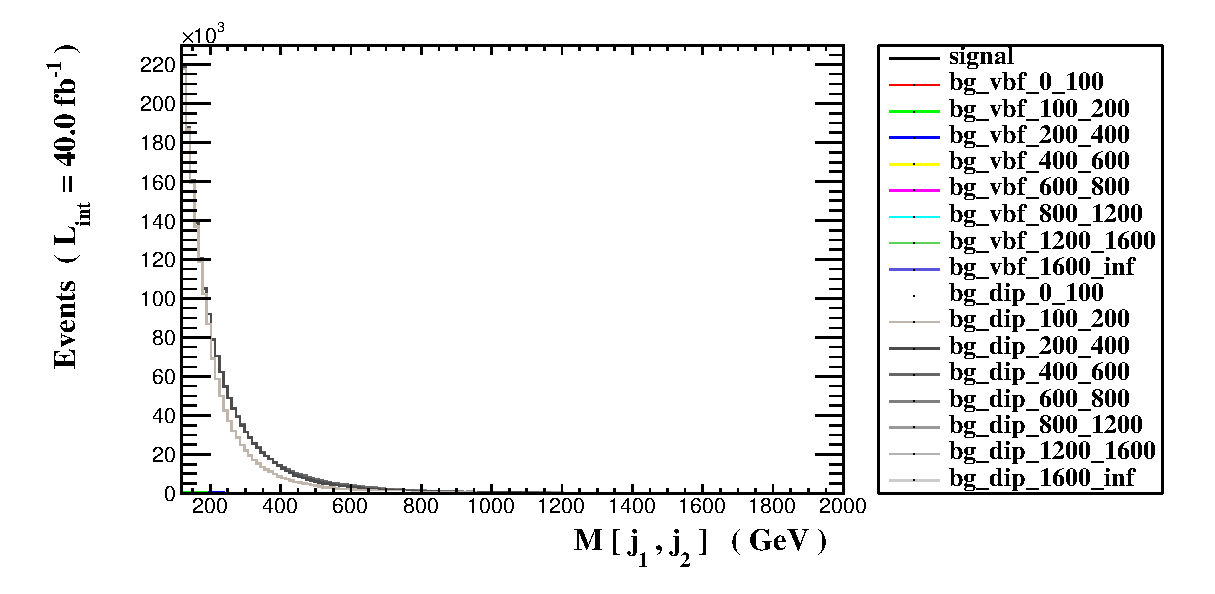
\includegraphics[scale=0.45]{selection_7.eps}\\
\caption{   }
  \end{center}
\end{figure}
      \newpage
\subsection{ Histogram 9}

\textbf{* Plot: MET}\\
   \begin{table}[H]
  \begin{center}
    \begin{tabular}{|m{23.0mm}|m{23.0mm}|m{18.0mm}|m{19.0mm}|m{19.0mm}|m{19.0mm}|m{19.0mm}|}
      \hline
      {\cellcolor{yellow}         Dataset}& {\cellcolor{yellow}         Integral}& {\cellcolor{yellow}         Entries per event}& {\cellcolor{yellow}         Mean}& {\cellcolor{yellow}         RMS}& {\cellcolor{yellow}         \% underflow}& {\cellcolor{yellow}         \% overflow}\\
      \hline
      {\cellcolor{white}         signal}& {\cellcolor{white}         853}& {\cellcolor{white}         1.0}& {\cellcolor{white}         9.37816e-09}& {\cellcolor{white}         1.182e-08}& {\cellcolor{green}         0.0}& {\cellcolor{green}         0.0}\\
      \hline
      {\cellcolor{white}         bg\_vbf\_0\_100}& {\cellcolor{white}         102}& {\cellcolor{white}         1.0}& {\cellcolor{white}         6.19944e-10}& {\cellcolor{white}         4.643e-10}& {\cellcolor{green}         0.0}& {\cellcolor{green}         0.0}\\
      \hline
      {\cellcolor{white}         bg\_vbf\_100\_200}& {\cellcolor{white}         477}& {\cellcolor{white}         1.0}& {\cellcolor{white}         1.03193e-09}& {\cellcolor{white}         1.184e-09}& {\cellcolor{green}         0.0}& {\cellcolor{green}         0.0}\\
      \hline
      {\cellcolor{white}         bg\_vbf\_200\_400}& {\cellcolor{white}         573}& {\cellcolor{white}         1.0}& {\cellcolor{white}         3.36658e-09}& {\cellcolor{white}         2.26e-09}& {\cellcolor{green}         0.0}& {\cellcolor{green}         0.0}\\
      \hline
      {\cellcolor{white}         bg\_vbf\_400\_600}& {\cellcolor{white}         174}& {\cellcolor{white}         1.0}& {\cellcolor{white}         4.57571e-09}& {\cellcolor{white}         2.628e-09}& {\cellcolor{green}         0.0}& {\cellcolor{green}         0.0}\\
      \hline
      {\cellcolor{white}         bg\_vbf\_600\_800}& {\cellcolor{white}         55.7}& {\cellcolor{white}         1.0}& {\cellcolor{white}         4.94087e-09}& {\cellcolor{white}         2.743e-09}& {\cellcolor{green}         0.0}& {\cellcolor{green}         0.0}\\
      \hline
      {\cellcolor{white}         bg\_vbf\_800\_1200}& {\cellcolor{white}         20.2}& {\cellcolor{white}         1.0}& {\cellcolor{white}         5.22726e-09}& {\cellcolor{white}         3.088e-09}& {\cellcolor{green}         0.0}& {\cellcolor{green}         0.0}\\
      \hline
      {\cellcolor{white}         bg\_vbf\_1200\_1600}& {\cellcolor{white}         2.25}& {\cellcolor{white}         1.0}& {\cellcolor{white}         6.30339e-09}& {\cellcolor{white}         6.791e-09}& {\cellcolor{green}         0.0}& {\cellcolor{green}         0.0}\\
      \hline
      {\cellcolor{white}         bg\_vbf\_1600\_inf}& {\cellcolor{white}         0.403}& {\cellcolor{white}         1.0}& {\cellcolor{white}         1.03516e-08}& {\cellcolor{white}         1.322e-08}& {\cellcolor{green}         0.0}& {\cellcolor{green}         0.0}\\
      \hline
      {\cellcolor{white}         bg\_dip\_0\_100}& {\cellcolor{white}         117}& {\cellcolor{white}         1.0}& {\cellcolor{white}         7.65424e-10}& {\cellcolor{white}         5.853e-10}& {\cellcolor{green}         0.0}& {\cellcolor{green}         0.0}\\
      \hline
      {\cellcolor{white}         bg\_dip\_100\_200}& {\cellcolor{white}         496}& {\cellcolor{white}         1.0}& {\cellcolor{white}         1.18704e-09}& {\cellcolor{white}         1.387e-09}& {\cellcolor{green}         0.0}& {\cellcolor{green}         0.0}\\
      \hline
      {\cellcolor{white}         bg\_dip\_200\_400}& {\cellcolor{white}         814}& {\cellcolor{white}         1.0}& {\cellcolor{white}         3.50088e-09}& {\cellcolor{white}         2.275e-09}& {\cellcolor{green}         0.0}& {\cellcolor{green}         0.0}\\
      \hline
      {\cellcolor{white}         bg\_dip\_400\_600}& {\cellcolor{white}         531}& {\cellcolor{white}         1.0}& {\cellcolor{white}         4.48695e-09}& {\cellcolor{white}         2.593e-09}& {\cellcolor{green}         0.0}& {\cellcolor{green}         0.0}\\
      \hline
      {\cellcolor{white}         bg\_dip\_600\_800}& {\cellcolor{white}         263}& {\cellcolor{white}         1.0}& {\cellcolor{white}         4.80027e-09}& {\cellcolor{white}         2.685e-09}& {\cellcolor{green}         0.0}& {\cellcolor{green}         0.0}\\
      \hline
      {\cellcolor{white}         bg\_dip\_800\_1200}& {\cellcolor{white}         96.6}& {\cellcolor{white}         1.0}& {\cellcolor{white}         5.05807e-09}& {\cellcolor{white}         2.996e-09}& {\cellcolor{green}         0.0}& {\cellcolor{green}         0.0}\\
      \hline
      {\cellcolor{white}         bg\_dip\_1200\_1600}& {\cellcolor{white}         10.8}& {\cellcolor{white}         1.0}& {\cellcolor{white}         5.73972e-09}& {\cellcolor{white}         5.438e-09}& {\cellcolor{green}         0.0}& {\cellcolor{green}         0.0}\\
      \hline
      {\cellcolor{white}         bg\_dip\_1600\_inf}& {\cellcolor{white}         2.03}& {\cellcolor{white}         1.0}& {\cellcolor{white}         9.32802e-09}& {\cellcolor{white}         1.244e-08}& {\cellcolor{green}         0.0}& {\cellcolor{green}         0.0}\\
\hline
    \end{tabular}
  \end{center}
\end{table}

\begin{figure}[H]
  \begin{center}
    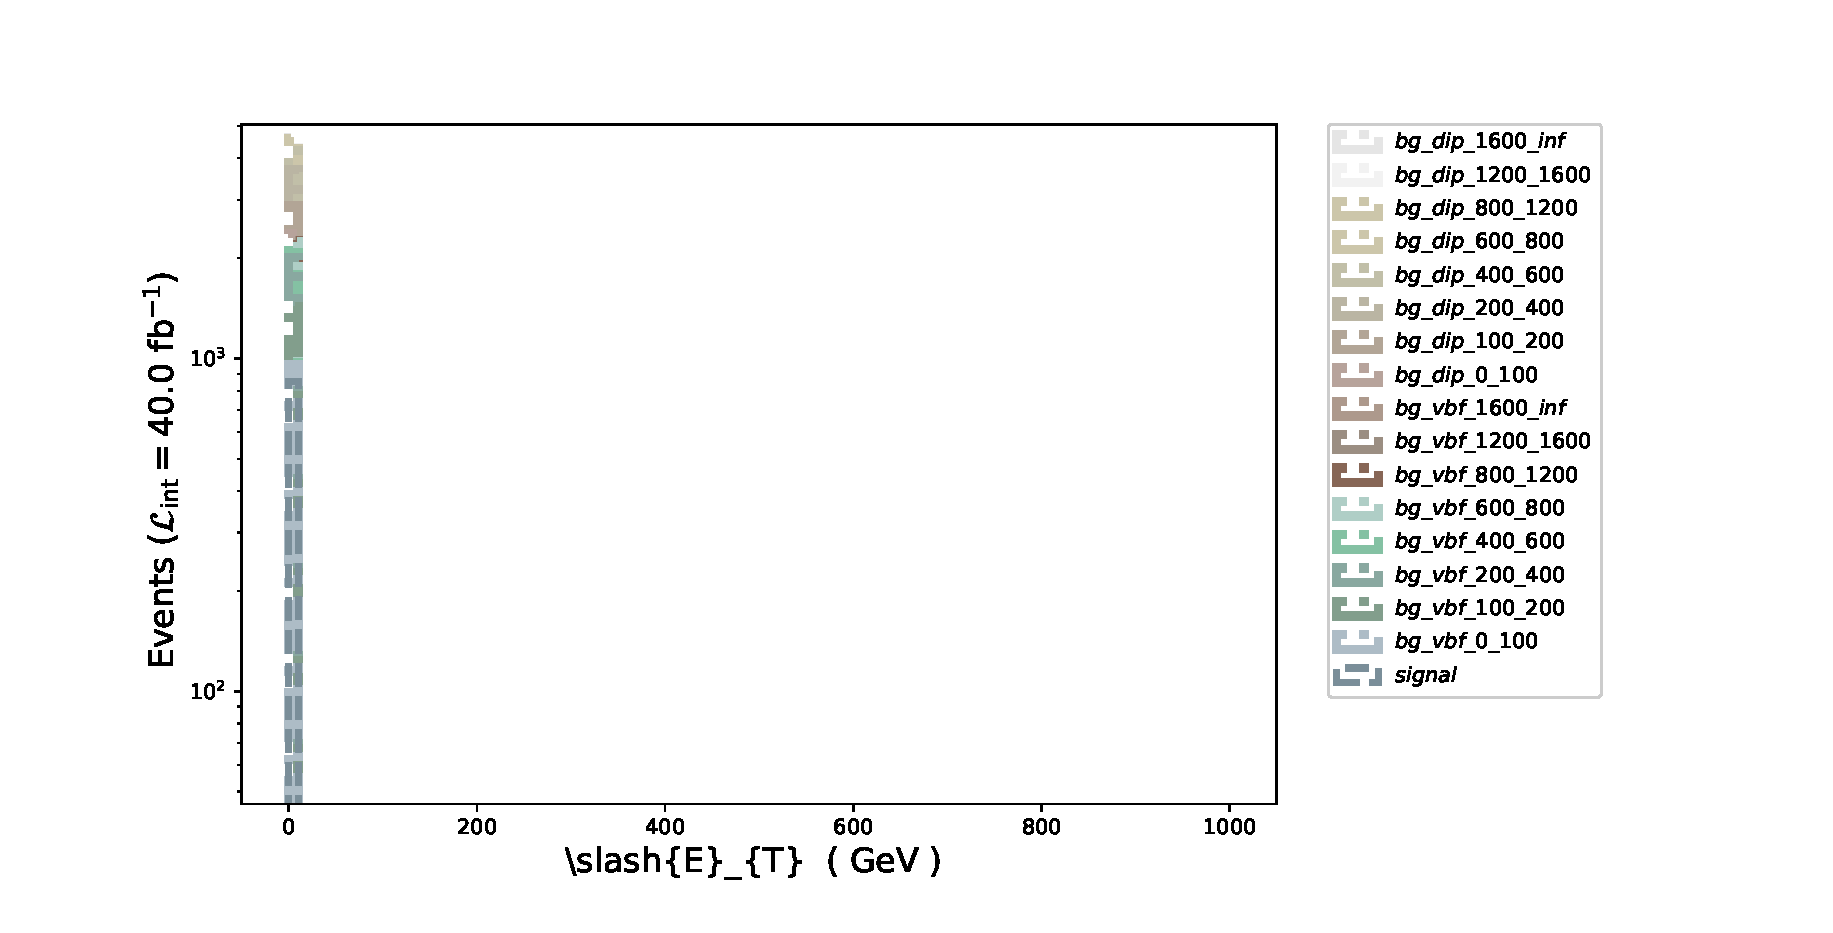
\includegraphics[scale=0.45]{selection_8.eps}\\
\caption{   }
  \end{center}
\end{figure}
      \newpage
\subsection{ Histogram 10}

\textbf{* Plot: sdETA ( jets[1] jets[2] ) }\\
   \begin{table}[H]
  \begin{center}
    \begin{tabular}{|m{23.0mm}|m{23.0mm}|m{18.0mm}|m{19.0mm}|m{19.0mm}|m{19.0mm}|m{19.0mm}|}
      \hline
      {\cellcolor{yellow}         Dataset}& {\cellcolor{yellow}         Integral}& {\cellcolor{yellow}         Entries per event}& {\cellcolor{yellow}         Mean}& {\cellcolor{yellow}         RMS}& {\cellcolor{yellow}         \% underflow}& {\cellcolor{yellow}         \% overflow}\\
      \hline
      {\cellcolor{white}         signal}& {\cellcolor{white}         853}& {\cellcolor{white}         1.0}& {\cellcolor{white}         3.93718}& {\cellcolor{white}         1.261}& {\cellcolor{green}         0.0}& {\cellcolor{green}         0.9681}\\
      \hline
      {\cellcolor{white}         bg\_vbf\_0\_100}& {\cellcolor{white}         102}& {\cellcolor{white}         1.0}& {\cellcolor{white}         7.57435}& {\cellcolor{white}         0.6115}& {\cellcolor{red}         0.0}& {\cellcolor{red}         23.21}\\
      \hline
      {\cellcolor{white}         bg\_vbf\_100\_200}& {\cellcolor{white}         477}& {\cellcolor{white}         1.0}& {\cellcolor{white}         6.40026}& {\cellcolor{white}         0.6673}& {\cellcolor{green}         0.0}& {\cellcolor{green}         2.156}\\
      \hline
      {\cellcolor{white}         bg\_vbf\_200\_400}& {\cellcolor{white}         573}& {\cellcolor{white}         1.0}& {\cellcolor{white}         5.25178}& {\cellcolor{white}         0.7177}& {\cellcolor{green}         0.0}& {\cellcolor{green}         0.03453}\\
      \hline
      {\cellcolor{white}         bg\_vbf\_400\_600}& {\cellcolor{white}         174}& {\cellcolor{white}         1.0}& {\cellcolor{white}         4.1828}& {\cellcolor{white}         0.7028}& {\cellcolor{green}         0.0}& {\cellcolor{green}         0.0}\\
      \hline
      {\cellcolor{white}         bg\_vbf\_600\_800}& {\cellcolor{white}         55.7}& {\cellcolor{white}         1.0}& {\cellcolor{white}         3.57723}& {\cellcolor{white}         0.6768}& {\cellcolor{green}         0.0}& {\cellcolor{green}         0.0}\\
      \hline
      {\cellcolor{white}         bg\_vbf\_800\_1200}& {\cellcolor{white}         20.2}& {\cellcolor{white}         1.0}& {\cellcolor{white}         3.35934}& {\cellcolor{white}         0.5677}& {\cellcolor{green}         0.0}& {\cellcolor{green}         0.0}\\
      \hline
      {\cellcolor{white}         bg\_vbf\_1200\_1600}& {\cellcolor{white}         2.25}& {\cellcolor{white}         1.0}& {\cellcolor{white}         3.14504}& {\cellcolor{white}         0.4308}& {\cellcolor{green}         0.0}& {\cellcolor{green}         0.0}\\
      \hline
      {\cellcolor{white}         bg\_vbf\_1600\_inf}& {\cellcolor{white}         0.403}& {\cellcolor{white}         1.0}& {\cellcolor{white}         3.00196}& {\cellcolor{white}         0.3367}& {\cellcolor{green}         0.0}& {\cellcolor{green}         0.0}\\
      \hline
      {\cellcolor{white}         bg\_dip\_0\_100}& {\cellcolor{white}         117}& {\cellcolor{white}         1.0}& {\cellcolor{white}         7.31275}& {\cellcolor{white}         0.3459}& {\cellcolor{green}         0.0}& {\cellcolor{green}         4.448}\\
      \hline
      {\cellcolor{white}         bg\_dip\_100\_200}& {\cellcolor{white}         496}& {\cellcolor{white}         1.0}& {\cellcolor{white}         6.11125}& {\cellcolor{white}         0.5289}& {\cellcolor{green}         0.0}& {\cellcolor{green}         0.0}\\
      \hline
      {\cellcolor{white}         bg\_dip\_200\_400}& {\cellcolor{white}         814}& {\cellcolor{white}         1.0}& {\cellcolor{white}         4.81866}& {\cellcolor{white}         0.5746}& {\cellcolor{green}         0.0}& {\cellcolor{green}         0.0}\\
      \hline
      {\cellcolor{white}         bg\_dip\_400\_600}& {\cellcolor{white}         531}& {\cellcolor{white}         1.0}& {\cellcolor{white}         3.73343}& {\cellcolor{white}         0.5229}& {\cellcolor{green}         0.0}& {\cellcolor{green}         0.0}\\
      \hline
      {\cellcolor{white}         bg\_dip\_600\_800}& {\cellcolor{white}         263}& {\cellcolor{white}         1.0}& {\cellcolor{white}         3.17164}& {\cellcolor{white}         0.476}& {\cellcolor{green}         0.0}& {\cellcolor{green}         0.0}\\
      \hline
      {\cellcolor{white}         bg\_dip\_800\_1200}& {\cellcolor{white}         96.6}& {\cellcolor{white}         1.0}& {\cellcolor{white}         3.0772}& {\cellcolor{white}         0.4164}& {\cellcolor{green}         0.0}& {\cellcolor{green}         0.0}\\
      \hline
      {\cellcolor{white}         bg\_dip\_1200\_1600}& {\cellcolor{white}         10.8}& {\cellcolor{white}         1.0}& {\cellcolor{white}         2.98817}& {\cellcolor{white}         0.3412}& {\cellcolor{green}         0.0}& {\cellcolor{green}         0.0}\\
      \hline
      {\cellcolor{white}         bg\_dip\_1600\_inf}& {\cellcolor{white}         2.03}& {\cellcolor{white}         1.0}& {\cellcolor{white}         2.90097}& {\cellcolor{white}         0.2648}& {\cellcolor{green}         0.0}& {\cellcolor{green}         0.0}\\
\hline
    \end{tabular}
  \end{center}
\end{table}

\begin{figure}[H]
  \begin{center}
    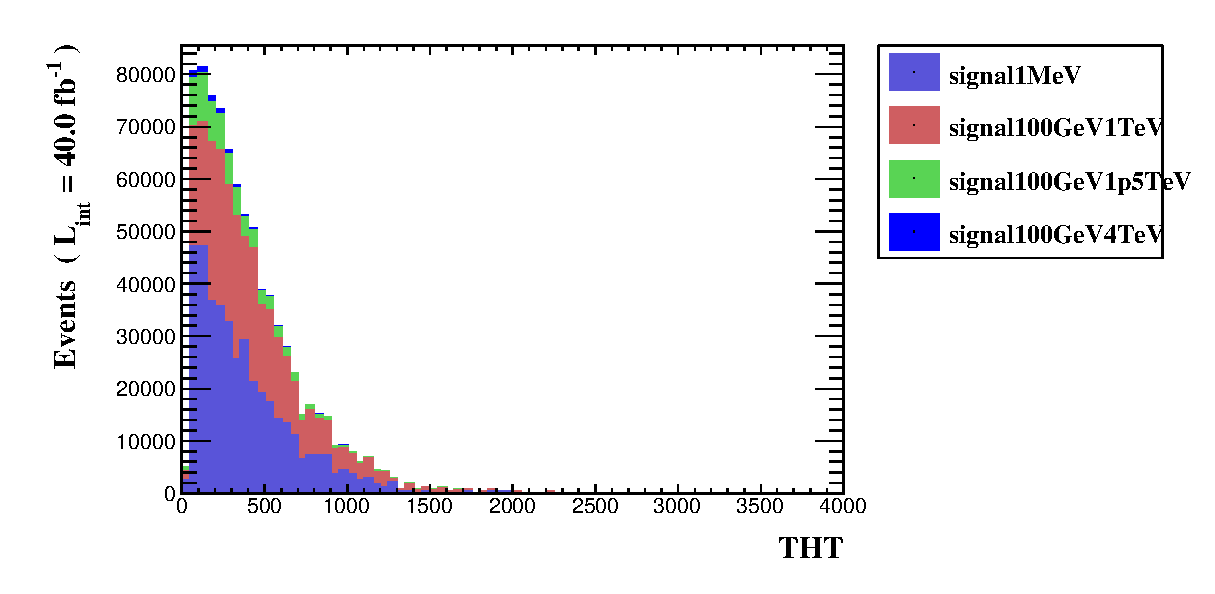
\includegraphics[scale=0.45]{selection_9.eps}\\
\caption{   }
  \end{center}
\end{figure}
      \newpage
\subsection{ Histogram 11}

\textbf{* Plot: M ( a[1] a[2] ) }\\
   \begin{table}[H]
  \begin{center}
    \begin{tabular}{|m{23.0mm}|m{23.0mm}|m{18.0mm}|m{19.0mm}|m{19.0mm}|m{19.0mm}|m{19.0mm}|}
      \hline
      {\cellcolor{yellow}         Dataset}& {\cellcolor{yellow}         Integral}& {\cellcolor{yellow}         Entries per event}& {\cellcolor{yellow}         Mean}& {\cellcolor{yellow}         RMS}& {\cellcolor{yellow}         \% underflow}& {\cellcolor{yellow}         \% overflow}\\
      \hline
      {\cellcolor{white}         signal}& {\cellcolor{white}         853}& {\cellcolor{white}         1.0}& {\cellcolor{white}         996.626}& {\cellcolor{white}         716.7}& {\cellcolor{red}         0.0}& {\cellcolor{red}         39.92}\\
      \hline
      {\cellcolor{white}         bg\_vbf\_0\_100}& {\cellcolor{white}         102}& {\cellcolor{white}         1.0}& {\cellcolor{white}         74.8671}& {\cellcolor{white}         64.42}& {\cellcolor{green}         0.0}& {\cellcolor{green}         0.01176}\\
      \hline
      {\cellcolor{white}         bg\_vbf\_100\_200}& {\cellcolor{white}         477}& {\cellcolor{white}         1.0}& {\cellcolor{white}         89.3839}& {\cellcolor{white}         83.48}& {\cellcolor{green}         0.0}& {\cellcolor{green}         0.0399}\\
      \hline
      {\cellcolor{white}         bg\_vbf\_200\_400}& {\cellcolor{white}         573}& {\cellcolor{white}         1.0}& {\cellcolor{white}         113.725}& {\cellcolor{white}         113.1}& {\cellcolor{green}         0.0}& {\cellcolor{green}         0.1218}\\
      \hline
      {\cellcolor{white}         bg\_vbf\_400\_600}& {\cellcolor{white}         174}& {\cellcolor{white}         1.0}& {\cellcolor{white}         133.277}& {\cellcolor{white}         137.6}& {\cellcolor{green}         0.0}& {\cellcolor{green}         0.2421}\\
      \hline
      {\cellcolor{white}         bg\_vbf\_600\_800}& {\cellcolor{white}         55.7}& {\cellcolor{white}         1.0}& {\cellcolor{white}         145.549}& {\cellcolor{white}         156.9}& {\cellcolor{green}         0.0}& {\cellcolor{green}         0.4347}\\
      \hline
      {\cellcolor{white}         bg\_vbf\_800\_1200}& {\cellcolor{white}         20.2}& {\cellcolor{white}         1.0}& {\cellcolor{white}         163.011}& {\cellcolor{white}         179.6}& {\cellcolor{green}         0.0}& {\cellcolor{green}         0.7012}\\
      \hline
      {\cellcolor{white}         bg\_vbf\_1200\_1600}& {\cellcolor{white}         2.25}& {\cellcolor{white}         1.0}& {\cellcolor{white}         176.229}& {\cellcolor{white}         203.3}& {\cellcolor{green}         0.0}& {\cellcolor{green}         1.067}\\
      \hline
      {\cellcolor{white}         bg\_vbf\_1600\_inf}& {\cellcolor{white}         0.403}& {\cellcolor{white}         1.0}& {\cellcolor{white}         180.895}& {\cellcolor{white}         212.8}& {\cellcolor{green}         0.0}& {\cellcolor{green}         1.247}\\
      \hline
      {\cellcolor{white}         bg\_dip\_0\_100}& {\cellcolor{white}         117}& {\cellcolor{white}         1.0}& {\cellcolor{white}         67.9791}& {\cellcolor{white}         48.97}& {\cellcolor{green}         0.0}& {\cellcolor{green}         0.0}\\
      \hline
      {\cellcolor{white}         bg\_dip\_100\_200}& {\cellcolor{white}         496}& {\cellcolor{white}         1.0}& {\cellcolor{white}         81.4606}& {\cellcolor{white}         86.76}& {\cellcolor{green}         0.0}& {\cellcolor{green}         0.0}\\
      \hline
      {\cellcolor{white}         bg\_dip\_200\_400}& {\cellcolor{white}         814}& {\cellcolor{white}         1.0}& {\cellcolor{white}         101.829}& {\cellcolor{white}         117.4}& {\cellcolor{green}         0.0}& {\cellcolor{green}         0.08477}\\
      \hline
      {\cellcolor{white}         bg\_dip\_400\_600}& {\cellcolor{white}         531}& {\cellcolor{white}         1.0}& {\cellcolor{white}         116.247}& {\cellcolor{white}         141.0}& {\cellcolor{green}         0.0}& {\cellcolor{green}         0.2657}\\
      \hline
      {\cellcolor{white}         bg\_dip\_600\_800}& {\cellcolor{white}         263}& {\cellcolor{white}         1.0}& {\cellcolor{white}         127.197}& {\cellcolor{white}         151.3}& {\cellcolor{green}         0.0}& {\cellcolor{green}         0.3668}\\
      \hline
      {\cellcolor{white}         bg\_dip\_800\_1200}& {\cellcolor{white}         96.6}& {\cellcolor{white}         1.0}& {\cellcolor{white}         148.707}& {\cellcolor{white}         182.6}& {\cellcolor{green}         0.0}& {\cellcolor{green}         0.6794}\\
      \hline
      {\cellcolor{white}         bg\_dip\_1200\_1600}& {\cellcolor{white}         10.8}& {\cellcolor{white}         1.0}& {\cellcolor{white}         165.538}& {\cellcolor{white}         206.2}& {\cellcolor{green}         0.0}& {\cellcolor{green}         1.101}\\
      \hline
      {\cellcolor{white}         bg\_dip\_1600\_inf}& {\cellcolor{white}         2.03}& {\cellcolor{white}         1.0}& {\cellcolor{white}         178.029}& {\cellcolor{white}         215.3}& {\cellcolor{green}         0.0}& {\cellcolor{green}         1.193}\\
\hline
    \end{tabular}
  \end{center}
\end{table}

\begin{figure}[H]
  \begin{center}
    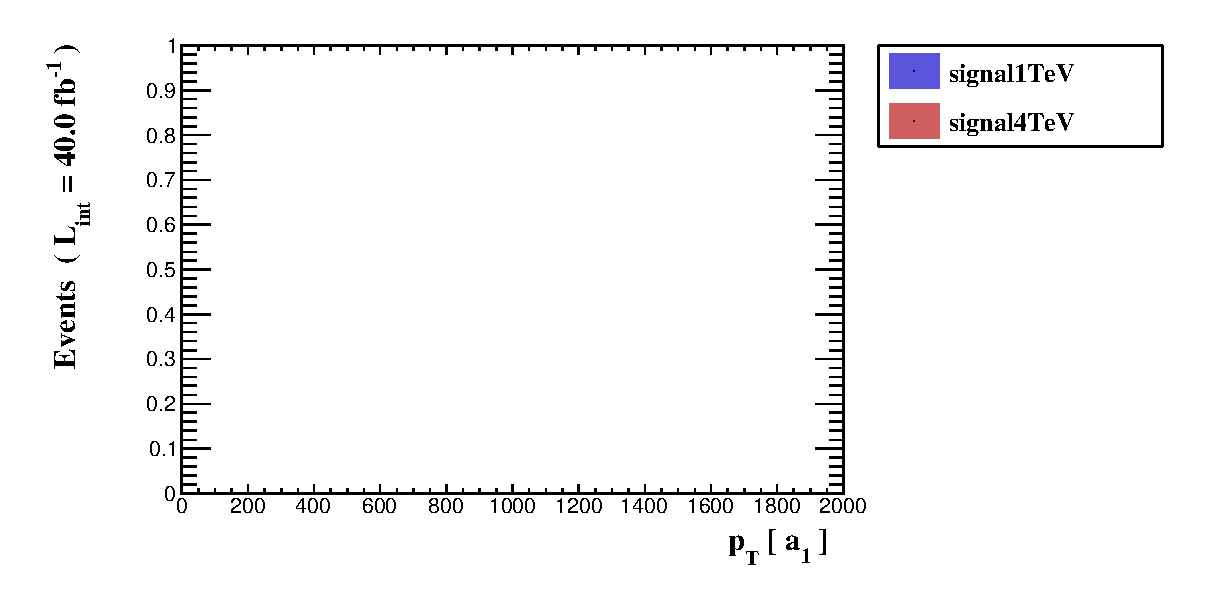
\includegraphics[scale=0.45]{selection_10.eps}\\
\caption{   }
  \end{center}
\end{figure}
      \newpage
\subsection{ Histogram 12}

\textbf{* Plot: PT ( a[1] ) }\\
   \begin{table}[H]
  \begin{center}
    \begin{tabular}{|m{23.0mm}|m{23.0mm}|m{18.0mm}|m{19.0mm}|m{19.0mm}|m{19.0mm}|m{19.0mm}|}
      \hline
      {\cellcolor{yellow}         Dataset}& {\cellcolor{yellow}         Integral}& {\cellcolor{yellow}         Entries per event}& {\cellcolor{yellow}         Mean}& {\cellcolor{yellow}         RMS}& {\cellcolor{yellow}         \% underflow}& {\cellcolor{yellow}         \% overflow}\\
      \hline
      {\cellcolor{white}         signal}& {\cellcolor{white}         853}& {\cellcolor{white}         1.0}& {\cellcolor{white}         656.187}& {\cellcolor{white}         372.1}& {\cellcolor{red}         0.0}& {\cellcolor{red}         16.29}\\
      \hline
      {\cellcolor{white}         bg\_vbf\_0\_100}& {\cellcolor{white}         102}& {\cellcolor{white}         1.0}& {\cellcolor{white}         37.6561}& {\cellcolor{white}         21.46}& {\cellcolor{green}         0.0}& {\cellcolor{green}         0.0}\\
      \hline
      {\cellcolor{white}         bg\_vbf\_100\_200}& {\cellcolor{white}         477}& {\cellcolor{white}         1.0}& {\cellcolor{white}         51.7205}& {\cellcolor{white}         34.53}& {\cellcolor{green}         0.0}& {\cellcolor{green}         0.0}\\
      \hline
      {\cellcolor{white}         bg\_vbf\_200\_400}& {\cellcolor{white}         573}& {\cellcolor{white}         1.0}& {\cellcolor{white}         79.4071}& {\cellcolor{white}         64.6}& {\cellcolor{green}         0.0}& {\cellcolor{green}         0.0}\\
      \hline
      {\cellcolor{white}         bg\_vbf\_400\_600}& {\cellcolor{white}         174}& {\cellcolor{white}         1.0}& {\cellcolor{white}         114.223}& {\cellcolor{white}         106.2}& {\cellcolor{green}         0.0}& {\cellcolor{green}         0.002262}\\
      \hline
      {\cellcolor{white}         bg\_vbf\_600\_800}& {\cellcolor{white}         55.7}& {\cellcolor{white}         1.0}& {\cellcolor{white}         140.703}& {\cellcolor{white}         144.4}& {\cellcolor{green}         0.0}& {\cellcolor{green}         0.009507}\\
      \hline
      {\cellcolor{white}         bg\_vbf\_800\_1200}& {\cellcolor{white}         20.2}& {\cellcolor{white}         1.0}& {\cellcolor{white}         176.007}& {\cellcolor{white}         200.4}& {\cellcolor{green}         0.0}& {\cellcolor{green}         0.4498}\\
      \hline
      {\cellcolor{white}         bg\_vbf\_1200\_1600}& {\cellcolor{white}         2.25}& {\cellcolor{white}         1.0}& {\cellcolor{white}         209.34}& {\cellcolor{white}         270.7}& {\cellcolor{green}         0.0}& {\cellcolor{green}         3.606}\\
      \hline
      {\cellcolor{white}         bg\_vbf\_1600\_inf}& {\cellcolor{white}         0.403}& {\cellcolor{white}         1.0}& {\cellcolor{white}         224.24}& {\cellcolor{white}         328.6}& {\cellcolor{green}         0.0}& {\cellcolor{green}         4.472}\\
      \hline
      {\cellcolor{white}         bg\_dip\_0\_100}& {\cellcolor{white}         117}& {\cellcolor{white}         1.0}& {\cellcolor{white}         39.6474}& {\cellcolor{white}         25.66}& {\cellcolor{green}         0.0}& {\cellcolor{green}         0.0}\\
      \hline
      {\cellcolor{white}         bg\_dip\_100\_200}& {\cellcolor{white}         496}& {\cellcolor{white}         1.0}& {\cellcolor{white}         55.7039}& {\cellcolor{white}         43.6}& {\cellcolor{green}         0.0}& {\cellcolor{green}         0.0}\\
      \hline
      {\cellcolor{white}         bg\_dip\_200\_400}& {\cellcolor{white}         814}& {\cellcolor{white}         1.0}& {\cellcolor{white}         77.1175}& {\cellcolor{white}         73.41}& {\cellcolor{green}         0.0}& {\cellcolor{green}         0.0}\\
      \hline
      {\cellcolor{white}         bg\_dip\_400\_600}& {\cellcolor{white}         531}& {\cellcolor{white}         1.0}& {\cellcolor{white}         89.1572}& {\cellcolor{white}         97.37}& {\cellcolor{green}         0.0}& {\cellcolor{green}         0.0}\\
      \hline
      {\cellcolor{white}         bg\_dip\_600\_800}& {\cellcolor{white}         263}& {\cellcolor{white}         1.0}& {\cellcolor{white}         102.356}& {\cellcolor{white}         117.0}& {\cellcolor{green}         0.0}& {\cellcolor{green}         0.007647}\\
      \hline
      {\cellcolor{white}         bg\_dip\_800\_1200}& {\cellcolor{white}         96.6}& {\cellcolor{white}         1.0}& {\cellcolor{white}         129.437}& {\cellcolor{white}         168.5}& {\cellcolor{green}         0.0}& {\cellcolor{green}         0.3952}\\
      \hline
      {\cellcolor{white}         bg\_dip\_1200\_1600}& {\cellcolor{white}         10.8}& {\cellcolor{white}         1.0}& {\cellcolor{white}         147.694}& {\cellcolor{white}         223.8}& {\cellcolor{green}         0.0}& {\cellcolor{green}         2.441}\\
      \hline
      {\cellcolor{white}         bg\_dip\_1600\_inf}& {\cellcolor{white}         2.03}& {\cellcolor{white}         1.0}& {\cellcolor{white}         147.279}& {\cellcolor{white}         239.6}& {\cellcolor{green}         0.0}& {\cellcolor{green}         1.798}\\
\hline
    \end{tabular}
  \end{center}
\end{table}

\begin{figure}[H]
  \begin{center}
    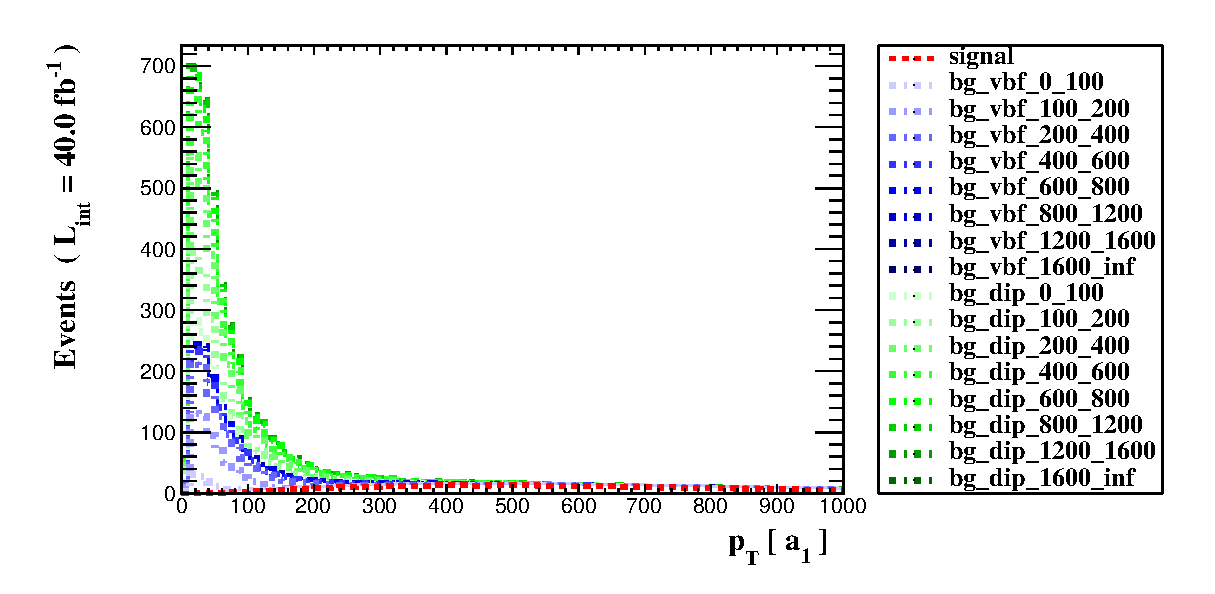
\includegraphics[scale=0.45]{selection_11.eps}\\
\caption{   }
  \end{center}
\end{figure}
      \newpage
\subsection{ Histogram 13}

\textbf{* Plot: PT ( a[2] ) }\\
   \begin{table}[H]
  \begin{center}
    \begin{tabular}{|m{23.0mm}|m{23.0mm}|m{18.0mm}|m{19.0mm}|m{19.0mm}|m{19.0mm}|m{19.0mm}|}
      \hline
      {\cellcolor{yellow}         Dataset}& {\cellcolor{yellow}         Integral}& {\cellcolor{yellow}         Entries per event}& {\cellcolor{yellow}         Mean}& {\cellcolor{yellow}         RMS}& {\cellcolor{yellow}         \% underflow}& {\cellcolor{yellow}         \% overflow}\\
      \hline
      {\cellcolor{white}         signal}& {\cellcolor{white}         853}& {\cellcolor{white}         1.0}& {\cellcolor{white}         352.1}& {\cellcolor{white}         284.5}& {\cellcolor{green}         0.0}& {\cellcolor{green}         3.577}\\
      \hline
      {\cellcolor{white}         bg\_vbf\_0\_100}& {\cellcolor{white}         102}& {\cellcolor{white}         1.0}& {\cellcolor{white}         19.9879}& {\cellcolor{white}         13.16}& {\cellcolor{green}         0.0}& {\cellcolor{green}         0.0}\\
      \hline
      {\cellcolor{white}         bg\_vbf\_100\_200}& {\cellcolor{white}         477}& {\cellcolor{white}         1.0}& {\cellcolor{white}         23.3502}& {\cellcolor{white}         18.44}& {\cellcolor{green}         0.0}& {\cellcolor{green}         0.0}\\
      \hline
      {\cellcolor{white}         bg\_vbf\_200\_400}& {\cellcolor{white}         573}& {\cellcolor{white}         1.0}& {\cellcolor{white}         28.1052}& {\cellcolor{white}         26.02}& {\cellcolor{green}         0.0}& {\cellcolor{green}         0.0}\\
      \hline
      {\cellcolor{white}         bg\_vbf\_400\_600}& {\cellcolor{white}         174}& {\cellcolor{white}         1.0}& {\cellcolor{white}         33.0218}& {\cellcolor{white}         34.3}& {\cellcolor{green}         0.0}& {\cellcolor{green}         0.0}\\
      \hline
      {\cellcolor{white}         bg\_vbf\_600\_800}& {\cellcolor{white}         55.7}& {\cellcolor{white}         1.0}& {\cellcolor{white}         36.2955}& {\cellcolor{white}         40.84}& {\cellcolor{green}         0.0}& {\cellcolor{green}         0.0004532}\\
      \hline
      {\cellcolor{white}         bg\_vbf\_800\_1200}& {\cellcolor{white}         20.2}& {\cellcolor{white}         1.0}& {\cellcolor{white}         39.6378}& {\cellcolor{white}         47.89}& {\cellcolor{green}         0.0}& {\cellcolor{green}         0.0}\\
      \hline
      {\cellcolor{white}         bg\_vbf\_1200\_1600}& {\cellcolor{white}         2.25}& {\cellcolor{white}         1.0}& {\cellcolor{white}         42.8767}& {\cellcolor{white}         56.71}& {\cellcolor{green}         0.0}& {\cellcolor{green}         0.005763}\\
      \hline
      {\cellcolor{white}         bg\_vbf\_1600\_inf}& {\cellcolor{white}         0.403}& {\cellcolor{white}         1.0}& {\cellcolor{white}         43.8682}& {\cellcolor{white}         60.26}& {\cellcolor{green}         0.0}& {\cellcolor{green}         0.01411}\\
      \hline
      {\cellcolor{white}         bg\_dip\_0\_100}& {\cellcolor{white}         117}& {\cellcolor{white}         1.0}& {\cellcolor{white}         21.3156}& {\cellcolor{white}         12.28}& {\cellcolor{green}         0.0}& {\cellcolor{green}         0.0}\\
      \hline
      {\cellcolor{white}         bg\_dip\_100\_200}& {\cellcolor{white}         496}& {\cellcolor{white}         1.0}& {\cellcolor{white}         21.5768}& {\cellcolor{white}         16.61}& {\cellcolor{green}         0.0}& {\cellcolor{green}         0.0}\\
      \hline
      {\cellcolor{white}         bg\_dip\_200\_400}& {\cellcolor{white}         814}& {\cellcolor{white}         1.0}& {\cellcolor{white}         24.8054}& {\cellcolor{white}         22.89}& {\cellcolor{green}         0.0}& {\cellcolor{green}         0.0}\\
      \hline
      {\cellcolor{white}         bg\_dip\_400\_600}& {\cellcolor{white}         531}& {\cellcolor{white}         1.0}& {\cellcolor{white}         26.8814}& {\cellcolor{white}         26.02}& {\cellcolor{green}         0.0}& {\cellcolor{green}         0.0}\\
      \hline
      {\cellcolor{white}         bg\_dip\_600\_800}& {\cellcolor{white}         263}& {\cellcolor{white}         1.0}& {\cellcolor{white}         28.87}& {\cellcolor{white}         29.88}& {\cellcolor{green}         0.0}& {\cellcolor{green}         0.0}\\
      \hline
      {\cellcolor{white}         bg\_dip\_800\_1200}& {\cellcolor{white}         96.6}& {\cellcolor{white}         1.0}& {\cellcolor{white}         31.6547}& {\cellcolor{white}         35.19}& {\cellcolor{green}         0.0}& {\cellcolor{green}         0.0}\\
      \hline
      {\cellcolor{white}         bg\_dip\_1200\_1600}& {\cellcolor{white}         10.8}& {\cellcolor{white}         1.0}& {\cellcolor{white}         33.502}& {\cellcolor{white}         38.62}& {\cellcolor{green}         0.0}& {\cellcolor{green}         0.0}\\
      \hline
      {\cellcolor{white}         bg\_dip\_1600\_inf}& {\cellcolor{white}         2.03}& {\cellcolor{white}         1.0}& {\cellcolor{white}         34.6417}& {\cellcolor{white}         42.68}& {\cellcolor{green}         0.0}& {\cellcolor{green}         0.00892}\\
\hline
    \end{tabular}
  \end{center}
\end{table}

\begin{figure}[H]
  \begin{center}
    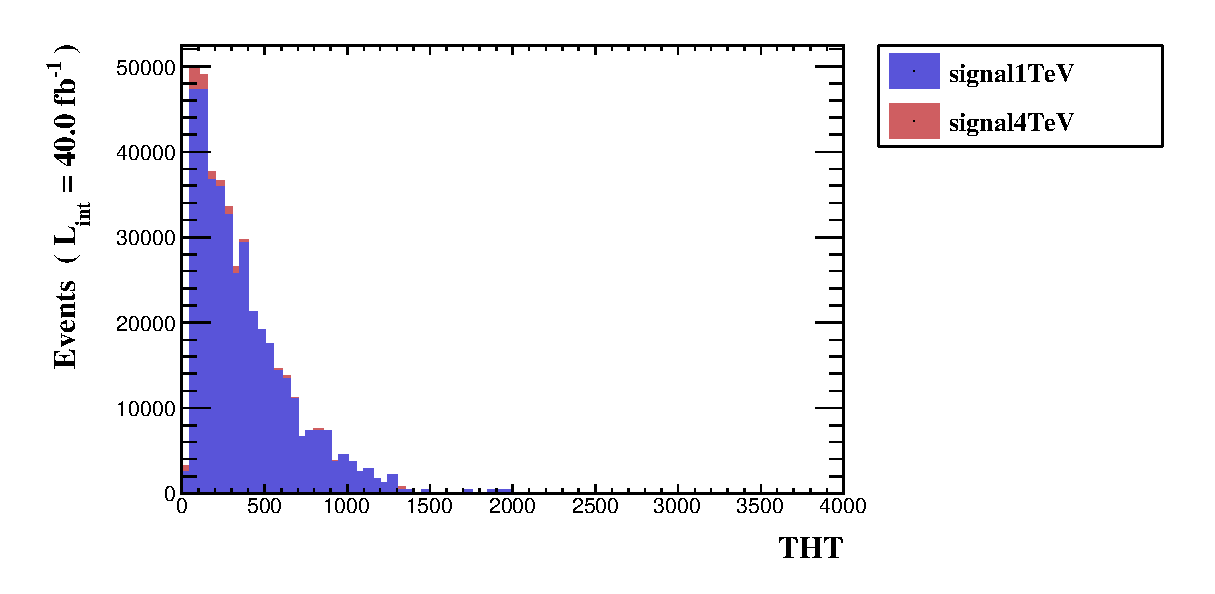
\includegraphics[scale=0.45]{selection_12.eps}\\
\caption{   }
  \end{center}
\end{figure}
      \newpage
\subsection{ Histogram 14}

\textbf{* Plot: THT}\\
   \begin{table}[H]
  \begin{center}
    \begin{tabular}{|m{23.0mm}|m{23.0mm}|m{18.0mm}|m{19.0mm}|m{19.0mm}|m{19.0mm}|m{19.0mm}|}
      \hline
      {\cellcolor{yellow}         Dataset}& {\cellcolor{yellow}         Integral}& {\cellcolor{yellow}         Entries per event}& {\cellcolor{yellow}         Mean}& {\cellcolor{yellow}         RMS}& {\cellcolor{yellow}         \% underflow}& {\cellcolor{yellow}         \% overflow}\\
      \hline
      {\cellcolor{white}         signal}& {\cellcolor{white}         853}& {\cellcolor{white}         1.0}& {\cellcolor{white}         752.478}& {\cellcolor{white}         393.0}& {\cellcolor{red}         0.0}& {\cellcolor{red}         23.55}\\
      \hline
      {\cellcolor{white}         bg\_vbf\_0\_100}& {\cellcolor{white}         102}& {\cellcolor{white}         1.0}& {\cellcolor{white}         80.0995}& {\cellcolor{white}         13.51}& {\cellcolor{green}         0.0}& {\cellcolor{green}         0.0}\\
      \hline
      {\cellcolor{white}         bg\_vbf\_100\_200}& {\cellcolor{white}         477}& {\cellcolor{white}         1.0}& {\cellcolor{white}         148.512}& {\cellcolor{white}         28.32}& {\cellcolor{green}         0.0}& {\cellcolor{green}         0.0}\\
      \hline
      {\cellcolor{white}         bg\_vbf\_200\_400}& {\cellcolor{white}         573}& {\cellcolor{white}         1.0}& {\cellcolor{white}         280.111}& {\cellcolor{white}         55.42}& {\cellcolor{green}         0.0}& {\cellcolor{green}         0.0}\\
      \hline
      {\cellcolor{white}         bg\_vbf\_400\_600}& {\cellcolor{white}         174}& {\cellcolor{white}         1.0}& {\cellcolor{white}         481.428}& {\cellcolor{white}         56.16}& {\cellcolor{green}         0.0}& {\cellcolor{green}         0.0}\\
      \hline
      {\cellcolor{white}         bg\_vbf\_600\_800}& {\cellcolor{white}         55.7}& {\cellcolor{white}         1.0}& {\cellcolor{white}         678.908}& {\cellcolor{white}         55.16}& {\cellcolor{green}         0.0}& {\cellcolor{green}         0.0}\\
      \hline
      {\cellcolor{white}         bg\_vbf\_800\_1200}& {\cellcolor{white}         20.2}& {\cellcolor{white}         1.0}& {\cellcolor{white}         927.914}& {\cellcolor{white}         102.4}& {\cellcolor{red}         0.0}& {\cellcolor{red}         23.73}\\
      \hline
      {\cellcolor{white}         bg\_vbf\_1200\_1600}& {\cellcolor{white}         2.25}& {\cellcolor{white}         1.0}& {\cellcolor{white}         1336.37}& {\cellcolor{white}         104.5}& {\cellcolor{red}         0.0}& {\cellcolor{red}         100.0}\\
      \hline
      {\cellcolor{white}         bg\_vbf\_1600\_inf}& {\cellcolor{white}         0.403}& {\cellcolor{white}         1.0}& {\cellcolor{white}         1818.94}& {\cellcolor{white}         218.8}& {\cellcolor{red}         0.0}& {\cellcolor{red}         100.0}\\
      \hline
      {\cellcolor{white}         bg\_dip\_0\_100}& {\cellcolor{white}         117}& {\cellcolor{white}         1.0}& {\cellcolor{white}         81.8197}& {\cellcolor{white}         10.1}& {\cellcolor{green}         0.0}& {\cellcolor{green}         0.0}\\
      \hline
      {\cellcolor{white}         bg\_dip\_100\_200}& {\cellcolor{white}         496}& {\cellcolor{white}         1.0}& {\cellcolor{white}         150.725}& {\cellcolor{white}         28.95}& {\cellcolor{green}         0.0}& {\cellcolor{green}         0.0}\\
      \hline
      {\cellcolor{white}         bg\_dip\_200\_400}& {\cellcolor{white}         814}& {\cellcolor{white}         1.0}& {\cellcolor{white}         291.464}& {\cellcolor{white}         57.47}& {\cellcolor{green}         0.0}& {\cellcolor{green}         0.0}\\
      \hline
      {\cellcolor{white}         bg\_dip\_400\_600}& {\cellcolor{white}         531}& {\cellcolor{white}         1.0}& {\cellcolor{white}         492.287}& {\cellcolor{white}         57.74}& {\cellcolor{green}         0.0}& {\cellcolor{green}         0.0}\\
      \hline
      {\cellcolor{white}         bg\_dip\_600\_800}& {\cellcolor{white}         263}& {\cellcolor{white}         1.0}& {\cellcolor{white}         679.466}& {\cellcolor{white}         54.63}& {\cellcolor{green}         0.0}& {\cellcolor{green}         0.0}\\
      \hline
      {\cellcolor{white}         bg\_dip\_800\_1200}& {\cellcolor{white}         96.6}& {\cellcolor{white}         1.0}& {\cellcolor{white}         928.373}& {\cellcolor{white}         102.3}& {\cellcolor{red}         0.0}& {\cellcolor{red}         23.83}\\
      \hline
      {\cellcolor{white}         bg\_dip\_1200\_1600}& {\cellcolor{white}         10.8}& {\cellcolor{white}         1.0}& {\cellcolor{white}         1336.89}& {\cellcolor{white}         103.8}& {\cellcolor{red}         0.0}& {\cellcolor{red}         100.0}\\
      \hline
      {\cellcolor{white}         bg\_dip\_1600\_inf}& {\cellcolor{white}         2.03}& {\cellcolor{white}         1.0}& {\cellcolor{white}         1828.03}& {\cellcolor{white}         226.7}& {\cellcolor{red}         0.0}& {\cellcolor{red}         100.0}\\
\hline
    \end{tabular}
  \end{center}
\end{table}

\begin{figure}[H]
  \begin{center}
    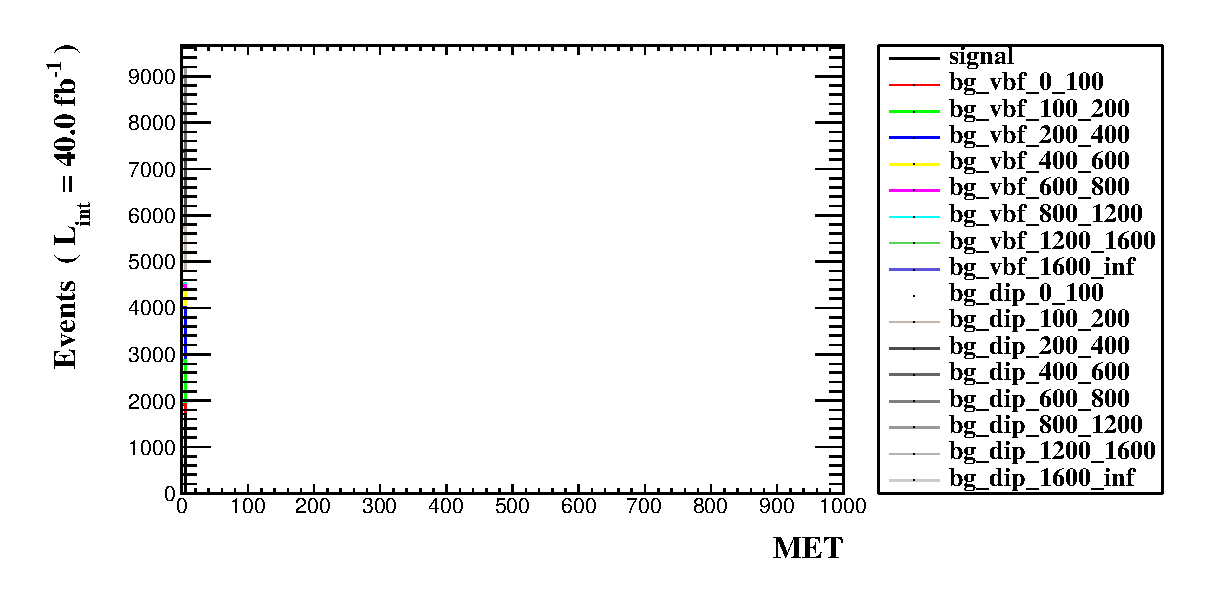
\includegraphics[scale=0.45]{selection_13.eps}\\
\caption{   }
  \end{center}
\end{figure}
      \newpage
\subsection{ Histogram 15}

\textbf{* Plot: MET}\\
   \begin{table}[H]
  \begin{center}
    \begin{tabular}{|m{23.0mm}|m{23.0mm}|m{18.0mm}|m{19.0mm}|m{19.0mm}|m{19.0mm}|m{19.0mm}|}
      \hline
      {\cellcolor{yellow}         Dataset}& {\cellcolor{yellow}         Integral}& {\cellcolor{yellow}         Entries per event}& {\cellcolor{yellow}         Mean}& {\cellcolor{yellow}         RMS}& {\cellcolor{yellow}         \% underflow}& {\cellcolor{yellow}         \% overflow}\\
      \hline
      {\cellcolor{white}         signal}& {\cellcolor{white}         853}& {\cellcolor{white}         1.0}& {\cellcolor{white}         9.37816e-09}& {\cellcolor{white}         1.182e-08}& {\cellcolor{green}         0.0}& {\cellcolor{green}         0.0}\\
      \hline
      {\cellcolor{white}         bg\_vbf\_0\_100}& {\cellcolor{white}         102}& {\cellcolor{white}         1.0}& {\cellcolor{white}         6.19944e-10}& {\cellcolor{white}         4.643e-10}& {\cellcolor{green}         0.0}& {\cellcolor{green}         0.0}\\
      \hline
      {\cellcolor{white}         bg\_vbf\_100\_200}& {\cellcolor{white}         477}& {\cellcolor{white}         1.0}& {\cellcolor{white}         1.03193e-09}& {\cellcolor{white}         1.184e-09}& {\cellcolor{green}         0.0}& {\cellcolor{green}         0.0}\\
      \hline
      {\cellcolor{white}         bg\_vbf\_200\_400}& {\cellcolor{white}         573}& {\cellcolor{white}         1.0}& {\cellcolor{white}         3.36658e-09}& {\cellcolor{white}         2.26e-09}& {\cellcolor{green}         0.0}& {\cellcolor{green}         0.0}\\
      \hline
      {\cellcolor{white}         bg\_vbf\_400\_600}& {\cellcolor{white}         174}& {\cellcolor{white}         1.0}& {\cellcolor{white}         4.57571e-09}& {\cellcolor{white}         2.628e-09}& {\cellcolor{green}         0.0}& {\cellcolor{green}         0.0}\\
      \hline
      {\cellcolor{white}         bg\_vbf\_600\_800}& {\cellcolor{white}         55.7}& {\cellcolor{white}         1.0}& {\cellcolor{white}         4.94087e-09}& {\cellcolor{white}         2.743e-09}& {\cellcolor{green}         0.0}& {\cellcolor{green}         0.0}\\
      \hline
      {\cellcolor{white}         bg\_vbf\_800\_1200}& {\cellcolor{white}         20.2}& {\cellcolor{white}         1.0}& {\cellcolor{white}         5.22726e-09}& {\cellcolor{white}         3.088e-09}& {\cellcolor{green}         0.0}& {\cellcolor{green}         0.0}\\
      \hline
      {\cellcolor{white}         bg\_vbf\_1200\_1600}& {\cellcolor{white}         2.25}& {\cellcolor{white}         1.0}& {\cellcolor{white}         6.30339e-09}& {\cellcolor{white}         6.791e-09}& {\cellcolor{green}         0.0}& {\cellcolor{green}         0.0}\\
      \hline
      {\cellcolor{white}         bg\_vbf\_1600\_inf}& {\cellcolor{white}         0.403}& {\cellcolor{white}         1.0}& {\cellcolor{white}         1.03516e-08}& {\cellcolor{white}         1.322e-08}& {\cellcolor{green}         0.0}& {\cellcolor{green}         0.0}\\
      \hline
      {\cellcolor{white}         bg\_dip\_0\_100}& {\cellcolor{white}         117}& {\cellcolor{white}         1.0}& {\cellcolor{white}         7.65424e-10}& {\cellcolor{white}         5.853e-10}& {\cellcolor{green}         0.0}& {\cellcolor{green}         0.0}\\
      \hline
      {\cellcolor{white}         bg\_dip\_100\_200}& {\cellcolor{white}         496}& {\cellcolor{white}         1.0}& {\cellcolor{white}         1.18704e-09}& {\cellcolor{white}         1.387e-09}& {\cellcolor{green}         0.0}& {\cellcolor{green}         0.0}\\
      \hline
      {\cellcolor{white}         bg\_dip\_200\_400}& {\cellcolor{white}         814}& {\cellcolor{white}         1.0}& {\cellcolor{white}         3.50088e-09}& {\cellcolor{white}         2.275e-09}& {\cellcolor{green}         0.0}& {\cellcolor{green}         0.0}\\
      \hline
      {\cellcolor{white}         bg\_dip\_400\_600}& {\cellcolor{white}         531}& {\cellcolor{white}         1.0}& {\cellcolor{white}         4.48695e-09}& {\cellcolor{white}         2.593e-09}& {\cellcolor{green}         0.0}& {\cellcolor{green}         0.0}\\
      \hline
      {\cellcolor{white}         bg\_dip\_600\_800}& {\cellcolor{white}         263}& {\cellcolor{white}         1.0}& {\cellcolor{white}         4.80027e-09}& {\cellcolor{white}         2.685e-09}& {\cellcolor{green}         0.0}& {\cellcolor{green}         0.0}\\
      \hline
      {\cellcolor{white}         bg\_dip\_800\_1200}& {\cellcolor{white}         96.6}& {\cellcolor{white}         1.0}& {\cellcolor{white}         5.05807e-09}& {\cellcolor{white}         2.996e-09}& {\cellcolor{green}         0.0}& {\cellcolor{green}         0.0}\\
      \hline
      {\cellcolor{white}         bg\_dip\_1200\_1600}& {\cellcolor{white}         10.8}& {\cellcolor{white}         1.0}& {\cellcolor{white}         5.73972e-09}& {\cellcolor{white}         5.438e-09}& {\cellcolor{green}         0.0}& {\cellcolor{green}         0.0}\\
      \hline
      {\cellcolor{white}         bg\_dip\_1600\_inf}& {\cellcolor{white}         2.03}& {\cellcolor{white}         1.0}& {\cellcolor{white}         9.32802e-09}& {\cellcolor{white}         1.244e-08}& {\cellcolor{green}         0.0}& {\cellcolor{green}         0.0}\\
\hline
    \end{tabular}
  \end{center}
\end{table}

\begin{figure}[H]
  \begin{center}
    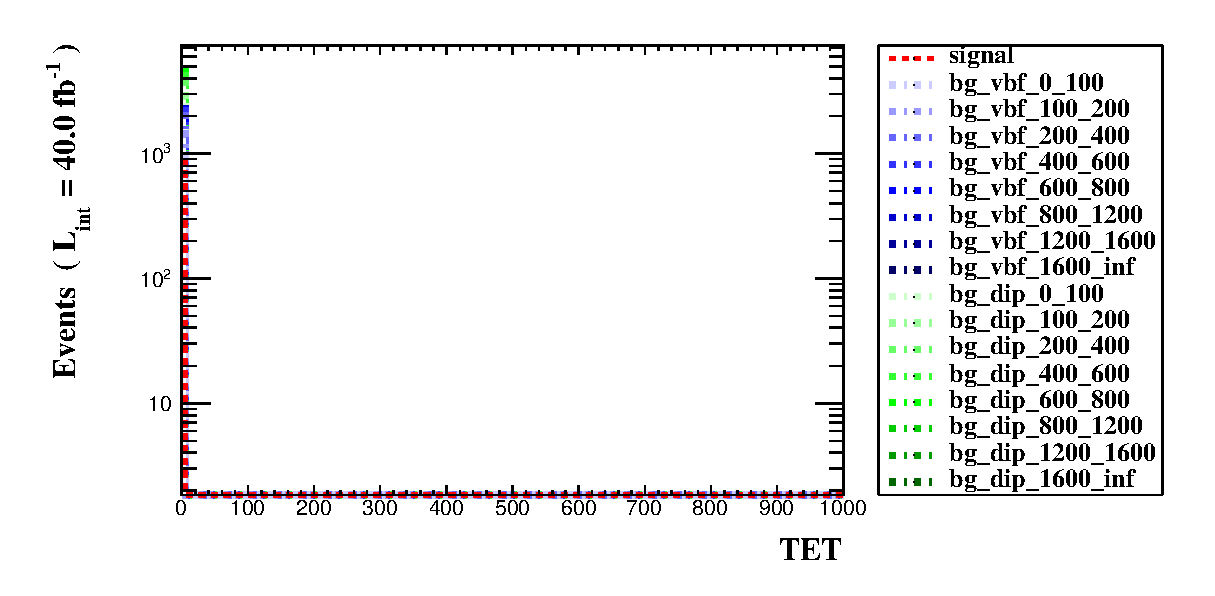
\includegraphics[scale=0.45]{selection_14.eps}\\
\caption{   }
  \end{center}
\end{figure}
      \newpage
\subsection{ Histogram 16}

\textbf{* Plot: TET}\\
   \begin{table}[H]
  \begin{center}
    \begin{tabular}{|m{23.0mm}|m{23.0mm}|m{18.0mm}|m{19.0mm}|m{19.0mm}|m{19.0mm}|m{19.0mm}|}
      \hline
      {\cellcolor{yellow}         Dataset}& {\cellcolor{yellow}         Integral}& {\cellcolor{yellow}         Entries per event}& {\cellcolor{yellow}         Mean}& {\cellcolor{yellow}         RMS}& {\cellcolor{yellow}         \% underflow}& {\cellcolor{yellow}         \% overflow}\\
      \hline
      {\cellcolor{white}         signal}& {\cellcolor{white}         853}& {\cellcolor{white}         1.0}& {\cellcolor{white}         1760.77}& {\cellcolor{white}         810.5}& {\cellcolor{red}         0.0}& {\cellcolor{red}         83.4}\\
      \hline
      {\cellcolor{white}         bg\_vbf\_0\_100}& {\cellcolor{white}         102}& {\cellcolor{white}         1.0}& {\cellcolor{white}         137.744}& {\cellcolor{white}         35.69}& {\cellcolor{green}         0.0}& {\cellcolor{green}         0.0}\\
      \hline
      {\cellcolor{white}         bg\_vbf\_100\_200}& {\cellcolor{white}         477}& {\cellcolor{white}         1.0}& {\cellcolor{white}         223.583}& {\cellcolor{white}         59.29}& {\cellcolor{green}         0.0}& {\cellcolor{green}         0.01051}\\
      \hline
      {\cellcolor{white}         bg\_vbf\_200\_400}& {\cellcolor{white}         573}& {\cellcolor{white}         1.0}& {\cellcolor{white}         387.623}& {\cellcolor{white}         105.1}& {\cellcolor{green}         0.0}& {\cellcolor{green}         0.08151}\\
      \hline
      {\cellcolor{white}         bg\_vbf\_400\_600}& {\cellcolor{white}         174}& {\cellcolor{white}         1.0}& {\cellcolor{white}         628.672}& {\cellcolor{white}         140.2}& {\cellcolor{green}         0.0}& {\cellcolor{green}         2.28}\\
      \hline
      {\cellcolor{white}         bg\_vbf\_600\_800}& {\cellcolor{white}         55.7}& {\cellcolor{white}         1.0}& {\cellcolor{white}         855.907}& {\cellcolor{white}         177.2}& {\cellcolor{red}         0.0}& {\cellcolor{red}         16.73}\\
      \hline
      {\cellcolor{white}         bg\_vbf\_800\_1200}& {\cellcolor{white}         20.2}& {\cellcolor{white}         1.0}& {\cellcolor{white}         1143.56}& {\cellcolor{white}         250.2}& {\cellcolor{red}         0.0}& {\cellcolor{red}         66.96}\\
      \hline
      {\cellcolor{white}         bg\_vbf\_1200\_1600}& {\cellcolor{white}         2.25}& {\cellcolor{white}         1.0}& {\cellcolor{white}         1588.58}& {\cellcolor{white}         315.6}& {\cellcolor{red}         0.0}& {\cellcolor{red}         100.0}\\
      \hline
      {\cellcolor{white}         bg\_vbf\_1600\_inf}& {\cellcolor{white}         0.403}& {\cellcolor{white}         1.0}& {\cellcolor{white}         2087.04}& {\cellcolor{white}         419.9}& {\cellcolor{red}         0.0}& {\cellcolor{red}         100.0}\\
      \hline
      {\cellcolor{white}         bg\_dip\_0\_100}& {\cellcolor{white}         117}& {\cellcolor{white}         1.0}& {\cellcolor{white}         142.783}& {\cellcolor{white}         39.01}& {\cellcolor{green}         0.0}& {\cellcolor{green}         0.0}\\
      \hline
      {\cellcolor{white}         bg\_dip\_100\_200}& {\cellcolor{white}         496}& {\cellcolor{white}         1.0}& {\cellcolor{white}         228.006}& {\cellcolor{white}         64.22}& {\cellcolor{green}         0.0}& {\cellcolor{green}         0.0}\\
      \hline
      {\cellcolor{white}         bg\_dip\_200\_400}& {\cellcolor{white}         814}& {\cellcolor{white}         1.0}& {\cellcolor{white}         393.387}& {\cellcolor{white}         108.5}& {\cellcolor{green}         0.0}& {\cellcolor{green}         0.05657}\\
      \hline
      {\cellcolor{white}         bg\_dip\_400\_600}& {\cellcolor{white}         531}& {\cellcolor{white}         1.0}& {\cellcolor{white}         608.326}& {\cellcolor{white}         127.5}& {\cellcolor{green}         0.0}& {\cellcolor{green}         1.844}\\
      \hline
      {\cellcolor{white}         bg\_dip\_600\_800}& {\cellcolor{white}         263}& {\cellcolor{white}         1.0}& {\cellcolor{white}         810.693}& {\cellcolor{white}         145.6}& {\cellcolor{orange}         0.0}& {\cellcolor{orange}         8.579}\\
      \hline
      {\cellcolor{white}         bg\_dip\_800\_1200}& {\cellcolor{white}         96.6}& {\cellcolor{white}         1.0}& {\cellcolor{white}         1089.47}& {\cellcolor{white}         214.1}& {\cellcolor{red}         0.0}& {\cellcolor{red}         59.21}\\
      \hline
      {\cellcolor{white}         bg\_dip\_1200\_1600}& {\cellcolor{white}         10.8}& {\cellcolor{white}         1.0}& {\cellcolor{white}         1518.09}& {\cellcolor{white}         264.2}& {\cellcolor{red}         0.0}& {\cellcolor{red}         100.0}\\
      \hline
      {\cellcolor{white}         bg\_dip\_1600\_inf}& {\cellcolor{white}         2.03}& {\cellcolor{white}         1.0}& {\cellcolor{white}         2009.95}& {\cellcolor{white}         344.4}& {\cellcolor{red}         0.0}& {\cellcolor{red}         100.0}\\
\hline
    \end{tabular}
  \end{center}
\end{table}

\begin{figure}[H]
  \begin{center}
    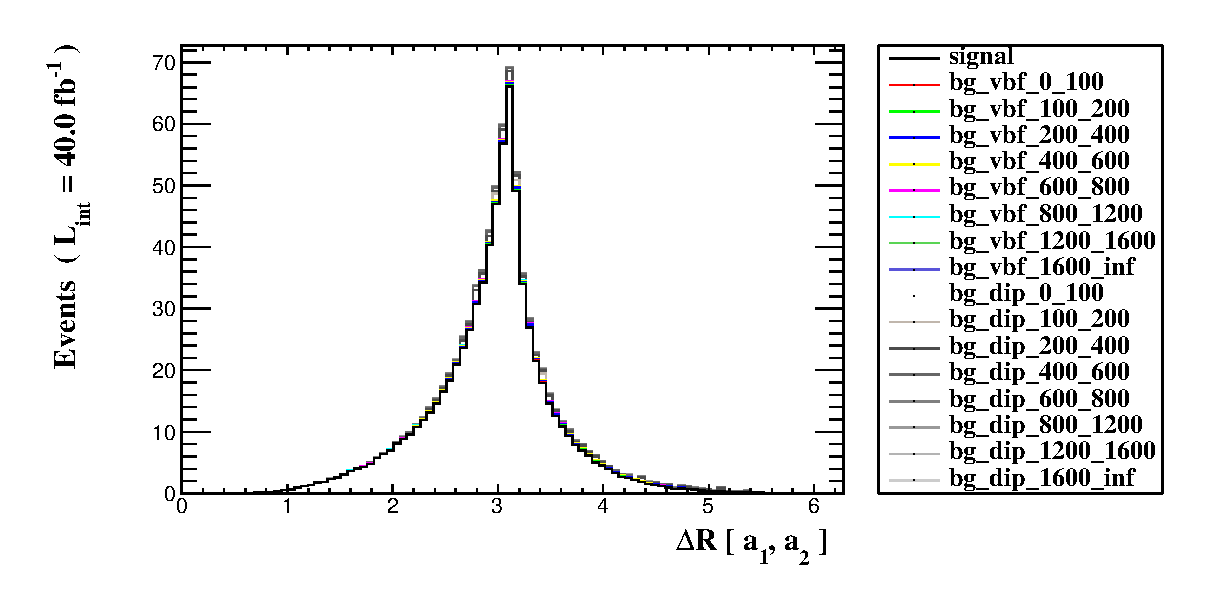
\includegraphics[scale=0.45]{selection_15.eps}\\
\caption{   }
  \end{center}
\end{figure}
      % -----------------------------------------------------------------------------
%                                SECTION Summary                                
% -----------------------------------------------------------------------------
\newpage
\section{ Summary}

\subsection{Cut-flow charts}

\begin{itemize}
  \item How to compare signal (S) and background (B): \textcolor{blue}{S/\-sqrt(S+B)} .
   \item Object definition selections are indicated in cyan.  \item Reject and select are indicated by 'REJ' and 'SEL' respectively
\end{itemize}
\begin{table}[H]
  \begin{center}
    \begin{tabular}{|m{36.0mm}|m{36.0mm}|m{36.0mm}|m{33.0mm}|}
      \hline
      {\cellcolor{yellow}        Cuts}& {\cellcolor{yellow}         Signal (S)}& {\cellcolor{yellow}         Background (B)}& {\cellcolor{yellow}         S vs B}\\
      \hline
      {\cellcolor{white}         Initial (no cut)}& {\cellcolor{white}         4094.08 +/\-- 1.13}& {\cellcolor{white}         4113516 +/\-- 4877}& {\cellcolor{white}         2.01760 +/\-- 0.00132}\\
      \hline
      {\cellcolor{white} SEL: sdETA ( jets[1] jets[2] ) > 2.6 and M ( jets[}& {\cellcolor{white}         853.4 +/\-- 26.0}& {\cellcolor{white}         3739.6 +/\-- 59.9}& {\cellcolor{white}         12.592 +/\-- 0.357}\\
\hline
    \end{tabular}
  \end{center}
\end{table}

\end{document}
